\documentclass[11pt,a4paper]{article}
\usepackage[T1]{fontenc}
\usepackage[utf8]{inputenc}
\usepackage{newtxtext,newtxmath}

\setcounter{tocdepth}{1}
\usepackage[a4paper,margin=35mm]{geometry}
\linespread{0.90}
\setlength{\parindent}{0pt}
\setlength{\parskip}{6pt}
\usepackage{float}
\usepackage{cmap}
\usepackage{amsfonts}
\let\openbox\relax
\usepackage{amsthm}
\usepackage{amsmath}
\usepackage{mathtools}
\allowdisplaybreaks
\usepackage{bm}
\usepackage{graphicx}
\usepackage{tikz}
\usepackage{pgfplots}
\pgfplotsset{compat=1.18}

\hyphenation{superselection}
\usepackage{microtype}
\usepackage[numbers,sort&compress]{natbib}
\usepackage{xcolor}
\usepackage{booktabs}
\usepackage{enumitem}
\usepackage{array}
\usepackage{tabularx}
\usepackage{setspace}
\usepackage[explicit]{titlesec}
\usepackage[labelfont=bf]{caption}
\DeclareCaptionFont{captionthirtysmaller}{\fontsize{7.7}{9.2}\selectfont}
\captionsetup[figure]{font=captionthirtysmaller}
\captionsetup[table]{font=captionthirtysmaller}
\usepackage{mdframed}
\usepackage{needspace}
\usepackage{tocloft}
\usepackage{placeins}
\newcolumntype{Y}{>{\raggedright\arraybackslash}X}
\setlength{\tabcolsep}{4.5pt}
\renewcommand{\arraystretch}{1.1}
\renewcommand{\qedsymbol}{}
\AtBeginEnvironment{tabular}{\small}
\AtBeginEnvironment{tabularx}{\small}

\numberwithin{equation}{section}
% Automatic equation numbering enabled for displayed equations
\mathtoolsset{showonlyrefs=false}
\DeclarePairedDelimiter{\abs}{\lvert}{\rvert}
\DeclarePairedDelimiter{\norm}{\lVert}{\rVert}
\DeclareMathOperator{\Tr}{Tr}
\DeclareMathOperator{\diag}{diag}
\DeclareMathOperator{\rank}{rank}
\newcommand{\dd}{\mathrm{d}}
\newcommand{\ii}{\mathrm{i}}

\setlist{nosep,leftmargin=1.25em}

\titleformat{\section}
{\normalfont\normalsize\bfseries\raggedright}
{\thesection}{0.75em}{\begin{minipage}[t]{0.9\textwidth}#1\end{minipage}}
[\vspace{0.12em}\titlerule]

\newcommand{\subaccent}{\vspace{0.01em}\noindent\rule{7ex}{0.2pt}}
\titleformat{\subsection}
{\normalfont\normalsize\bfseries}{\thesubsection}{0.5em}{#1}
[\subaccent]
\titlespacing*{\subsection}{0pt}{2.2ex plus 0.6ex}{1.5ex}

\titleformat{\subsubsection}
{\normalfont\normalsize\bfseries}{\thesubsubsection}{0.5em}{#1}
\titlespacing*{\subsubsection}{0pt}{1.6ex plus 0.4ex}{0.6ex}

\usepackage[
  pdfusetitle,
  hidelinks,
  bookmarksopen=true,
  bookmarksnumbered=true
]{hyperref}

\newtheoremstyle{thmcompact}
{0.5ex}{0.5ex}
{\itshape}
{0pt}
{\bfseries}
{.}
{0.6em}
{\thmname{#1}\ \thmnumber{#2}\ \thmnote{(\textit{#3})}}

\theoremstyle{thmcompact}
\newtheorem{theorem}{Theorem}[section]
\newtheorem{proposition}[theorem]{Proposition}
\newtheorem{lemma}[theorem]{Lemma}
\newtheorem{corollary}[theorem]{Corollary}
\newtheorem{definition}[theorem]{Definition}

\theoremstyle{remark}
\newtheorem*{remarkplain}{Remark}

\mdfdefinestyle{thmframe}{%
	leftline=true, rightline=false, topline=false, bottomline=false,
	linewidth=0.8pt, linecolor=black,
	innerleftmargin=16pt, innerrightmargin=8pt,
	innertopmargin=6pt, innerbottommargin=6pt,
	skipabove=6pt, skipbelow=6pt,
	nobreak=true
}
\surroundwithmdframed[style=thmframe]{theorem}
\surroundwithmdframed[style=thmframe]{proposition}
\surroundwithmdframed[style=thmframe]{lemma}
\surroundwithmdframed[style=thmframe]{corollary}
\surroundwithmdframed[style=thmframe]{definition}

\newmdenv[
linewidth=0.6pt,
topline=false,
bottomline=false,
rightline=false,
skipabove=\baselineskip,
skipbelow=\baselineskip,
backgroundcolor=gray!3,
leftmargin=0pt,
innerleftmargin=8pt,
innerrightmargin=6pt,
frametitleaboveskip=0.4em,
frametitlebelowskip=0.2em,
frametitlefont=\bfseries\small,
]{remarkbox}
\usepackage{titling}
\newenvironment{remark}[1][]%
{\begin{remarkbox}\begin{remarkplain}[#1]\normalfont}
		{\end{remarkplain}\end{remarkbox}}

\renewcommand{\contentsname}{Contents}

\titleformat{name=\section,numberless}
{\normalfont\normalsize\bfseries\raggedright}
{}{0em}{\begin{minipage}[t]{0.9\textwidth}#1\end{minipage}}
[\vspace{0.12em}\titlerule]
\makeatletter
\renewcommand{\l@section}[2]{\@dottedtocline{1}{0em}{2.3em}{\raggedright #1}{#2}}
\renewcommand{\l@subsection}[2]{\@dottedtocline{2}{1.8em}{3.2em}{\raggedright #1}{#2}}
\makeatother

\emergencystretch=3em
\hfuzz=1pt
\tolerance=1800
\hbadness=2500

\newcommand{\thmneed}{\Needspace{6\baselineskip}}
\AtBeginEnvironment{theorem}{\thmneed}
\AtBeginEnvironment{proposition}{\thmneed}
\AtBeginEnvironment{lemma}{\thmneed}
\AtBeginEnvironment{corollary}{\thmneed}

\AtBeginEnvironment{thebibliography}{\small}

\title{\textbf{Finite Observation}\\[0.2em]
\large A Spectral Theory of Nonequilibrium Visibility}
\author{J.\,R.~Dunkley}
\date{18th March 2026}

\hypersetup{
  pdftitle={Finite Observation: A Spectral Theory of Nonequilibrium Visibility},
  pdfauthor={J. R. Dunkley},
  pdfsubject={Finite-dimensional nonequilibrium visibility, Donsker--Varadhan Hessian, weighted spectral compression},
  pdfkeywords={nonequilibrium steady states, Donsker--Varadhan, Fisher geometry, Ky Fan envelope, visibility, detectability, Markov chains, Gaussian fluctuations},
  pdfproducer={pdfLaTeX}
}

\begin{document}

\maketitle

\begin{abstract}
We study finite observation in irreducible finite-state continuous-time Markov nonequilibrium steady states through the local Donsker–Varadhan Hessian at the steady-state minimiser. In reduced Fisher coordinates, the nonequilibrium correction factors through a weighted signal operator and the detailed-balance backbone. For fixed-rank orthogonal observation in this reduced Euclidean Fisher geometry, the visible correction is controlled by a Ky Fan envelope, together with an associated retention hierarchy, hidden tail, and weighted stable rank. This hierarchy determines the spectral profile of the visible nonequilibrium correction and, equivalently, the corresponding singular-energy profile of the weighted signal operator, and therefore its nonzero singular-value magnitudes. We also identify the optimal orthogonal observer at fixed rank and show that a Haar-random rank-constrained observer retains, on average, exactly the corresponding dimensional fraction of the available signal. A separate statistical question arises after comparison with the observed detailed-balance backbone: in the compressed-Hessian Gaussian model, distinguishability is governed by a positive shadow operator whose spectrum can differ from the raw visibility spectrum except in special commuting or isotropic-backbone regimes. The same weighted geometry extends to abstract finite-dimensional metric settings, and hence to the linearised BKM-symmetrised operator setting.
\end{abstract}

\newpage

\tableofcontents

\newpage

\section{Introduction}
\label{sec:introduction}

\subsection{The finite observation problem}

A nonequilibrium system may carry irreversibility across many microscopic directions while only a small observable sector is accessible. Hidden transitions, finite time resolution, finite spatial resolution, detector noise, and coarse graining all lead to the same structural question: what can a finite observer actually see of the nonequilibrium fluctuation structure?

In finite-dimensional Markov nonequilibrium steady states, the natural empirical-measure fluctuation object is the local Hessian of the Donsker--Varadhan rate function at its minimiser \(\pi\) \cite{DonskerVaradhan1975a,DonskerVaradhan1975b,Touchette2009,LebowitzSpohn1999}. A finite observer does not see the full Hessian. The observer only sees its compression to a rank-limited sector. The finite observation problem is therefore precise: given an irreducible nonequilibrium generator and an observable subspace of dimension \(d\), how much of the nonequilibrium correction survives projection, and how does that visible share depend on the geometry of the system and the geometry of the observer? The detailed-balance geometry is the reference geometry adopted here for measuring this local Gaussian nonequilibrium correction.

We show that, in the finite-dimensional Markov Gaussian regime treated here, this question reduces to a spectral compression problem in reduced Fisher coordinates. The visible share is governed by a weighted singular-value hierarchy. The hidden share is its spectral tail. The effective complexity of visibility is controlled by weighted stable rank.

\subsection{Motivation}

Recent work across stochastic thermodynamics, coarse graining, and quantum nonequilibrium theory has made the finite observation problem sharper and more urgent. The literature contains lower bounds on entropy production under partial observation, hidden data, coarse temporal sampling, unresolved transitions, faulty observation maps, and coarse graining \cite{BaiesiNishiyamaFalasco2023,FritzErtelSeifert2024,Harunari2024,vanderMeerSaito2025,ErtelSeifert2025,Ehrich2021,DeguntherVanDerMeerSeifert2024,Esposito2012}. Closely related work studies estimator quality for dissipation under lumping, milestoning, hidden cycles, current fluctuations, and finite statistics, and proposes random or optimised coarse-graining strategies for irreversibility detection \cite{BlomSongVougaGodecMakarov2025,BaoOhgaIto2025,GingrichRotskoffHorowitz2017,YuLeightonLynn2025,TezaStellaGrandPre2025,TezaStella2020}.

Restricted-information and coarse-grained quantum thermodynamics make the same point from another direction: observation changes the effective thermodynamic description \cite{RubinoBruknerManzano2025,PernambucoCeleri2026,LacerdaBettmannGoold2025,BettmannGoold2025,Wirth2025}. At a broader level, the thermodynamic uncertainty-relation programme has clarified how much of the field is organised around scalar fluctuation bounds rather than observer-resolved spectral structure \cite{BaratoSeifert2015,HorowitzGingrich2020}, and very recent counterexamples show that even two widely used model-free partial-observation bounds, the waiting-time and TUR bounds, admit no universal ordering on the same observed link \cite{Gu2026}.

What is missing from this landscape, as far as we are aware, is a finite-dimensional law for the visible share of the nonequilibrium correction itself in the Markov Gaussian setting treated here. The current literature is rich in estimators, bounds, and coarse-grained descriptions. The contribution of the present paper is to identify, for orthogonal rank-constrained observers in reduced Euclidean Fisher coordinates, the envelope of the projected Donsker--Varadhan correction, the associated observer-design law at fixed rank, the shadow criterion for observed Gaussian indistinguishability in the compressed-Hessian model, and the corresponding spectral readout of the hidden correction.

\subsection{Main claim and conceptual picture}

The central claim is that finite observation in the Donsker--Varadhan Gaussian regime has a finite-dimensional spectral normal form. In reduced Euclidean Fisher coordinates, the nonequilibrium correction factors through the reduced skew channel and the detailed-balance backbone via the weighted signal map \(A_{DV}\). Finite observation therefore becomes a rank-constrained orthogonal compression problem for that map.

This leads to two distinct spectral questions. The first is raw visibility: how much nonequilibrium signal survives projection, how much is hidden in the spectral tail, and which observer of rank \(d\) is best aligned with the signal front. That question is governed by the singular spectrum of \(A_{DV}\) and the associated Ky Fan envelope hierarchy.

The second is detectability relative to the detailed-balance backbone: once the observed correction is compared to the observed backbone in its natural metric, a second positive operator appears, and its spectrum governs Gaussian distinguishability. These two spectra coincide only in special commuting or isotropic-backbone regimes. The raw and detectability spectra therefore read the same nonequilibrium deviation in two different equilibrium coordinate systems: the ambient detailed-balance backbone, and the backbone induced on the observed sector after projection. Raw nonequilibrium signal and statistically detectable nonequilibrium signal therefore need not live in the same observer directions. The theory therefore distinguishes directions that are structurally invisible under the observation map from directions that remain visible in principle but are weak or poorly aligned in the observable geometry.

Within the orthogonal-observer model used here, the paper gives a finite-dimensional theory of visibility, observer design, detectability, and spectral readout. The bridge theorem identifies the structure of the correction, the envelope gives the visible law, the shadow gives the distinguishability law, and the full hierarchy recovers the singular-energy profile of the correction, equivalently the nonzero singular-value magnitudes of \(A_{DV}\).

\subsection{Main results}

\textbf{The first result is the bridge theorem.} We prove that the Donsker--Varadhan correction is quadratic in the reduced skew channel. This is the representation step that turns the fluctuation problem into a weighted operator problem.

\textbf{The second result is the finite-observation law.} For every orthogonal rank-constrained observer, the visible nonequilibrium content is given by a Ky Fan envelope of the weighted signal map. The retention hierarchy, hidden tail, and weighted stable rank follow from this representation.

\textbf{The third result is the observer-design law.} Visible signal is an alignment score against the left singular modes of the weighted signal map. This yields the optimal orthogonal observer, its gap-controlled uniqueness criterion, the worst observer, and the Haar-random rank-\(d\) baseline in expectation.

\textbf{The fourth result is the two-spectrum theorem.} The observed Gaussian law in the compressed-Hessian model is governed by a positive shadow operator, and backbone whitening yields a second spectral hierarchy for detectability relative to the detailed-balance backbone. In general this detectability spectrum is distinct from the raw visibility spectrum.

\textbf{The fifth result is spectral completeness of the envelope hierarchy for magnitudes.} The full envelope hierarchy recovers the ordered singular-energy profile \(\tfrac14 s_k(A_{DV})^2\), equivalently the eigenvalue profile of \(\Delta_{DV}\), and hence the nonzero singular-value magnitudes of \(A_{DV}\).

\textbf{The sixth result is a transfer theorem.} The weighted visibility, envelope, alignment, and spectral-readout structure transfer to abstract finite-dimensional metric settings and hence to linearised BKM operator geometry.

\subsection{Contribution}

The paper gives a finite-dimensional structural solution of the orthogonal-observer problem of finite observation in the Markov Gaussian regime treated here. Its contribution is to identify the operator geometry that organises what finite observers can still see within that model.

More specifically, it proves a bridge from the skew sector to the fluctuation correction, a rank-constrained envelope law, an observer-design law with a Haar baseline, a Gaussian shadow criterion, a second spectrum for detectability distinct from raw visibility, and an envelope hierarchy that determines the singular-energy profile of the correction and hence the singular-value magnitudes of \(A_{DV}\).

\subsection{Roadmap}

Section~\ref{sec:setting-observable-normal-forms} fixes the finite-dimensional Markov setting, the Fisher normal form, the notion of a finite observer, and the observable normal-form language. Section~\ref{sec:exact-dv-bridge} proves the bridge theorem and identifies the nonequilibrium correction as a positive correction operator together with its weighted signal factorisation. Section~\ref{sec:observable-envelope} derives the finite-observation law: the Ky Fan envelope, retention hierarchy, hidden tail, stable-rank obstruction, and the direct-sum allocation reading of the envelope.

Section~\ref{sec:alignment-optimal-observers} develops the observer-design layer through the alignment theorem, optimal and worst observers, and the Haar-random baseline. Section~\ref{sec:shadow-operator-gaussian-distinguishability} proves the shadow and detectability theory, making explicit the split between raw visibility and backbone-normalised distinguishability, and includes a fixed-channel Gaussian noisy-observation extension. Section~\ref{sec:spectroscopy-hidden-structure} proves spectral completeness of the envelope hierarchy for singular-value magnitudes and develops the induced observability order between systems.

\section{Setting and observable normal forms}
\label{sec:setting-observable-normal-forms}

\subsection{Finite-dimensional Markov nonequilibrium steady states}

Let \(\mathsf X=\{1,\dots,n\}\) be a finite state space, and let \(Q\) be the generator of an irreducible continuous-time Markov chain on \(\mathsf X\). Thus \(Q_{ij}\ge 0\) for \(i\neq j\), \(\sum_j Q_{ij}=0\) for each \(i\), and irreducibility guarantees a unique stationary law
\begin{equation}
\pi=(\pi_1,\dots,\pi_n),\qquad \pi_i>0,\qquad \sum_i \pi_i=1,
\end{equation}
satisfying \(\pi Q=0\). We are interested in the nonequilibrium steady-state case, meaning that \(Q\) need not satisfy detailed balance with respect to \(\pi\).

Throughout the paper we work at the level of stationary empirical-measure fluctuations. The fluctuation object in this setting is the local Hessian of the Donsker--Varadhan rate function at its minimiser \(\pi\), viewed in the Fisher geometry associated with the stationary law. This Fisher viewpoint is not merely convenient notation: in nonequilibrium stochastic thermodynamics it has a direct geometric and physical interpretation, and in the reversible Markov setting it sits on a well-developed information-geometric background \cite{Ito2018,WolferWatanabe2021}. The detailed-balance geometry provides the reference unit system in which the Gaussian nonequilibrium correction is measured. The entire finite-observation theory developed below takes place in the tangent space at \(\pi\), after passing to the Euclideanised Fisher coordinates adapted to that geometry.

Let
\begin{equation}
D_\pi:=\mathrm{diag}(\pi_1,\dots,\pi_n),
\qquad
e_\pi:=\bigl(\sqrt{\pi_1},\dots,\sqrt{\pi_n}\bigr)^T.
\end{equation}
The Euclideanised Fisher tangent space is
\begin{equation}
T_\pi
:=
\{u\in\mathbb R^n:\langle u,e_\pi\rangle=0\}.
\end{equation}
Equivalently, \(T_\pi\) is the codimension-one subspace orthogonal to the stationary direction in Fisher coordinates. We denote by
\begin{equation}
P_\pi:=I-e_\pi e_\pi^T
\end{equation}
the orthogonal projector onto \(T_\pi\).

The Fisher metric in density coordinates becomes the standard Euclidean inner product after this transformation, so from this point onward all orthogonality, projection, adjoints, and singular values in the classical Markov setting are taken with respect to the Euclidean structure on \(T_\pi\), unless stated otherwise.

\subsection{Fisher geometry and the normal form}

Define the Fisher-conjugated generator
\begin{equation}
L_\pi:=D_\pi^{1/2} Q D_\pi^{-1/2}.
\end{equation}
Its restriction to the tangent space carries the full linearised stationary fluctuation geometry. Since \(T_\pi\) is \(L_\pi\)-invariant, we may regard
\begin{equation}
K:=L_\pi|_{T_\pi}
\end{equation}
as an operator on \(T_\pi\).

The central structural decomposition is the Fisher normal form
\begin{equation}
K=G+J,
\end{equation}
where
\begin{equation}
G:=\frac{K+K^T}{2},
\qquad
J:=\frac{K-K^T}{2}.
\end{equation}
Thus \(G\) is self-adjoint and \(J\) is skew-adjoint on \(T_\pi\). In the present work, \(G\) is the dissipative backbone and \(J\) is the skew, antisymmetric sector carrying the nonequilibrium part relative to the detailed-balance backbone. This symmetric\/antisymmetric normal-form viewpoint is consonant with earlier steady-state fluctuation analyses of driven diffusions \cite{MaesNetocnyWynants2008} and with the network-cycle description of nonequilibrium steady states originating in Schnakenberg theory \cite{Schnakenberg1976}. The detailed-balance reference object is obtained by setting \(J=0\) while keeping the same stationary law and dissipative geometry.

The nonequilibrium correction to the Donsker-Varadhan Hessian will be shown in Section~
ef{sec:exact-dv-bridge} to be carried entirely by the skew sector after the reduced-coordinate analysis, while the observed detailed-balance backbone is governed by the projected dissipative sector.

To work concretely, choose an orthonormal matrix
\begin{equation}
C\in\mathbb R^{n\times (n-1)}
\end{equation}
whose columns form an orthonormal basis of \(T_\pi\). Then
\begin{equation}
C^T C=I_{n-1},
\qquad
CC^T=P_\pi.
\end{equation}
Reduced coordinates \(x\in\mathbb R^{n-1}\) are identified with tangent vectors by \(u=Cx\). In these coordinates the Fisher-conjugated generator becomes
\begin{equation}
\widehat K:=C^T L_\pi C,
\end{equation}
with corresponding reduced decomposition
\begin{equation}
\widehat K=\widehat G+\widehat J,
\qquad
\widehat G=\frac{\widehat K+\widehat K^T}{2},
\qquad
\widehat J=\frac{\widehat K-\widehat K^T}{2}.
\end{equation}
All finite-dimensional statements in the main text will be expressed on this reduced Euclidean space. For notational simplicity, we will often suppress the distinction between the operator on \(T_\pi\) and its matrix in reduced coordinates when no ambiguity arises. Where the reduced-coordinate nature matters, hats will be retained. This dissipative-plus-skew normal form already foreshadows the later operator-space transfer, where the same structural split reappears in metric operator geometry.

\subsection{Observable sectors and finite observers}

A finite observer is modelled by a rank-constrained orthogonal projector on the reduced Fisher space. Concretely, let
\begin{equation}
\Pi:\mathbb R^{n-1}\to\mathbb R^{n-1}
\end{equation}
be a Euclidean orthogonal projector of rank \(d\), and let
\begin{equation}
U:=\operatorname{Ran}\Pi.
\end{equation}
The rank \(d\) is the observable dimension. It is the number of independent fluctuation directions actually accessible to the observer.

This choice of projector is the mathematical form of finite observation used here. It covers rank-constrained observable sectors, reduced coordinates, compressions to slow manifolds, and more abstract finite-resolution measurement ideals, provided the observation is represented by orthogonal compression in the underlying Euclideanised geometry. The exact envelope law proved below is for orthogonal rank-\(d\) observers in this sense. More general coarse-graining maps require different machinery, with the fixed-channel Gaussian noisy-observation section giving one controlled extension. Later sections will explain how this structure extends to weighted operator-space settings, where orthogonality is taken with respect to a nontrivial metric.

Given \(\Pi\), the observer does not see the full operator \(K\), the full detailed-balance Hessian, or the full Donsker-Varadhan Hessian. The observer sees only their compressions to \(U\). The finite observation problem is therefore a rank-constrained compression problem on a fluctuation operator whose full structure is initially hidden.

\subsection{Projected observable normal forms}

The projected observable normal form associated with \(\Pi\) is
\begin{equation}
N_\Pi(Q):=(U,g_\Pi,G_\Pi,J_\Pi),
\end{equation}
where \(g_\Pi\) is the Euclidean metric restricted to \(U\), and
\begin{equation}
G_\Pi:=\Pi \widehat G \Pi|_U,
\qquad
J_\Pi:=\Pi \widehat J \Pi|_U.
\end{equation}
This is the observable quadruple inherited by finite observation from the full Markov generator.

Observable equivalence is governed by such projected data once the finer nonequilibrium correction is sufficiently small. The work proves a stronger result. The projected quadruple is the observable backbone of a signal theory in which the nonequilibrium correction is placed in weighted spectral form and its visible share under \(\Pi\) is determined explicitly.

Three levels of observable structure will later reappear:

\begin{enumerate}
\item the purely metric or static level, carried by \(U\) and \(g_\Pi\),
\item the dissipative level, carried by \(G_\Pi\),
\item the full projected normal form, carried by \((g_\Pi,G_\Pi,J_\Pi)\).
\end{enumerate}

The theory developed below refines this hierarchy by inserting one more object: the projected nonequilibrium correction to the Donsker-Varadhan Hessian. That correction is the signal of hidden irreversibility.

\subsection{The Donsker-Varadhan Hessian as the fluctuation object}

Let \(I_{DV}\) denote the Donsker-Varadhan rate function for the empirical measure of the irreducible Markov chain generated by \(Q\). Since \(\pi\) is the unique stationary law, \(\pi\) is the minimiser of \(I_{DV}\), and the Hessian of \(I_{DV}\) at \(\pi\) is positive definite on the reduced tangent space. We denote this Hessian in reduced Euclidean coordinates by
\begin{equation}
H_{DV}.
\end{equation}

The canonical detailed-balance reference is obtained by Fisher symmetrisation. Let
\begin{equation}
L_\pi:=D_\pi^{1/2}QD_\pi^{-1/2},
\qquad
G_{\mathrm{full}}:=\frac12(L_\pi+L_\pi^T),
\qquad
Q_0:=D_\pi^{-1/2}G_{\mathrm{full}}D_\pi^{1/2}.
\end{equation}
Then \(Q_0\) has the same stationary law \(\pi\), satisfies detailed balance with respect to \(\pi\), and has reduced Fisher generator \(\widehat G\). The corresponding detailed-balance Hessian on the reduced Euclidean Fisher space is therefore
\begin{equation}
H_0:=-\frac12\,\widehat G.
\end{equation}
Because the detailed-balance reference is irreducible, \(-\widehat G\) is positive definite on the reduced space, so \(H_0\succ 0\) and is therefore invertible there. Under this sign convention, the positive conductance form is represented by \(-\widehat G\).
The nonequilibrium correction is
\begin{equation}
\Delta_{DV}:=H_{DV}-H_0.
\end{equation}
At this point, \(\Delta_{DV}\) is only a definition. The bridge section then identifies it as a positive correction operator built from the skew sector and the detailed-balance backbone.

The object of interest is not entropy production by itself, nor the full rate function, nor a pathwise current observable. It is the fluctuation-side nonequilibrium correction encoded in \(H_{DV}\). Once that correction is understood, finite observation becomes a problem of spectral retention.

\section{The Donsker-Varadhan bridge}
\label{sec:exact-dv-bridge}

\subsection{Reduced coordinates and the conductance identity}

The bridge from the Donsker-Varadhan variational principle to the spectral theory developed later in the paper passes through a reduced-coordinate quadratic envelope. The full derivation is carried out in Appendix~A. Here we isolate the structural cancellation that drives everything that follows.

Starting from the variational representation of the Donsker-Varadhan rate function, one introduces reduced logarithmic coordinates near stationarity and expands the envelope to second order. This produces a reduced quadratic fluctuation problem governed by two coupled ingredients. One is a current-like reduced operator carrying the skew dependence. The other is a reduced conductance matrix controlling the quadratic envelope itself. A priori, both the dissipative and skew sectors could have entered that conductance matrix.

They do not. The skew sector contributes no quadratic form of its own, so the conductance matrix of the full nonequilibrium envelope depends only on the dissipative backbone. This is the reason the final bridge is purely quadratic in the skew channel, with no mixed dissipative-skew leakage.

Let \(M_Q\) denote the reduced conductance matrix produced by the full nonequilibrium envelope construction, and let \(M_G\) denote the corresponding reduced conductance matrix for the detailed-balance reference problem obtained by suppressing the skew sector. Both objects are defined canonically by the same reduced-coordinate construction; the explicit formulas are recorded in Appendix~A.

\begin{proposition}[Reduced conductance identity]
\label{prop:reduced_conductance_identity}
In the finite-dimensional irreducible Markov setting described above, the reduced conductance matrix of the full Donsker-Varadhan quadratic envelope coincides with that of the detailed-balance reference problem:
\begin{equation}
M_Q=M_G.
\end{equation}
Equivalently, the quadratic conductance controlling the reduced Donsker-Varadhan Hessian depends only on the dissipative sector and is blind to the skew sector.
\end{proposition}

\begin{proof}
Write the Donsker--Varadhan variational formula as \cite{DonskerVaradhan1975a,DonskerVaradhan1975b,Touchette2009}
\begin{equation}
I_{DV}(\mu)=\sup_h\Bigl(-\sum_{i,j}\mu_i q_{ij}(e^{h_j-h_i}-1)\Bigr).
\end{equation}
Choose reduced Fisher coordinates \(x\in\mathbb R^{n-1}\) and reduced logarithmic coordinates \(y\in\mathbb R^{n-1}\) by
\begin{equation}
\mu(x)=\pi+D_\pi^{1/2}Cx+O(|x|^2),
\qquad
h(y)=D_\pi^{-1/2}Cy.
\end{equation}
Using the second-order reduced-coordinate expansion derived in Appendix~\ref{app:reduced_coordinate_identities} gives the reduced quadratic envelope
\begin{equation}
\mathcal L(x,y)=y^T\widehat G y-x^T\widehat K y+O(|(x,y)|^3),
\end{equation}
where \(\widehat K=C^TD_\pi^{1/2}QD_\pi^{-1/2}C=\widehat G+\widehat J\). The key point is that the pure quadratic term in \(y\) is
\begin{equation}
y^T\widehat K y=y^T\widehat G y,
\end{equation}
because \(y^T\widehat J y=0\) for every skew-symmetric matrix \(\widehat J\). Hence the conductance block is determined entirely by \(\widehat G\), and the nonequilibrium reduced conductance coincides with the detailed-balance one. Equivalently,
\begin{equation}
M_Q=M_G=-\widehat G.
\end{equation}
The skew sector survives only in the current block \(-x^T\widehat K y\).
\end{proof}

Proposition~\ref{prop:reduced_conductance_identity} records the key asymmetry used in the bridge argument. The skew sector drives the nonequilibrium correction, but the quadratic conductance beneath the reduced envelope is controlled by the dissipative geometry alone. This is why the later factorisation of the correction is so rigid. The skew sector enters through a weighted signal map, but the weight itself is fixed by the detailed-balance backbone. The first antisymmetry input here is the identity \(y^T\widehat J y=0\), but the bridge theorem uses it inside the Legendre contraction, where the supremum over \(y\) removes the mixed dissipative-skew contribution at Hessian order. This cancellation is a level-2 empirical-measure statement, and should not be read as a statement about the unreduced level-2.5 fluctuation Hessian.

The rest of Section~\ref{sec:exact-dv-bridge} exploits this asymmetry. The next subsection converts the reduced envelope into a quadratic representation of the nonequilibrium correction, which in turn becomes the signal operator governing finite observation.

\begin{remark}[Dirac-analogous factorisation of the DV Hessian]
\label{rem:dirac-factorisation}
The bridge identity also admits a canonical first-order factorisation, using the
principal positive square root of \(H_0\). Define
\begin{equation}
D := H_0^{1/2} + \tfrac{1}{2}H_0^{-1/2}\widehat{J}^T.
\label{eq:dirac-operator}
\end{equation}
Since \(\widehat{J}\) is skew-symmetric, one has
\begin{equation}
D^T
=
H_0^{1/2} + \tfrac{1}{2}\widehat{J}H_0^{-1/2},
\end{equation}
and therefore
\begin{equation}
D^T D
=
H_0 + \tfrac{1}{4}\widehat{J}H_0^{-1}\widehat{J}^T
=
H_{DV}.
\label{eq:dirac-factorisation}
\end{equation}
Thus \(H_{DV}=D^T D\) exactly. Since \(H_{DV}\succ 0\) on the reduced space,
\(\ker D=\{0\}\), so \(D\) is invertible. The operator \(D\) packages the
detailed-balance backbone and the reduced skew channel into a single
first-order object whose adjoint square recovers the full nonequilibrium
fluctuation Hessian.
\end{remark}

\subsection{Quadraticity of the nonequilibrium correction}

We now progress to the central bridge theorem. Proposition~\ref{prop:reduced_conductance_identity} implies that the reduced Donsker-Varadhan quadratic envelope is built on the detailed-balance conductance matrix alone. The skew sector therefore enters only through the reduced current channel. This yields a quadratic representation of the nonequilibrium correction.

To state the result cleanly, recall from Section~\ref{sec:setting-observable-normal-forms} that the canonical detailed-balance reference is the Fisher-symmetrised one, with reduced Hessian
\begin{equation}
H_0=-\frac12\,\widehat G.
\end{equation}
Let \(\widehat J\) denote the canonical reduced skew channel produced by the reduced-coordinate envelope construction. The next theorem is the finite-dimensional bridge identity that identifies the fluctuation correction as a positive correction operator with an explicit weighted signal factorisation.

\begin{theorem}[Quadraticity of the DV correction]
\label{thm:exact_quadraticity}
In the finite-dimensional irreducible Markov setting of Section~\ref{sec:setting-observable-normal-forms}, the Donsker-Varadhan Hessian decomposes as

\[
\begingroup
\setlength{\fboxsep}{8pt}%
\setlength{\fboxrule}{1.15pt}%
\boxed{\scalebox{1.08}{$\displaystyle H_{DV}=H_0+\Delta_{DV}$}}%
\endgroup
\]

\begin{center}
where the nonequilibrium correction is
\end{center}
\[
\begingroup
\setlength{\fboxsep}{8pt}%
\setlength{\fboxrule}{1.15pt}%
\boxed{\scalebox{1.08}{$\displaystyle \Delta_{DV}=\frac14\,\widehat J\,H_0^{-1}\widehat J^{T}$}}%
\endgroup
\]

Equivalently, \(\Delta_{DV}\) is positive semidefinite and is quadratic in the reduced skew channel with no mixed dissipative-skew term.
\end{theorem}


\begin{proof}
By Proposition~\ref{prop:reduced_conductance_identity} and the reduced-coordinate expansion recalled above, the second-order reduced envelope has the form
\begin{equation}
\mathcal L(x,y)=y^T\widehat G y-x^T\widehat K y+O(|(x,y)|^3),
\qquad
\widehat K=\widehat G+\widehat J.
\end{equation}
Set
\begin{equation}
S:=-\widehat G.
\end{equation}
Then \(S\) is positive definite on the reduced space and
\begin{equation}
\mathcal L(x,y)
=
-y^TSy+x^T(S-\widehat J)y+O(|(x,y)|^3)
=
-y^TSy+y^T(S+\widehat J)x+O(|(x,y)|^3),
\end{equation}
using \(\widehat J^T=-\widehat J\). Completing the square in \(y\) gives
\begin{equation}
\mathcal L(x,y)
=
-\Bigl(y-\frac12S^{-1}(S+\widehat J)x\Bigr)^TS\Bigl(y-\frac12S^{-1}(S+\widehat J)x\Bigr)
+\frac14 x^T(S+\widehat J)^TS^{-1}(S+\widehat J)x
+O(|(x,y)|^3).
\end{equation}
Taking the supremum over \(y\), exactly as in the reduced variational contraction derived in Appendix~\ref{app:reduced_coordinate_identities}, yields
\begin{equation}
I_{DV}(\mu(x))
=
\frac14 x^T(S+\widehat J)^TS^{-1}(S+\widehat J)x+O(|x|^3).
\end{equation}
Since \(\widehat J^T=-\widehat J\),
\begin{equation}
(S+\widehat J)^TS^{-1}(S+\widehat J)
=
(S-\widehat J)S^{-1}(S+\widehat J)
=
S-\widehat J S^{-1}\widehat J
=
S+\widehat J S^{-1}\widehat J^T.
\end{equation}
Therefore
\begin{equation}
I_{DV}(\mu(x))
=
\frac14 x^T\bigl(S+\widehat J S^{-1}\widehat J^T\bigr)x+O(|x|^3).
\end{equation}
By definition of the reduced Hessian,
\begin{equation}
I_{DV}(\mu(x))=\frac12 x^T H_{DV}x+O(|x|^3),
\end{equation}
so
\begin{equation}
H_{DV}=\frac12 S+\frac12\widehat J S^{-1}\widehat J^T.
\end{equation}
For the detailed-balance reference \(\widehat J=0\), the same reduced envelope gives
\begin{equation}
H_0=\frac12S=-\frac12\widehat G.
\end{equation}
Hence \(H_0^{-1}=2S^{-1}\), and substitution gives
\begin{equation}
H_{DV}=H_0+\frac14\,\widehat J H_0^{-1}\widehat J^T.
\end{equation}
Equivalently,
\begin{equation}
\Delta_{DV}=H_{DV}-H_0=\frac14\,\widehat J H_0^{-1}\widehat J^T.
\end{equation}
The Gram form
\begin{equation}
\Delta_{DV}=\frac14\bigl(\widehat J H_0^{-1/2}\bigr)\bigl(\widehat J H_0^{-1/2}\bigr)^T
\end{equation}
implies positive semidefiniteness.
\end{proof}

\begin{remark}[Orthogonal invariance of the quadratic correction]
The identity of Theorem~\ref{thm:exact_quadraticity} is invariant under orthogonal changes of reduced Euclidean Fisher coordinates. In particular, the spectrum of \(\Delta_{DV}\), and therefore every envelope, retention, and spectral-readout quantity derived from it, is coordinate-independent within the reduced Euclidean Fisher coordinates fixed by the paper.
\end{remark}

Theorem~\ref{thm:exact_quadraticity} identifies \(\Delta_{DV}\) as an explicit positive correction operator with a weighted signal factorisation at the level of the quadratic fluctuation correction. Once the detailed-balance backbone \(H_0\) is fixed, the reduced skew channel determines the Gaussian nonequilibrium excess at Hessian order, with no additional mixed dissipative-skew term surviving in this reduced setting.

Two immediate consequences are worth recording.

\begin{corollary}[Positivity and rank control]
\label{cor:positivity_rank_control}
The nonequilibrium correction \(\Delta_{DV}\) is positive semidefinite. Moreover,
\begin{equation}
\operatorname{rank}(\Delta_{DV})=\operatorname{rank}(\widehat J),
\end{equation}
and the range of \(\Delta_{DV}\) is exactly the signal subspace generated by the reduced skew channel.
\end{corollary}

\begin{proof}
Positivity follows from Theorem~\ref{thm:exact_quadraticity}. Since \(H_0^{-1}\) is invertible,
\begin{equation}
\operatorname{rank}(\widehat J H_0^{-1})=\operatorname{rank}(\widehat J).
\end{equation}
Now set \(D:=\widehat J H_0^{-1/2}\). Then
\begin{equation}
\widehat J H_0^{-1}\widehat J^T = DD^T,
\end{equation}
and \(\operatorname{rank}(DD^T)=\operatorname{rank}(D)\). Hence
\begin{equation}
\operatorname{rank}\!\left(\widehat J H_0^{-1}\widehat J^T\right)=\operatorname{rank}(\widehat J).
\end{equation}
The range statement follows from \(\Delta_{DV}=\tfrac14 DD^T\), since \(\operatorname{Ran}(DD^T)=\operatorname{Ran}(D)\), and \(\operatorname{Ran}(D)=\operatorname{Ran}(\widehat J)\) because \(H_0^{-1/2}\) is invertible.
\end{proof}

\begin{corollary}[Detailed-balance characterisation]
\label{cor:db_characterisation}
The following are equivalent:
\begin{enumerate}
\item the generator is detailed-balance in the Fisher normal form, that is, \(J=0\),
\item the reduced skew channel vanishes, that is, \(\widehat J=0\),
\item the Donsker-Varadhan Hessian equals its detailed-balance reference, that is, \(\Delta_{DV}=0\).
\end{enumerate}
\end{corollary}

\begin{proof}
The equivalence of the first two statements is by construction of the reduced skew channel. The equivalence of the second and third follows from Theorem~\ref{thm:exact_quadraticity} and the positive definiteness of \(H_0\).
\end{proof}

Corollaries~\ref{cor:positivity_rank_control} and \ref{cor:db_characterisation} already show why \(\Delta_{DV}\) is the right object for finite observation. It is the positive fluctuation correction carried by the skew sector and vanishes precisely at detailed balance.

\subsection{Basis transport and the weighted signal operator}

The exact quadraticity theorem immediately suggests the right signal object. Since \(H_0\) is positive definite, define
\begin{equation}
A_{DV}:=\widehat J\,H_0^{-1/2}.
\end{equation}
Then
\begin{equation}
\Delta_{DV}=\frac14\,A_{DV}A_{DV}^{T}.
\end{equation}
This is the weighted signal operator of the paper, and \(\Delta_{DV}\) is its induced positive correction operator.

The factorisation is conceptually simple but extremely strong. It says that the nonequilibrium correction is a covariance-type signal built from the skew channel after whitening by the detailed-balance Hessian. The dissipative sector therefore enters twice.

First, it provides the detailed-balance backbone \(H_0\). Second, it defines the metric in which the skew contribution is whitened and measured. At the level of currents and affinities, the cycle origin of this skew contribution is the same identified in Schnakenberg network theory and its fluctuation-theorem extension \cite{Schnakenberg1976,AndrieuxGaspard2007}.

To put the operator in its most transparent form, we diagonalise the detailed-balance backbone. Since \(H_0\) is real symmetric positive definite, there exists an orthogonal matrix \(U\) and positive eigenvalues
\begin{equation}
0<\mu_1\le \mu_2\le \cdots \le \mu_{n-1}
\end{equation}
such that
\begin{equation}
H_0=U\,\mathrm{diag}(\mu_1,\dots,\mu_{n-1})\,U^T.
\end{equation}
In this basis the weighted signal operator is
\begin{equation}
A_{DV}=U\,(U^T\widehat J U)\,\mathrm{diag}(\mu_1^{-1/2},\dots,\mu_{n-1}^{-1/2})\,U^T.
\end{equation}
Thus the visible nonequilibrium signal is obtained by taking the skew sector in the eigenbasis of the detailed-balance Hessian and weighting each channel by the inverse square root of the corresponding detailed-balance stiffness.

This observation is the structural source of the stable-rank and envelope theory developed in Section~\ref{sec:observable-envelope}. The relevant quantity is not the raw skew operator by itself. It is the skew operator after whitening by the detailed-balance geometry.

The factorisation also makes clear how the theory refines the unweighted signal picture. In the unweighted Euclidean setting, singular-energy retention is attached directly to an input operator. Here the physically relevant input operator is not \(\widehat J\) alone but its Hessian-whitened version \(A_{DV}\). The unweighted theory therefore appears as the unweighted shadow of the final weighted theory.

\subsection{Slow observable block and converter structure}

We now make precise the slow-block structure that underlies projection suppression and explains the intrinsic-slow and mixed-return channels.

Fix a rank-\(d\) observable projector \(\Pi\) and identify its range \(U=\operatorname{Ran}\Pi\) with the slow observable sector. For the block formula below we assume that \(U\) is \(H_0\)-invariant, equivalently that \(\Pi\) commutes with \(H_0\). In physical terms, this means that the observed sector is aligned with detailed-balance relaxation modes, so the backbone is block diagonal across observed and hidden directions. Let \(U^\perp\) denote its orthogonal complement in the reduced Euclidean space. Relative to the decomposition
\begin{equation}
\mathbb R^{n-1}=U\oplus U^\perp,
\end{equation}
write
\begin{equation}
H_0=
\begin{pmatrix}
H_{0,S} & 0\\
0 & H_{0,F}
\end{pmatrix},
\qquad
\widehat J=
\begin{pmatrix}
J_{SS} & J_{SF}\\
J_{FS} & J_{FF}
\end{pmatrix}.
\end{equation}
The notation \(S\) stands for slow or observed, while \(F\) stands for fast or hidden. The block diagonal form of \(H_0\) is the content of the \(H_0\)-invariance assumption. Since \(\widehat J\) is skew-symmetric, its blocks satisfy
\begin{equation}
J_{SS}=-J_{SS}^T,
\qquad
J_{FF}=-J_{FF}^T,
\qquad
J_{FS}=-J_{SF}^T.
\end{equation}

The quadraticity theorem then gives a decomposition of the observed nonequilibrium correction on such spectral observable sectors.

\begin{theorem}[Exact block formula on \(H_0\)-invariant observed sectors]
\label{thm:exact_converter_formula}
Assume that the observable sector \(U=\operatorname{Ran}\Pi\) is \(H_0\)-invariant. With notation as above, the slow observable block of the nonequilibrium correction is
\begin{equation}
(\Delta_{DV})_{SS}
=
\frac14\,J_{SS}H_{0,S}^{-1}J_{SS}^{T}
+
\frac14\,J_{SF}H_{0,F}^{-1}J_{SF}^{T}.
\end{equation}
Equivalently, relative to the chosen \(H_0\)-adapted block decomposition \(U\oplus U^\perp\), the observed correction splits into an intrinsic slow block and a hidden-return block from the complementary sector.
\end{theorem}

\begin{proof}
Block-decompose the quadraticity formula of Theorem~\ref{thm:exact_quadraticity} relative to the orthogonal splitting \(U\oplus U^\perp\). Because \(U\) is \(H_0\)-invariant, \(H_0\) is block diagonal in the chosen basis, hence so is \(H_0^{-1}\). The \((S,S)\)-block of
\begin{equation}
\widehat J\,H_0^{-1}\widehat J^{T}
\end{equation}
is therefore exactly
\begin{equation}
J_{SS}H_{0,S}^{-1}J_{SS}^{T}
+
J_{SF}H_{0,F}^{-1}J_{SF}^{T}.
\end{equation}
Multiplying by \(1/4\) gives the result.
\end{proof}

Theorem~\ref{thm:exact_converter_formula} is the precise algebraic form of the observed block structure on \(H_0\)-adapted sectors. The invariant observable object is the compressed correction \(\Pi\Delta_{DV}\Pi\). Relative to the chosen \(H_0\)-adapted splitting, the first term is the intrinsic slow correction generated entirely within the observed sector, while the second term is the hidden return from complementary directions into the observed sector, weighted by the inverse stiffness of the fast detailed-balance backbone. For a general non-\(H_0\)-invariant projector one still has the compressed correction \(\Pi\Delta_{DV}\Pi\), but not this simple block formula.

This formula is already enough to recover the structural content of projection suppression under slow-fast structural hypotheses. If the slow skew block is weak and the mixed return channel is either weak or heavily penalised by a stiff fast backbone, then the observed correction is small. But now this is no longer a theorem about disappearance under an external list of assumptions. It is the direct block-level anatomy of the correction.

The converter formula also reveals the correct physical interpretation of the fast backbone. A large fast detailed-balance stiffness suppresses the mixed return channel because the hidden sector becomes expensive as a route for observable nonequilibrium correction. This is the direct finite-dimensional mechanism behind fast-block coercivity.

We record the most basic consequence.

\begin{corollary}[Fast-block coercive bound]
\label{cor:fast_block_coercive_bound}
Assume that the fast detailed-balance block satisfies
\begin{equation}
H_{0,F}\succeq \mu_F I
\end{equation}
for some \(\mu_F>0\). Then
\begin{equation}
\frac14\,J_{SF}H_{0,F}^{-1}J_{SF}^{T}
\preceq
\frac{1}{4\mu_F}\,J_{SF}J_{SF}^{T}.
\end{equation}
In particular, the mixed return channel is suppressed by increasing fast-sector coercivity.
\end{corollary}

\begin{proof}
Since \(H_{0,F}\succeq \mu_F I\), one has \(H_{0,F}^{-1}\preceq \mu_F^{-1}I\). Conjugating by \(J_{SF}\) preserves positive-semidefinite order and yields the claim.
\end{proof}

Corollary~\ref{cor:fast_block_coercive_bound} is intentionally elementary. The point is not to optimise constants here. The point is to expose the mechanism. The fast hidden sector suppresses observable nonequilibrium not by magic, but because the bridge weights hidden return channels by the inverse fast detailed-balance stiffness.

\subsection{Interpretation}

Section~\ref{sec:exact-dv-bridge} identifies the nonequilibrium correction as a positive weighted correction operator carried by the skew channel and generated by the weighted signal operator whitened by the detailed-balance backbone.

This changes the logic of the entire theory. Once
\begin{equation}
\Delta_{DV}=\frac14\,A_{DV}A_{DV}^{T}
\end{equation}
is known, finite observation becomes a problem of signal retention under orthogonal compression. The observer does not interact directly with the full generator, nor with the full rate function, but with a positive signal operator whose singular-energy content can be tracked.

Structural suppression and unweighted comparison can now be re-read from this point of view. Observable structure collapses to a projected normal form once the nonequilibrium correction becomes negligible under compression, and the singular-value mechanism behind optimal retention and rank-limited visibility becomes exact once the bridge theorem identifies the correct weighted signal operator.

The next section turns that signal into the observable envelope, the retention hierarchy, and the stable-rank complexity measure governing finite observation within the orthogonal-observer class.

In this form the finite-observation anatomy can be read cleanly in four layers. The algebraic source of the correction is the reduced skew channel \(\widehat J\). The signal actually compressed by finite observation is the backbone-weighted operator \(A_{DV}=\widehat J H_0^{-1/2}\). On \(H_0\)-adapted observed sectors, the hidden contribution appears explicitly through the mixed return block \(\tfrac14 J_{SF}H_{0,F}^{-1}J_{SF}^T\). At fixed observable rank \(d\), the optimally hidden budget is the singular-energy tail of \(A_{DV}\), while statistical detectability after whitening is governed by a second spectrum and should not be conflated with raw visible mass.

\section{The observable envelope}
\label{sec:observable-envelope}

\subsection{Visible nonequilibrium signal of a finite observer}

Section~\ref{sec:exact-dv-bridge} identified the nonequilibrium correction as the positive signal operator
\begin{equation}
\Delta_{DV}=\frac14\,A_{DV}A_{DV}^{T},
\qquad
A_{DV}:=\widehat J\,H_0^{-1/2}.
\end{equation}
We now solve the finite observation problem for this signal. This section is about \emph{raw visibility}: how much nonequilibrium signal survives rank-constrained orthogonal compression, how much is hidden in the spectral tail, and how the observation budget should be allocated across decoupled sectors. Statistical distinguishability relative to the detailed-balance backbone is a different question and is deferred deliberately to Section~\ref{sec:shadow-operator-gaussian-distinguishability}.

Let \(\Pi\) be a rank-\(d\) orthogonal projector on the reduced Euclidean Fisher space. The observer sees only the compression of \(\Delta_{DV}\) to the \(d\)-dimensional sector \(U=\operatorname{Ran}\Pi\). The natural scalar measure of visible nonequilibrium content is therefore
\begin{equation}
V_\Pi^{DV}
:=
\operatorname{tr}(\Pi\Delta_{DV}\Pi).
\end{equation}
This quantity is the observable nonequilibrium signal retained by \(\Pi\). It is the total projected singular energy of the DV correction that survives finite observation.

The first theorem of the section shows that \(V_\Pi^{DV}\) has an exact projector formula.

\begin{theorem}[Exact projector formula for orthogonal observers]
\label{thm:exact_projector_formula}
For every orthogonal projector \(\Pi\) on the reduced Euclidean Fisher space,
\begin{equation}
V_\Pi^{DV}
=
\operatorname{tr}(\Pi\Delta_{DV}\Pi)
=
\frac14\,\|\Pi A_{DV}\|_F^2.
\end{equation}
Equivalently, the visible nonequilibrium content retained by \(\Pi\) is the projected Frobenius energy of the weighted signal operator \(A_{DV}\) within the orthogonal-observer class fixed in this paper.
\end{theorem}

\begin{proof}
Using the exact weighted Gram form from Theorem~\ref{thm:exact_quadraticity},
\begin{equation}
\Delta_{DV}=\frac14\,A_{DV}A_{DV}^{T}.
\end{equation}
Hence
\begin{equation}
V_\Pi^{DV}
=
\operatorname{tr}\!\left(\Pi\Delta_{DV}\Pi\right)
=
\frac14\,\operatorname{tr}\!\left(\Pi A_{DV}A_{DV}^{T}\Pi\right).
\end{equation}
Since \(\Pi\) is an orthogonal projector,
\begin{equation}
\operatorname{tr}\!\left(\Pi A_{DV}A_{DV}^{T}\Pi\right)
=
\operatorname{tr}\!\left((\Pi A_{DV})^{T}(\Pi A_{DV})\right)
=
\|\Pi A_{DV}\|_F^2.
\end{equation}
This gives the claimed formula.
\end{proof}

\begin{remark}[Orthogonal-basis invariance of visible signal]
Under an orthogonal change of reduced Euclidean Fisher basis, \(A_{DV}\mapsto O A_{DV}\) and \(\Pi\mapsto O\Pi O^T\), the value \(V_\Pi^{DV}\) is unchanged. Thus the visible signal is an invariant of the orthogonal observer class, not of a particular coordinate representative.
\end{remark}

Theorem~\ref{thm:exact_projector_formula} is the first answer to the finite observation question. Once the bridge has been closed, the visible nonequilibrium signal of an orthogonal observer is no longer a vague statement about how much correction survives. It is a projected energy.

This theorem also turns finite observation into an optimisation problem over rank-constrained subspaces. The next subsection solves that problem.

\subsection{Optimal retained signal at fixed observable dimension}

Fix an observable dimension \(d\). Among all rank-\(d\) orthogonal projectors, some will retain very little of the DV signal, while others will retain as much as possible. The optimal value is given by the Ky Fan top-singular-energy envelope of \(A_{DV}\) \cite{Fan1951,Bhatia1997}.

Let
\begin{equation}
s_1(A_{DV})\ge s_2(A_{DV})\ge \cdots \ge s_{n-1}(A_{DV})\ge 0
\end{equation}
denote the singular values of \(A_{DV}\), counted with multiplicity and extended by zeros if needed. Define
\begin{equation}
K_d^{DV}
:=
\sup_{\operatorname{rank}\Pi=d}V_\Pi^{DV}.
\end{equation}

\begin{theorem}[Exact weighted Ky Fan envelope for orthogonal rank-\(d\) observers]
\label{thm:exact_weighted_ky_fan_envelope}
For each \(d\in\{0,1,\dots,n-1\}\), among orthogonal rank-\(d\) projectors on the reduced Euclidean Fisher space,
\begin{equation}
K_d^{DV}
=
\frac14\sum_{k=1}^{d}s_k(A_{DV})^2.
\end{equation}
The supremum is attained by the orthogonal projector onto the span of the top \(d\) left singular vectors of \(A_{DV}\). This is a global optimum over the orthogonal rank-constrained observer class fixed in the paper.
\end{theorem}

\begin{proof}
By Theorem~\ref{thm:exact_projector_formula},
\begin{equation}
V_\Pi^{DV}=\frac14\,\|\Pi A_{DV}\|_F^2.
\end{equation}
Write the singular value decomposition
\begin{equation}
A_{DV}=U\Sigma V^T,
\end{equation}
where \(\Sigma=\mathrm{diag}(s_1,\dots,s_{n-1})\). Since left multiplication by an orthogonal matrix preserves projector rank and Frobenius norm, maximising \(\|\Pi A_{DV}\|_F^2\) over rank-\(d\) projectors is equivalent to maximising \(\|\widetilde\Pi \Sigma\|_F^2\), where \(\widetilde\Pi=U^T\Pi U\) is again a rank-\(d\) orthogonal projector.

The quantity \(\|\widetilde\Pi \Sigma\|_F^2\) is the sum of the squares of the singular values weighted by the diagonal entries selected by the projector. By the Ky Fan maximum principle and its modern matrix-analytic formulation \cite{Fan1951,Bhatia1997}, the maximum is obtained by projecting onto the span of the first \(d\) coordinate directions, giving
\begin{equation}
\sup_{\operatorname{rank}\Pi=d}\|\Pi A_{DV}\|_F^2
=
\sum_{k=1}^{d}s_k(A_{DV})^2.
\end{equation}
Multiplying by \(1/4\) yields the result.
\end{proof}

\begin{proposition}[Lipschitz stability of the envelope values]
\label{prop:lipschitz_envelope_values}
Let \(\Delta\) and \(\Delta'\) be positive semidefinite corrections on the same reduced Euclidean Fisher space, and let \(K_d(\Delta)\) and \(K_d(\Delta')\) denote the corresponding orthogonal rank-\(d\) envelopes. Then for every \(d\),
\begin{equation}
|K_d(\Delta)-K_d(\Delta')|
\le
\sum_{k=1}^d |\lambda_k(\Delta)-\lambda_k(\Delta')|
\le
 d\,\|\Delta-\Delta'\|_{op}.
\end{equation}
In particular, the envelope values are stable under operator perturbation.
\end{proposition}

\begin{proof}
By the Ky Fan maximum principle \cite{Fan1951,Bhatia1997}, \(K_d(\Delta)=\sum_{k=1}^d \lambda_k(\Delta)\) and similarly for \(\Delta'\). The first inequality is immediate from termwise comparison of the ordered eigenvalue lists, and the second follows from Weyl's bound \( |\lambda_k(\Delta)-\lambda_k(\Delta')|\le \|\Delta-\Delta'\|_{op} \).
\end{proof}

Theorem~\ref{thm:exact_weighted_ky_fan_envelope} is the finite-dimensional visibility law at fixed observable rank. It says that the best possible orthogonal \(d\)-dimensional observer captures exactly the top \(d\) singular energies of the weighted signal operator.

This identifies the optimal rank-\(d\) orthogonal observer within the reduced Euclidean Fisher geometry. It is the observer aligned with the top singular front of the weighted signal operator.

\begin{corollary}[Worst retained signal]
\label{cor:worst_retained_signal}
Let \(m=n-1\) be the dimension of the reduced Euclidean Fisher space, and extend the singular-value list of \(A_{DV}\) to length \(m\) by zeros. Then the minimum visible nonequilibrium signal over rank-\(d\) orthogonal projectors is
\begin{equation}
\inf_{\operatorname{rank}\Pi=d}V_\Pi^{DV}
=
\frac14\sum_{k=m-d+1}^{m}s_k(A_{DV})^2.
\end{equation}
In particular, if \(\operatorname{rank}(A_{DV})\le m-d\), then the minimum is zero.
\end{corollary}

\begin{proof}
Apply the Ky Fan minimum principle to the positive semidefinite operator \(\Delta_{DV}\), or equivalently to the squared singular values of \(A_{DV}\) padded by zeros to the ambient reduced dimension \(m\). The worst rank-\(d\) projector retains the bottom \(d\) singular energies.
\end{proof}

Corollary~\ref{cor:worst_retained_signal} will later be useful when we discuss generic observers, bad alignment, and visibility intervals.

\subsection{Retention fraction and hidden fraction}

The envelope determines not only the best retained amount, but also the fraction of the total signal that survives at observable dimension \(d\).

Define the total nonequilibrium signal by
\begin{equation}
K_{\mathrm{tot}}^{DV}
:=
\operatorname{tr}(\Delta_{DV})
=
\frac14\,\|A_{DV}\|_F^2.
\end{equation}
For each \(d\), define the retention fraction
\begin{equation}
\Phi_d^{DV}
:=
\frac{K_d^{DV}}{K_{\mathrm{tot}}^{DV}},
\end{equation}
whenever \(A_{DV}\neq 0\). Then
\begin{equation}
\Phi_d^{DV}
=
\frac{\sum_{k=1}^{d}s_k(A_{DV})^2}{\sum_{k=1}^{n-1}s_k(A_{DV})^2}.
\end{equation}
The complementary hidden fraction is
\begin{equation}
1-\Phi_d^{DV}
=
\frac{\sum_{k>d}s_k(A_{DV})^2}{\sum_{k=1}^{n-1}s_k(A_{DV})^2}.
\end{equation}

\begin{corollary}[Exact retention and hidden fractions for the optimal orthogonal rank-\(d\) envelope]
\label{cor:exact_retention_hidden_fractions}
Assume \(A_{DV}\neq 0\). Then for every observable dimension \(d\),
\begin{equation}
\Phi_d^{DV}
=
\frac{\sum_{k=1}^{d}s_k(A_{DV})^2}{\sum_{k=1}^{n-1}s_k(A_{DV})^2},
\qquad
1-\Phi_d^{DV}
=
\frac{\sum_{k>d}s_k(A_{DV})^2}{\sum_{k=1}^{n-1}s_k(A_{DV})^2}.
\end{equation}
In particular, the hidden nonequilibrium content is the singular-energy tail of the weighted signal operator.
\end{corollary}

\begin{proof}
This is immediate from Theorem~\ref{thm:exact_weighted_ky_fan_envelope} and the definition of \(K_{\mathrm{tot}}^{DV}\).
\end{proof}

Corollary~\ref{cor:exact_retention_hidden_fractions} shows that finite observation of nonequilibrium is a cumulative singular-energy problem. The visible share is the cumulative front, and the hidden share is the tail. The retention fraction is the fraction of the weighted DV signal retained by the best rank-\(d\) orthogonal observer.

\subsection{Weighted stable rank as the complexity invariant}

The retention hierarchy of Corollary~\ref{cor:exact_retention_hidden_fractions} gives rise to a natural complexity proxy for the paper.

\begin{definition}[Weighted stable rank]
\label{def:weighted_stable_rank}
The weighted stable rank of the nonequilibrium signal is
\begin{equation}
\operatorname{sr}(A_{DV})
:=
\frac{\|A_{DV}\|_F^2}{\|A_{DV}\|_{op}^2}
=
\frac{\sum_{k=1}^{n-1}s_k(A_{DV})^2}{s_1(A_{DV})^2},
\end{equation}
for nonzero \(A_{DV}\).
\end{definition}

This is the stable-rank or numerical-rank functional applied to the weighted signal operator in the geometry \cite{RudelsonVershynin2007}. This quantity is the effective dimensionality of the weighted nonequilibrium signal. It measures how many singular directions are genuinely carrying signal, after weighting by the detailed-balance geometry.

If \(A_{DV}=0\), then \(\Delta_{DV}=0\), every envelope value \(K_d^{DV}\) vanishes, and the finite-observation problem is trivial because there is no nonequilibrium signal to retain.

A low stable rank means that the nonequilibrium correction is concentrated. A small number of observable directions can recover a large fraction of it. A high stable rank means that the correction is diffuse and spread across many directions. In that case, finite observers are forced to miss most of the signal unless their rank is correspondingly large.

The next theorem makes this precise.

\begin{theorem}[Stable-rank obstruction]
\label{thm:stable_rank_obstruction}
Assume \(A_{DV}\neq 0\). Then for every \(d\),
\begin{equation}
\Phi_d^{DV}\le \frac{d}{\operatorname{sr}(A_{DV})}.
\end{equation}
Equivalently, to retain at least fraction \(\eta\) of the nonequilibrium signal, any observer must satisfy
\begin{equation}
d\ge \eta\,\operatorname{sr}(A_{DV}).
\end{equation}
\end{theorem}

\begin{proof}
By definition of stable rank,
\begin{equation}
s_1(A_{DV})^2
=
\frac{\sum_{k=1}^{n-1}s_k(A_{DV})^2}{\operatorname{sr}(A_{DV})}.
\end{equation}
Since the singular values are non-increasing,
\begin{equation}
\sum_{k=1}^{d}s_k(A_{DV})^2\le d\,s_1(A_{DV})^2.
\end{equation}
Therefore
\begin{equation}
\Phi_d^{DV}
=
\frac{\sum_{k=1}^{d}s_k(A_{DV})^2}{\sum_{k=1}^{n-1}s_k(A_{DV})^2}
\le
\frac{d\,s_1(A_{DV})^2}{\sum_{k=1}^{n-1}s_k(A_{DV})^2}
=
\frac{d}{\operatorname{sr}(A_{DV})}.
\end{equation}
Rearranging gives the necessary rank condition for retaining at least fraction \(\eta\).
\end{proof}

Theorem~\ref{thm:stable_rank_obstruction} is the scalar obstruction governing finite observation. Weighted stable rank is a useful nonequilibrium complexity proxy, but it is not a complete descriptor of the envelope hierarchy. It gives a first-order visibility bound rather than a sufficient statistic for the full retention curve.

The literature on partial observation often organises itself around estimator performance, signal-to-noise ratio, missing transitions, or lower bounds on hidden entropy production. Those are all useful, but they do not by themselves isolate the intrinsic dimensional difficulty of the weighted nonequilibrium signal. Weighted stable rank supplies a coarse measure of that difficulty.

\subsection{Sharp consequences}

The envelope and stable-rank law immediately give several structural consequences in finite dimensions.

\begin{corollary}[Observability criterion]
\label{cor:exact_observability_criterion}
Assume \(A_{DV}\neq 0\). Then the following are equivalent for a given observable dimension \(d\):
\begin{enumerate}
\item there exists a rank-\(d\) orthogonal observer in the reduced Euclidean Fisher space that sees the entire nonequilibrium signal,
\item \(\Phi_d^{DV}=1\),
\item \(d\ge \operatorname{rank}(A_{DV})\).
\end{enumerate}
\end{corollary}

\begin{proof}
The equality \(\Phi_d^{DV}=1\) means that all nonzero singular energies are contained in the first \(d\) modes, which is equivalent to \(d\ge \operatorname{rank}(A_{DV})\). In that case, projection onto the span of all left singular vectors with nonzero singular value retains the entire signal.
\end{proof}


\begin{corollary}[Blind-observer threshold]
\label{cor:blind_observer_threshold}
Let
\begin{equation}
r:=\operatorname{rank}(A_{DV})=\operatorname{rank}(\Delta_{DV}).
\end{equation}
Then a rank-\(d\) observer can be completely blind to the nonequilibrium correction, meaning
\begin{equation}
V_\Pi^{DV}=0,
\end{equation}
if and only if
\begin{equation}
d\le (n-1)-r.
\end{equation}
Equivalently, a \(d\)-dimensional blind observer exists if and only if the observable sector can be placed entirely inside \(\ker(\Delta_{DV})\).
\end{corollary}

\begin{proof}
By Corollary~\ref{cor:worst_retained_signal} and the visibility interval,
\begin{equation}
\inf_{\operatorname{rank}\Pi=d}V_\Pi^{DV}
=
\sum_{k=(n-1)-d+1}^{n-1}\tau_k,
\end{equation}
where \(\tau_k\) are the eigenvalues of \(\Delta_{DV}\) in nonincreasing order, padded by zeros. This minimum vanishes if and only if the bottom \(d\) eigenvalues are zero, which is equivalent to
\begin{equation}
d\le \dim\ker(\Delta_{DV})=(n-1)-r.
\end{equation}
\end{proof}
\begin{corollary}[One-mode visibility]
\label{cor:one_mode_visibility}
Assume \(A_{DV}\neq 0\). Then the maximal rank-one visible fraction is
\begin{equation}
\Phi_1^{DV}
=
\frac{1}{\operatorname{sr}(A_{DV})}.
\end{equation}
Thus the inverse stable rank is the best one-mode visibility of the nonequilibrium signal.
\end{corollary}

\begin{proof}
By definition,
\begin{equation}
\Phi_1^{DV}
=
\frac{s_1(A_{DV})^2}{\sum_{k=1}^{n-1}s_k(A_{DV})^2}
=
\frac{1}{\operatorname{sr}(A_{DV})}.
\end{equation}
\end{proof}

Corollary~\ref{cor:one_mode_visibility} gives perhaps the most immediate interpretation of the weighted stable rank. It tells us how visible the nonequilibrium signal is to the best possible one-dimensional observer.

\begin{corollary}[Envelope monotonicity and concavity]
\label{cor:envelope_monotonicity_concavity}
The sequence \(d\mapsto K_d^{DV}\) is non-decreasing and discretely concave:
\begin{equation}
K_{d+1}^{DV}-K_d^{DV}
\le
K_d^{DV}-K_{d-1}^{DV}.
\end{equation}
Equivalently, the marginal gain from increasing the observer dimension decreases monotonically with rank.
\end{corollary}

\begin{proof}
This follows immediately from the representation
\begin{equation}
K_d^{DV}=\frac14\sum_{k=1}^{d}s_k(A_{DV})^2,
\end{equation}
since the increments are the non-increasing sequence \(\frac14 s_d(A_{DV})^2\).
\end{proof}

Corollary~\ref{cor:envelope_monotonicity_concavity} has a useful interpretation. The first few observable directions are the most valuable. Beyond that, one enters the diminishing-returns regime governed by the singular-energy tail.

We also note the residual form.

\begin{corollary}[Optimal hidden tail]
\label{cor:optimal_hidden_tail}
The minimal hidden nonequilibrium signal after the best rank-\(d\) observation is
\begin{equation}
K_{\mathrm{tot}}^{DV}-K_d^{DV}
=
\frac14\sum_{k>d}s_k(A_{DV})^2.
\end{equation}
\end{corollary}

\begin{proof}
Subtract the envelope from the total signal.
\end{proof}

Corollary~\ref{cor:optimal_hidden_tail} shows that finite observation has an optimal truncation error. This will later become the basis of the spectroscopy theorem.


\begin{proposition}[Equality in the stable-rank obstruction]
\label{prop:equality_stable_rank_obstruction}
Assume \(A_{DV}\neq 0\), and let
\begin{equation}
a_k:=s_k(A_{DV})^2,
\qquad
 a_1\ge a_2\ge \cdots \ge 0.
\end{equation}
Then
\begin{equation}
\Phi_d^{DV}\le \frac{d}{\operatorname{sr}(A_{DV})}
\end{equation}
is an equality if and only if
\begin{equation}
a_1=a_2=\cdots=a_d.
\end{equation}
The analogous statement holds for the detectability retained fraction after replacing \(A_{DV}\) by \(C_{DV}:=H_0^{-1/2}\widehat J H_0^{-1/2}\).
\end{proposition}

\begin{proof}
Since
\begin{equation}
\operatorname{sr}(A_{DV})=\frac{\sum_{k=1}^{n-1}a_k}{a_1},
\end{equation}
the stable-rank bound is equivalent to
\begin{equation}
\sum_{k=1}^{d}a_k\le d\,a_1.
\end{equation}
Equality holds if and only if \(a_1=\cdots=a_d\). The detectability statement is identical after replacing the raw signal operator by the backbone-whitened signal operator.
\end{proof}

\subsection{Comparison with unweighted signal geometry}

A prior unweighted analysis of rank-limited visibility in a Euclidean setting did not yet include the Donsker-Varadhan bridge or the Hessian whitening. The theory contains that picture as an unweighted shadow.

The point is simple. In the final weighted theory, the physically relevant signal is
\begin{equation}
A_{DV}=\widehat J\,H_0^{-1/2},
\end{equation}
not \(\widehat J\) by itself. The role of the unweighted Euclidean hierarchy is therefore to capture the same signal-retention geometry before the dissipative weighting is inserted. Once the bridge is known, the correct signal is no longer the raw skew channel but the skew channel whitened by the detailed-balance Hessian.

This relationship can be quantified directly. Let
\begin{equation}
\mu_{\min}:=\lambda_{\min}(H_0),
\qquad
\mu_{\max}:=\lambda_{\max}(H_0).
\end{equation}
Since
\begin{equation}
\mu_{\max}^{-1}I\preceq H_0^{-1}\preceq \mu_{\min}^{-1}I,
\end{equation}
one obtains the operator inequalities
\begin{equation}
\frac{1}{4\mu_{\max}}\,\widehat J\widehat J^T
\preceq
\Delta_{DV}
\preceq
\frac{1}{4\mu_{\min}}\,\widehat J\widehat J^T.
\end{equation}
Consequently, if \(K_d(\widehat J)\) denotes the unweighted rank-\(d\) singular-energy envelope attached to \(\widehat J\), equivalently the Ky Fan envelope of \(\tfrac14\widehat J\widehat J^T\), then
\begin{equation}
\frac{1}{4\mu_{\max}}\,K_d(\widehat J)
\le
K_d^{DV}
\le
\frac{1}{4\mu_{\min}}\,K_d(\widehat J).
\end{equation}

\begin{proposition}[Comparison with the unweighted envelope]
\label{prop:comparison_unweighted_envelope}
The weighted DV envelope is sandwiched between the old unweighted skew singular-energy envelope, scaled by the spectral window of the detailed-balance Hessian:
\begin{equation}
\frac{1}{4\mu_{\max}}\,K_d(\widehat J)
\le
K_d^{DV}
\le
\frac{1}{4\mu_{\min}}\,K_d(\widehat J).
\end{equation}
\end{proposition}

\begin{proof}
From
\begin{equation}
A_{DV}A_{DV}^T=\widehat J H_0^{-1}\widehat J^T
\end{equation}
and the positive-semidefinite order bounds on \(H_0^{-1}\), one gets
\begin{equation}
\mu_{\max}^{-1}\,\widehat J\widehat J^T
\preceq
A_{DV}A_{DV}^T
\preceq
\mu_{\min}^{-1}\,\widehat J\widehat J^T.
\end{equation}
Multiplying by \(1/4\) gives the corresponding comparison for \(\Delta_{DV}\). Taking the optimal rank-\(d\) compressed traces on both sides yields the stated envelope bounds.
\end{proof}

Proposition~\ref{prop:comparison_unweighted_envelope} is important for the internal logic of the theory. It shows that the unweighted Euclidean envelope is the unwhitened skeleton of the final weighted signal geometry, and it quantifies its precise relationship to the full theory.

At this point the finite observation problem has been solved at the level of retained amount, retained fraction, and complexity obstruction. The next section turns to the geometry of observer quality. Visible nonequilibrium becomes a question of alignment between the observer and the singular directions of the weighted signal operator.

\section{Alignment, optimal observers, and generic observers}
\label{sec:alignment-optimal-observers}

\subsection{The alignment theorem}

Section~\ref{sec:observable-envelope} solved the rank-constrained visibility problem at the level of optimal retained signal. We now refine that result by identifying the geometric mechanism behind observer quality.

Let
\begin{equation}
A_{DV}
=
\sum_{k=1}^{r} s_k\,u_k v_k^T
\end{equation}
be a singular value decomposition of the weighted signal operator, where
\begin{equation}
s_1\ge s_2\ge \cdots \ge s_r>0
\end{equation}
are the nonzero singular values, the vectors \(u_k\) form an orthonormal family of left singular directions in the reduced Euclidean Fisher space, and the vectors \(v_k\) form an orthonormal family of right singular directions. The finite observation problem concerns how a rank-constrained projector \(\Pi\) couples to the left singular directions \(\{u_k\}\), since these are the visible directions of the positive signal operator
\begin{equation}
\Delta_{DV}=\frac14\,A_{DV}A_{DV}^{T}.
\end{equation}

The answer is given by the following theorem.

\begin{theorem}[Alignment theorem for orthogonal observers]
\label{thm:alignment_theorem}
For every orthogonal projector \(\Pi\),
\begin{equation}
V_\Pi^{DV}
=
\frac14\,\sum_{k=1}^{r} s_k(A_{DV})^2\,\|\Pi u_k\|^2.
\end{equation}
Equivalently, the visible nonequilibrium signal retained by \(\Pi\) is a weighted alignment score between the observer and the left singular directions of the weighted signal operator.
\end{theorem}

\begin{proof}
Starting from the projector formula of Theorem~\ref{thm:exact_projector_formula},
\begin{equation}
V_\Pi^{DV}
=
\frac14\,\|\Pi A_{DV}\|_F^2.
\end{equation}
Insert the singular value decomposition:
\begin{equation}
\Pi A_{DV}
=
\sum_{k=1}^{r} s_k\,(\Pi u_k)v_k^T.
\end{equation}
Since the \(v_k\) form an orthonormal family, the Frobenius norm squares add:
\begin{equation}
\|\Pi A_{DV}\|_F^2
=
\sum_{k=1}^{r} s_k^2\,\|\Pi u_k\|^2.
\end{equation}
Multiplying by \(1/4\) gives the claim.
\end{proof}

\begin{remark}[Degenerate singular subspace ambiguity in the alignment theorem]
If the singular spectrum of \(A_{DV}\) has degeneracies, the left singular directions are defined only up to orthogonal rotation inside each degenerate singular subspace. The theorem should therefore be read at the level of the corresponding invariant subspace. What is canonical is the invariant subspace itself, together with the corresponding weighted sum on that subspace, not any individual basis vector inside a degenerate block.
\end{remark}

Theorem~\ref{thm:alignment_theorem} is one of the central structural identities of the paper. It shows that visible nonequilibrium is not determined by rank alone. Rank fixes the size of the observer, but the actual retained signal is controlled by how the observer aligns with the singular-energy front of \(A_{DV}\).

This point deserves emphasis. A poor observer need not be too small; it can be misaligned. A coarse observer can outperform a finer one if it captures a larger weighted overlap with the dominant singular directions. In the language of the partial-observation literature, observer geometry matters as much as observer size \cite{BlomSongVougaGodecMakarov2025,FritzErtelSeifert2024,Harunari2024,vanderMeerSaito2025,RoldanParrondo2012}.

The alignment theorem also makes the finite-observation picture more precise. The singular-energy levels \(	frac14 s_k(A_{DV})^2\) measure the available weighted signal energy in each mode, while the factors \(\|\Pi u_k\|^2\) measure the observer's access to those modes. The visible nonequilibrium signal is the product of these two ingredients, summed over modes.

\subsection{Optimal observer design}

The Ky Fan envelope theorem already identified the maximal retained signal at fixed rank. We now restate that result in the language of observer design. This is an immediate design corollary of the envelope law and the alignment formula, and it is central to the final paper.

\begin{corollary}[Optimal orthogonal rank-\(d\) observer]
\label{cor:optimal_finite_observer}
Fix an observable dimension \(d\). Let
\begin{equation}
U_d^\ast:=\operatorname{span}\{u_1,\dots,u_d\},
\end{equation}
where \(u_1,\dots,u_d\) are the top \(d\) left singular directions of \(A_{DV}\). Let \(\Pi_d^\ast\) be the orthogonal projector onto \(U_d^\ast\). Then
\begin{equation}
V_{\Pi_d^\ast}^{DV}=K_d^{DV},
\end{equation}
and \(\Pi_d^\ast\) is an optimal rank-\(d\) observer.

If the singular value \(s_d(A_{DV})\) is strictly larger than \(s_{d+1}(A_{DV})\), then \(U_d^\ast\) is uniquely determined. More generally, let \(\sigma_\ast:=s_d(A_{DV})\). Every optimal orthogonal rank-\(d\) observer must contain the full direct sum of left-singular eigenspaces with singular value strictly larger than \(\sigma_\ast\), and the remaining dimension may be chosen arbitrarily inside the eigenspace for \(\sigma_\ast\). This is the only freedom coming from degeneracy.
\end{corollary}

\begin{proof}
By Theorem~\ref{thm:exact_weighted_ky_fan_envelope}, the optimal retained signal at rank \(d\) is
\begin{equation}
K_d^{DV}
=
\frac14\sum_{k=1}^{d}s_k(A_{DV})^2.
\end{equation}
For the projector \(\Pi_d^\ast\), one has
\begin{equation}
\Pi_d^\ast u_k=
\begin{cases}
u_k,& 1\le k\le d,\\
0,& k>d
\end{cases}
\end{equation}
when there is no degeneracy across the \(d\)-th cutoff, and the alignment theorem then gives
\begin{equation}
V_{\Pi_d^\ast}^{DV}
=
\frac14\sum_{k=1}^{d}s_k(A_{DV})^2
=
K_d^{DV}.
\end{equation}
The uniqueness statement is standard from the Ky Fan maximum principle \cite{Fan1951,Bhatia1997}. If the cutoff singular value is isolated, the top \(d\)-dimensional left singular subspace is unique. If there is degeneracy, every optimal \(d\)-plane must contain the full direct sum of left-singular eigenspaces with singular value strictly larger than the cutoff, and only the remaining dimension is free inside the eigenspace at the cutoff. This is exactly the equality case in the Ky Fan principle \cite{Fan1951,Bhatia1997}.
\end{proof}

Corollary~\ref{cor:optimal_finite_observer} identifies the best orthogonal finite observer for nonequilibrium detection in the Gaussian fluctuation setting.

Most recent work asks how much irreversibility can be inferred from a \emph{given} partial observation scheme \cite{BaiesiNishiyamaFalasco2023,BlomSongVougaGodecMakarov2025,FritzErtelSeifert2024,Harunari2024,RoldanParrondo2012}. The corollary answers the stronger question within the orthogonal rank-constrained class: for a fixed observational budget \(d\), which observable sector retains the most nonequilibrium signal? The answer is at the level of optimal value, and unique at the subspace level only when the cutoff spectral gap is open.

Corollary~\ref{cor:worst_retained_signal} gives the complementary minimum retained signal at fixed rank. Finite observation therefore comes with both a best observer and a worst observer, and the spread between them is the first visibility interval for the DV correction.

\begin{remark}[Gap-dependent subspace stability]
The optimal value is stable under perturbation by Proposition~\ref{prop:lipschitz_envelope_values}, but the optimal subspace is stable only when the cutoff spectral gap \(s_d(A_{DV})-s_{d+1}(A_{DV})\) is positive. In the gapless case the optimal value remains stable, while the optimal \(d\)-plane need not be unique.
\end{remark}

\subsection{Worst-case and generic observation}

The best and worst rank-\(d\) observers define the two extremes of finite observation at fixed observable dimension. Between those extremes lies the generic case. We now identify the natural baseline for generic observation.

Let
\begin{equation}
m:=n-1
\end{equation}
be the dimension of the reduced Euclidean Fisher space. A rank-\(d\) orthogonal projector \(\Pi\) is called Haar-random if its range is distributed uniformly on the Grassmannian \(\mathrm{Gr}(d,m)\). Such a projector is the natural model for an unstructured observer of dimension \(d\).

The following proposition gives the generic baseline in expectation.

\begin{proposition}[Haar-random orthogonal-observer baseline in expectation]
\label{thm:random_observer_baseline}
Let \(\Pi\) be Haar-random among rank-\(d\) orthogonal projectors on the \(m\)-dimensional reduced Euclidean Fisher space. Then
\begin{equation}
\mathbb E[\Pi]=\frac{d}{m}\,I,
\end{equation}
and therefore
\begin{equation}
\mathbb E[V_\Pi^{DV}]
=
\frac{d}{m}\,K_{\mathrm{tot}}^{DV}
=
\frac{d}{m}\,\frac14\|A_{DV}\|_F^2.
\end{equation}
Equivalently, the expected retained fraction of a random rank-\(d\) observer is exactly
\begin{equation}
\mathbb E\!\left[\frac{V_\Pi^{DV}}{K_{\mathrm{tot}}^{DV}}\right]
=
\frac{d}{m}.
\end{equation}
Moreover, for each singular direction \(u_k\),
\begin{equation}
\mathbb E[\|\Pi u_k\|^2]=\frac{d}{m}.
\end{equation}
\end{proposition}

\begin{proof}
By orthogonal invariance of the Haar measure on the Grassmannian, \(\mathbb E[\Pi]\) commutes with every orthogonal transformation of \(\mathbb R^m\). Therefore \(\mathbb E[\Pi]=cI\) for some scalar \(c\). Taking traces gives
\begin{equation}
cm=\operatorname{tr}(\mathbb E[\Pi])=\mathbb E[\operatorname{tr}(\Pi)]=d,
\end{equation}
so \(c=d/m\). Hence
\begin{equation}
\mathbb E[\Pi]=\frac{d}{m}I.
\end{equation}

Using the projector formula from Theorem~\ref{thm:exact_projector_formula},
\begin{equation}
\mathbb E[V_\Pi^{DV}]
=
\frac14\,\mathbb E[\operatorname{tr}(\Pi A_{DV}A_{DV}^T)]
=
\frac14\,\operatorname{tr}(\mathbb E[\Pi]A_{DV}A_{DV}^T).
\end{equation}
Substituting \(\mathbb E[\Pi]=\frac{d}{m}I\) gives
\begin{equation}
\mathbb E[V_\Pi^{DV}]
=
\frac14\,\frac{d}{m}\operatorname{tr}(A_{DV}A_{DV}^T)
=
\frac{d}{m}\,K_{\mathrm{tot}}^{DV}.
\end{equation}
Dividing by \(K_{\mathrm{tot}}^{DV}\) yields the expected retained fraction. Finally, since
\begin{equation}
\|\Pi u_k\|^2=u_k^T\Pi u_k,
\end{equation}
one has
\begin{equation}
\mathbb E[\|\Pi u_k\|^2]
=
u_k^T\mathbb E[\Pi]u_k
=
\frac{d}{m}\|u_k\|^2
=
\frac{d}{m}.
\end{equation}
\end{proof}

Proposition~\ref{thm:random_observer_baseline} gives the generic visibility benchmark in expectation. A random rank-\(d\) observer retains a fraction \(d/m\) on average. That number is purely geometric. It does not depend on the particular generator or the singular spectrum of \(A_{DV}\). It is the baseline visibility of unstructured finite observation. No concentration or high-probability claim is being made here.

This baseline will be central for interpretation. If an actual observer performs only at the \(d/m\) level, then it is no better than random geometry. If it performs substantially above that level, then it is aligned with the singular-energy front of the signal. If it performs substantially below the optimum, then there is room for observer redesign.

The literature has already encountered phenomena of this type indirectly. In coarse-graining and milestoning studies, some observation maps outperform others in ways that can seem paradoxical if one thinks only in terms of coarser versus finer observation \cite{BlomSongVougaGodecMakarov2025}. The random-observer baseline clarifies the structural issue: generic observation has a fixed geometric retention level, and exceptional performance reflects alignment rather than raw resolution.

\subsection{Alignment gain}

The optimal retained fraction from Section~\ref{sec:observable-envelope} and the random-observer baseline from Theorem~\ref{thm:random_observer_baseline} together define the central quality measure of finite observation.

\begin{definition}[Alignment gain]
\label{def:alignment_gain}
Assume \(A_{DV}\neq 0\). For observable dimension \(d\), define the alignment gain
\begin{equation}
\mathcal A_d
:=
\frac{\Phi_d^{DV}}{d/m}.
\end{equation}
Equivalently,
\begin{equation}
\mathcal A_d
=
\frac{m}{d}\,
\frac{\sum_{k=1}^{d}s_k(A_{DV})^2}{\sum_{k=1}^{m}s_k(A_{DV})^2}.
\end{equation}
\end{definition}

Thus \(\mathcal A_d\) measures how much better the optimal rank-\(d\) observer is than a generic rank-\(d\) observer. It is the multiplicative benefit of observer design over random finite observation.

The first basic bounds are immediate.

\begin{proposition}[Alignment-gain bounds]
\label{prop:alignment_gain_bounds}
Assume \(A_{DV}\neq 0\). Then for every observable dimension \(d\),
\begin{equation}
1\le \mathcal A_d\le \frac{m}{\operatorname{sr}(A_{DV})}.
\end{equation}
In particular, the optimal observer always performs at least as well as the random baseline, and the maximal possible advantage is controlled by the inverse weighted complexity of the signal.
\end{proposition}

\begin{proof}
For the lower bound, let
\begin{equation}
a_k:=s_k(A_{DV})^2,
\qquad
a_1\ge a_2\ge \cdots \ge a_m\ge 0.
\end{equation}
Then the average of the top \(d\) terms is at least the average of all \(m\) terms:
\begin{equation}
\frac1d\sum_{k=1}^{d}a_k
\ge
\frac1m\sum_{k=1}^{m}a_k.
\end{equation}
Rearranging gives
\begin{equation}
\frac{\sum_{k=1}^{d}a_k}{\sum_{k=1}^{m}a_k}
\ge
\frac{d}{m},
\end{equation}
that is,
\begin{equation}
\Phi_d^{DV}\ge \frac{d}{m}.
\end{equation}
Hence \(\mathcal A_d\ge 1\).

For the upper bound, Theorem~\ref{thm:stable_rank_obstruction} gives
\begin{equation}
\Phi_d^{DV}\le \frac{d}{\operatorname{sr}(A_{DV})}.
\end{equation}
Dividing by \(d/m\) yields
\begin{equation}
\mathcal A_d\le \frac{m}{\operatorname{sr}(A_{DV})}.
\end{equation}
\end{proof}

Proposition~\ref{prop:alignment_gain_bounds} shows that alignment gain is a true quality measure. It is always at least one, because design can never be worse than random choice on average. It is large when the signal is concentrated and therefore strongly rewardable by alignment. It collapses toward one when the signal is diffuse and therefore little is gained by design over generic observation. A large post-cutoff singular-value gap therefore makes the optimal observer robust, while a flat spectrum pushes \(\mathcal A_d\) toward one and makes observer choice less consequential.

This gives another interpretation of weighted stable rank. A high stable-rank signal is not only difficult to see. It is also difficult to exploit by observer design. There is little alignment advantage available because the signal is spread broadly. A low stable-rank signal offers both strong visibility and large design gains.

It is also useful to record the rank-one case.

\begin{corollary}[Rank-one alignment gain]
\label{cor:rank_one_alignment_gain}
Assume \(A_{DV}\neq 0\). For \(d=1\),
\begin{equation}
\mathcal A_1=\frac{m}{\operatorname{sr}(A_{DV})}.
\end{equation}
Thus the one-dimensional design gain is the ambient reduced dimension divided by the weighted stable rank of the signal.
\end{corollary}

\begin{proof}
By Corollary~\ref{cor:one_mode_visibility},
\begin{equation}
\Phi_1^{DV}=\frac{1}{\operatorname{sr}(A_{DV})}.
\end{equation}
Since the random baseline at rank one is \(1/m\), the claim follows immediately.
\end{proof}

Corollary~\ref{cor:rank_one_alignment_gain} is especially sharp. It says that the whole one-mode design problem collapses to a single ratio: ambient reduced dimension divided by weighted stable rank.

\subsection{Interpretation for the literature}

The results of this section explain something that has remained somewhat implicit in the recent partial-observation literature. Many papers study finite resolution, hidden transitions, unresolved events, faulty coarse graining, or partial access, and ask why some observation schemes detect irreversibility better than others \cite{BaiesiNishiyamaFalasco2023,BlomSongVougaGodecMakarov2025,FritzErtelSeifert2024,Harunari2024,vanderMeerSaito2025}. The usual language is framed in terms of better estimators, lower bounds, waiting-time information, or resolution trade-offs. Those are real and important. But they do not yet isolate the geometric core.

The theory says that the core issue is alignment with the weighted signal operator. A coarse-graining can outperform a finer observation if it is better aligned with the dominant left singular directions of \(A_{DV}\). Conversely, increasing raw observational resolution may fail to help if the additional directions do not couple strongly to the singular front of the nonequilibrium signal. In that sense, the relevant distinction is not simply coarse versus fine. It is alignment versus misalignment.

This perspective also clarifies the meaning of generic observation. Absent design or structural knowledge, a rank-\(d\) observer retains on average only the baseline fraction \(d/m\). Anything above that reflects nontrivial alignment. The gap between \(\Phi_d^{DV}\) and \(d/m\) is therefore not just a mathematical curiosity. It quantifies the advantage of informed observation over blind compression.

The section also changes the status of the finite observation programme itself. Up to this point, one could read the theory mainly as a structural suppression law. After the alignment theorem and the random-observer baseline, that is no longer adequate. The theory has become a design theory. It tells us not only what finite observers lose, but which finite observers are best, how much better they are than generic observers, and what geometric property of the signal makes that possible.

The next section introduces the shadow operator, which compares the visible nonequilibrium correction with the projected detailed-balance backbone and yields the Gaussian distinguishability theory.

\section{The shadow operator and Gaussian distinguishability}
\label{sec:shadow-operator-gaussian-distinguishability}

\subsection{Projected backbone and projected correction}

Sections~\ref{sec:exact-dv-bridge}, \ref{sec:observable-envelope}, and \ref{sec:alignment-optimal-observers} identified the weighted nonequilibrium signal, solved the rank-constrained visibility problem, and showed how observer quality is controlled by spectral alignment. What remains is to turn that visibility law into a statistical statement about what a finite observer can and cannot distinguish.

This is the point where the paper splits raw visibility from detectability. A direction can carry substantial visible nonequilibrium mass and yet be comparatively weak as a discriminator once the detailed-balance backbone is used as the local metric. Conversely, a direction that is not optimal for raw visible mass can become optimal after backbone normalisation. The observer enters this second problem twice: once through the projected nonequilibrium correction and once through the projected backbone. Raw visibility is therefore already measured in global detailed-balance units through the \(H_0^{-1/2}\) weighting, whereas detectability renormalises after projection in the local equilibrium units of the observed sector. The operator introduced below is the exact object that measures this second question.

Fix a rank-\(d\) orthogonal projector \(\Pi\) on the reduced Euclidean Fisher space, and let
\begin{equation}
U:=\operatorname{Ran}\Pi.
\end{equation}
The observed detailed-balance backbone is the compression of \(H_0\) to \(U\), while the observed nonequilibrium correction is the compression of \(\Delta_{DV}\) to the same sector. Concretely, define
\begin{equation}
B_\Pi:=\Pi H_0\Pi|_{U},
\qquad
E_\Pi:=\Pi\Delta_{DV}\Pi|_{U}.
\end{equation}
The observed Donsker-Varadhan Hessian is therefore
\begin{equation}
H_\Pi:=\Pi(H_0+\Delta_{DV})\Pi|_{U}=B_\Pi+E_\Pi.
\end{equation}

Since \(H_0\) is positive definite on the full reduced space, its restriction to any nonzero subspace is positive definite. Thus \(B_\Pi\) is positive definite on \(U\). Since \(\Delta_{DV}\) is positive semidefinite by Theorem~\ref{thm:exact_quadraticity}, its compression \(E_\Pi\) is positive semidefinite on \(U\). The observed nonequilibrium law therefore differs from the observed detailed-balance law by a positive fluctuation correction on the same finite-dimensional observable sector.

This is the correct starting point for the equilibrium-shadow theorem. The question is not simply whether \(E_\Pi\) is small in an absolute sense. The real question is how large it is relative to the observed detailed-balance backbone \(B_\Pi\). That relative object is introduced next.

\subsection{The shadow operator}

The observed nonequilibrium correction should be compared to the observed detailed-balance backbone in the natural backbone metric. This leads to the central operator of the section.

\begin{definition}[Shadow operator]
\label{def:shadow_operator}
The shadow operator associated with the observer \(\Pi\) is
\begin{equation}
S_\Pi:=B_\Pi^{-1/2}E_\Pi B_\Pi^{-1/2}.
\end{equation}
\end{definition}

The shadow operator is positive semidefinite on \(U\), and it is the observable measure of nonequilibrium fluctuation strength after normalising by the detailed-balance backbone. It is therefore the correct mathematical form of the equilibrium shadow.

\begin{proposition}[Backbone factorisation]
\label{prop:backbone_factorisation}
For every rank-\(d\) orthogonal projector \(\Pi\),
\begin{equation}
H_\Pi
=
B_\Pi^{1/2}(I+S_\Pi)B_\Pi^{1/2}.
\end{equation}
In particular, the observed nonequilibrium Hessian is a positive perturbation of the observed detailed-balance Hessian by the shadow operator.
\end{proposition}

\begin{proof}
By definition,
\begin{equation}
E_\Pi=B_\Pi^{1/2}S_\Pi B_\Pi^{1/2}.
\end{equation}
Therefore
\begin{equation}
H_\Pi
=
B_\Pi+E_\Pi
=
B_\Pi+B_\Pi^{1/2}S_\Pi B_\Pi^{1/2}
=
B_\Pi^{1/2}(I+S_\Pi)B_\Pi^{1/2}.
\end{equation}
\end{proof}

Proposition~\ref{prop:backbone_factorisation} is the algebraic form of the shadow picture. The observed nonequilibrium fluctuation law is obtained from the observed detailed-balance backbone by inserting the positive dimensionless perturbation \(S_\Pi\).

We next connect this to Gaussian fluctuation laws.

\subsection{Exact observed Gaussian laws}

Throughout Sections~\ref{sec:shadow-operator-gaussian-distinguishability} and~\ref{sec:projection-suppression-universality}, the observed Gaussian law on \(U\) means the centred Gaussian law induced by the compressed quadratic fluctuation form on \(U\), with precision \(B_\Pi\) in the detailed-balance case and \(H_\Pi=B_\Pi+E_\Pi\) in the nonequilibrium case. This is the local compressed-Hessian observation model fixed by the paper. It is not, unless explicitly stated otherwise, a theorem about arbitrary nonlinear measurement marginals or full path-space observations.

At the quadratic fluctuation level, the observed detailed-balance and observed nonequilibrium laws on \(U\) are centred Gaussian measures with precisions
\begin{equation}
H_{DB,\Pi}=B_\Pi,
\qquad
H_{NESS,\Pi}=H_\Pi=B_\Pi+E_\Pi.
\end{equation}
Their covariance operators are therefore
\begin{equation}
\Sigma_{DB,\Pi}=B_\Pi^{-1},
\qquad
\Sigma_{NESS,\Pi}=H_\Pi^{-1}.
\end{equation}
Using Proposition~\ref{prop:backbone_factorisation}, the nonequilibrium covariance can be written as
\begin{equation}
\Sigma_{NESS,\Pi}
=
B_\Pi^{-1/2}(I+S_\Pi)^{-1}B_\Pi^{-1/2}.
\end{equation}

Thus every Gaussian distinguishability quantity on the observed sector is a spectral function of the shadow operator. This is the decisive statistical simplification. The observed detailed-balance backbone has been factored out completely, and the remaining difference between the two observable Gaussian laws is encoded entirely by \(S_\Pi\).

We now write the principal divergences explicitly. Throughout, total variation is defined by
\begin{equation}
\operatorname{TV}(P,Q):=\tfrac12\|P-Q\|_1,
\end{equation}
and the squared Hellinger distance is defined by
\begin{equation}
H^2(P,Q):=1-\int \sqrt{\frac{\mathrm d P}{\mathrm d \lambda}\frac{\mathrm d Q}{\mathrm d \lambda}}\,\mathrm d\lambda,
\end{equation}
for any common dominating measure \(\lambda\).

\begin{theorem}[Exact Gaussian comparison formulas]
\label{thm:exact_gaussian_comparison_formulas}
Let \(\lambda_1,\dots,\lambda_d\) be the eigenvalues of \(S_\Pi\). Then the reverse Kullback-Leibler divergence is
\begin{equation}
D_{KL}\!\left(\mathcal N_{DB,\Pi}\,\|\,\mathcal N_{NESS,\Pi}\right)
=
\frac12\sum_{i=1}^{d}\Bigl(\lambda_i-\log(1+\lambda_i)\Bigr),
\end{equation}
and the forward Kullback-Leibler divergence is
\begin{equation}
D_{KL}\!\left(\mathcal N_{NESS,\Pi}\,\|\,\mathcal N_{DB,\Pi}\right)
=
\frac12\sum_{i=1}^{d}
\left(
\log(1+\lambda_i)-\frac{\lambda_i}{1+\lambda_i}
\right).
\end{equation}
Moreover, the squared Hellinger distance is
\begin{equation}
H^2\!\left(\mathcal N_{DB,\Pi},\mathcal N_{NESS,\Pi}\right)
=
1-
\frac{\det(I+S_\Pi)^{1/4}}{\det(I+\tfrac12 S_\Pi)^{1/2}}.
\end{equation}
\end{theorem}

These formulas are observable Gaussian comparison laws. They are naturally adjacent to trajectory-level time-reversal Kullback--Leibler comparisons in the style of Rold\'an--Parrondo, but they are not the same object \cite{RoldanParrondo2012}.

\begin{proof}
For centred Gaussian laws with covariances \(\Sigma_1,\Sigma_0\),
\begin{equation}
D_{KL}\!\left(\mathcal N(0,\Sigma_1)\,\|\,\mathcal N(0,\Sigma_0)\right)
=
\frac12\Bigl[
\operatorname{tr}(\Sigma_0^{-1}\Sigma_1)-d-\log\det(\Sigma_0^{-1}\Sigma_1)
\Bigr].
\end{equation}

Take \(\Sigma_1=\Sigma_{DB,\Pi}=B_\Pi^{-1}\) and \(\Sigma_0=\Sigma_{NESS,\Pi}=H_\Pi^{-1}\). Then
\begin{equation}
\Sigma_0^{-1}\Sigma_1
=
H_\Pi B_\Pi^{-1}
=
B_\Pi^{1/2}(I+S_\Pi)B_\Pi^{-1/2},
\end{equation}
so its eigenvalues are \(1+\lambda_i\). Hence
\begin{equation}
D_{KL}\!\left(\mathcal N_{DB,\Pi}\,\|\,\mathcal N_{NESS,\Pi}\right)
=
\frac12\sum_{i=1}^{d}\Bigl((1+\lambda_i)-1-\log(1+\lambda_i)\Bigr),
\end{equation}
which simplifies to the first formula.

For the forward divergence, take \(\Sigma_1=\Sigma_{NESS,\Pi}\) and \(\Sigma_0=\Sigma_{DB,\Pi}\). Then
\begin{equation}
\Sigma_0^{-1}\Sigma_1
=
B_\Pi H_\Pi^{-1}
=
B_\Pi^{1/2}(I+S_\Pi)^{-1}B_\Pi^{-1/2},
\end{equation}
whose eigenvalues are \((1+\lambda_i)^{-1}\). Substituting into the Gaussian KL formula yields
\begin{equation}
D_{KL}\!\left(\mathcal N_{NESS,\Pi}\,\|\,\mathcal N_{DB,\Pi}\right)
=
\frac12\sum_{i=1}^{d}
\left(
\frac{1}{1+\lambda_i}-1+\log(1+\lambda_i)
\right),
\end{equation}
since
\begin{equation}
\frac{1}{1+\lambda_i}-1=-\frac{\lambda_i}{1+\lambda_i}.
\end{equation}
This is the stated expression.

For the Hellinger distance, the standard centred-Gaussian formula gives
\begin{equation}
1-H^2
=
\frac{\det(\Sigma_{DB,\Pi})^{1/4}\det(\Sigma_{NESS,\Pi})^{1/4}}
{\det\!\left(\frac12(\Sigma_{DB,\Pi}+\Sigma_{NESS,\Pi})\right)^{1/2}}.
\end{equation}
Using
\begin{equation}
\Sigma_{DB,\Pi}=B_\Pi^{-1},
\qquad
\Sigma_{NESS,\Pi}=B_\Pi^{-1/2}(I+S_\Pi)^{-1}B_\Pi^{-1/2},
\end{equation}
one computes
\begin{equation}
\det(\Sigma_{DB,\Pi})=\det(B_\Pi)^{-1},
\qquad
\det(\Sigma_{NESS,\Pi})=\det(B_\Pi)^{-1}\det(I+S_\Pi)^{-1},
\end{equation}
and
\begin{equation}
\frac12(\Sigma_{DB,\Pi}+\Sigma_{NESS,\Pi})
=
B_\Pi^{-1/2}\Bigl(\frac12(I+(I+S_\Pi)^{-1})\Bigr)B_\Pi^{-1/2}
=
B_\Pi^{-1/2}(I+\tfrac12 S_\Pi)(I+S_\Pi)^{-1}B_\Pi^{-1/2}.
\end{equation}
Therefore
\begin{equation}
\det\!\left(\frac12(\Sigma_{DB,\Pi}+\Sigma_{NESS,\Pi})\right)
=
\det(B_\Pi)^{-1}\frac{\det(I+\tfrac12 S_\Pi)}{\det(I+S_\Pi)},
\end{equation}
so the common \(B_\Pi\)-factor cancels and one obtains
\begin{equation}
1-H^2
=
\frac{\det(I+S_\Pi)^{1/4}}{\det(I+\tfrac12 S_\Pi)^{1/2}}.
\end{equation}
This gives the claimed expression.
\end{proof}

Theorem~\ref{thm:exact_gaussian_comparison_formulas} is the precise statistical content of the shadow construction. Every local centred-Gaussian distinguishability quantity between the observed detailed-balance law and the observed nonequilibrium law is an explicit function of the eigenvalues of \(S_\Pi\).

\begin{proposition}[Shadow spectrum as complete Gaussian control object]
\label{prop:shadow_control_object}
For a fixed observer \(\Pi\), the observed Gaussian pair
\begin{equation}
\mathcal N_{DB,\Pi},
\qquad
\mathcal N_{NESS,\Pi}
\end{equation}
is equivalent, under invertible linear whitening and orthogonal diagonalisation, to the product pair
\begin{equation}
\bigotimes_{i=1}^{d}\mathcal N(0,1),
\qquad
\bigotimes_{i=1}^{d}\mathcal N\!\left(0,\frac{1}{1+\lambda_i}\right),
\end{equation}
where \(\lambda_1,\dots,\lambda_d\) are the eigenvalues of \(S_\Pi\). Consequently, every invertibly invariant centred-Gaussian discrimination functional of the observed pair is determined by the shadow spectrum \(\{\lambda_i\}_{i=1}^{d}\) alone.
\end{proposition}

\begin{proof}
Whiten by the detailed-balance covariance and diagonalise \(S_\Pi\). The relation
\begin{equation}
\Sigma_{NESS,\Pi}
=
B_\Pi^{-1/2}(I+S_\Pi)^{-1}B_\Pi^{-1/2}
\end{equation}
shows that, after whitening by \(B_\Pi^{1/2}\), the observed pair becomes
\begin{equation}
\mathcal N(0,I),
\qquad
\mathcal N\!\left(0,(I+S_\Pi)^{-1}\right).
\end{equation}
Orthogonal diagonalisation of \(S_\Pi\) then yields the displayed product form. Any centred-Gaussian discrimination functional invariant under invertible changes of coordinates is preserved by these steps, so it depends only on the eigenvalues of \(S_\Pi\).
\end{proof}


This complements the current literature on partial observation, which largely provides lower bounds, estimators, or observation-dependent thermodynamic laws \cite{BaiesiNishiyamaFalasco2023,BlomSongVougaGodecMakarov2025,FritzErtelSeifert2024,Harunari2024,RubinoBruknerManzano2025,vanderMeerSaito2025}. Here the local Gaussian visibility problem in the compressed-Hessian model is resolved in finite-dimensional form once the DV signal is written in the appropriate weighted coordinates.

\subsection{Distinguishability package}

The formulas of Theorem~\ref{thm:exact_gaussian_comparison_formulas} immediately imply a collection of sharp and simple bounds. These are the estimates that turn the shadow operator into a practical observable criterion.

\begin{proposition}[KL and total-variation bounds]
\label{prop:kl_tv_bounds}
For every observer \(\Pi\),
\begin{equation}
D_{KL}\!\left(\mathcal N_{DB,\Pi}\,\|\,\mathcal N_{NESS,\Pi}\right)
\le
\frac14\,\|S_\Pi\|_F^2.
\end{equation}
Consequently,
\begin{equation}
\operatorname{TV}\!\left(\mathcal N_{DB,\Pi},\mathcal N_{NESS,\Pi}\right)
\le
\frac{1}{2\sqrt2}\,\|S_\Pi\|_F.
\end{equation}
For equal priors, the optimal Bayes classification error satisfies
\begin{equation}
P_e^\ast
\ge
\frac12-\frac{1}{4\sqrt2}\,\|S_\Pi\|_F.
\end{equation}
\end{proposition}

\begin{proof}
Consider the scalar function
\begin{equation}
f(\lambda):=\frac{\lambda^2}{2}-\lambda+\log(1+\lambda),
\qquad \lambda\ge 0.
\end{equation}
Then
\begin{equation}
f'( \lambda)=\lambda-1+\frac{1}{1+\lambda}
=
\frac{\lambda^2}{1+\lambda}\ge 0,
\end{equation}
and \(f(0)=0\). Hence \(f(\lambda)\ge 0\), or equivalently,
\begin{equation}
\lambda-\log(1+\lambda)\le \frac{\lambda^2}{2}
\qquad\text{for all }\lambda\ge 0.
\end{equation}
Applying this estimate termwise in Theorem~\ref{thm:exact_gaussian_comparison_formulas} gives
\begin{equation}
D_{KL}\!\left(\mathcal N_{DB,\Pi}\,\|\,\mathcal N_{NESS,\Pi}\right)
\le
\frac12\sum_{i=1}^{d}\frac{\lambda_i^2}{2}
=
\frac14\,\|S_\Pi\|_F^2.
\end{equation}

Pinsker's inequality then yields
\begin{equation}
\operatorname{TV}\!\left(\mathcal N_{DB,\Pi},\mathcal N_{NESS,\Pi}\right)
\le
\sqrt{\frac12\,D_{KL}\!\left(\mathcal N_{DB,\Pi}\,\|\,\mathcal N_{NESS,\Pi}\right)}
\le
\frac{1}{2\sqrt2}\,\|S_\Pi\|_F.
\end{equation}

For equal priors, the optimal Bayes error satisfies
\begin{equation}
P_e^\ast=\frac{1-\operatorname{TV}}{2},
\end{equation}
so the total-variation bound gives the stated lower bound.
\end{proof}

Proposition~\ref{prop:kl_tv_bounds} shows that the shadow operator is not just a formal factorisation device. Its Frobenius norm directly controls statistical distinguishability at the Gaussian level.

We next bound the shadow operator in terms of the visible envelope and the observed backbone scale.

\begin{proposition}[Backbone-normalised visibility bound]
\label{prop:backbone_normalised_visibility_bound}
For every observer \(\Pi\),
\begin{equation}
\|S_\Pi\|_{op}
\le
\frac{V_\Pi^{DV}}{\lambda_{\min}(B_\Pi)},
\qquad
\|S_\Pi\|_{F}
\le
\frac{V_\Pi^{DV}}{\lambda_{\min}(B_\Pi)}.
\end{equation}
In particular,
\begin{equation}
\|S_\Pi\|_{op}
\le
\frac{K_d^{DV}}{\lambda_{\min}(B_\Pi)},
\qquad
\|S_\Pi\|_{F}
\le
\frac{K_d^{DV}}{\lambda_{\min}(B_\Pi)}.
\end{equation}
\end{proposition}

\begin{proof}
Since \(S_\Pi=B_\Pi^{-1/2}E_\Pi B_\Pi^{-1/2}\),
\begin{equation}
\|S_\Pi\|_{op}
\le
\|B_\Pi^{-1/2}\|_{op}^2\,\|E_\Pi\|_{op}
=
\frac{\|E_\Pi\|_{op}}{\lambda_{\min}(B_\Pi)}.
\end{equation}
Because \(E_\Pi\) is positive semidefinite,
\begin{equation}
\|E_\Pi\|_{op}\le \operatorname{tr}(E_\Pi)=V_\Pi^{DV}.
\end{equation}
Thus
\begin{equation}
\|S_\Pi\|_{op}\le \frac{V_\Pi^{DV}}{\lambda_{\min}(B_\Pi)}.
\end{equation}

Similarly,
\begin{equation}
\|S_\Pi\|_{F}
\le
\|B_\Pi^{-1/2}\|_{op}^2\,\|E_\Pi\|_{F}
\le
\frac{\|E_\Pi\|_{F}}{\lambda_{\min}(B_\Pi)}.
\end{equation}
Again \(E_\Pi\ge 0\), hence
\begin{equation}
\|E_\Pi\|_{F}\le \operatorname{tr}(E_\Pi)=V_\Pi^{DV},
\end{equation}
which gives
\begin{equation}
\|S_\Pi\|_{F}\le \frac{V_\Pi^{DV}}{\lambda_{\min}(B_\Pi)}.
\end{equation}
Since \(V_\Pi^{DV}\le K_d^{DV}\), the final bounds follow.
\end{proof}

Proposition~\ref{prop:backbone_normalised_visibility_bound} is the missing link between the finite-observation envelope and the statistical shadow criterion. The visible envelope by itself is not enough to guarantee indistinguishability. What matters is the visible envelope relative to the observed detailed-balance backbone.

The correction is visible only through the ratio
\begin{equation}
\frac{K_d^{DV}}{\lambda_{\min}(B_\Pi)}.
\end{equation}
This is the backbone-normalised observation budget. It is the quantity that turns retained signal into statistical closeness. This criterion is observer-specific unless one also imposes a uniform lower bound on \(\lambda_{\min}(B_\Pi)\).

\subsection{The equilibrium shadow criterion}

We can now progress to the paper's main statistical theorem in its final form.

\begin{theorem}[Gaussian equilibrium-shadow criterion]
\label{thm:equilibrium_shadow_criterion}
Let \(\Pi\) be a rank-\(d\) observer and let \(S_\Pi\) be its shadow operator. Then the observed nonequilibrium and observed detailed-balance Gaussian laws are exactly identical if and only if \(S_\Pi=0\).

More generally, if
\begin{equation}
\Theta_\Pi:=\|S_\Pi\|_{op}\le \varepsilon,
\end{equation}
then
\begin{equation}
D_{KL}\!\left(\mathcal N_{DB,\Pi}\,\|\,\mathcal N_{NESS,\Pi}\right)
\le
\frac{d\,\varepsilon^2}{4},
\end{equation}
\begin{equation}
\operatorname{TV}\!\left(\mathcal N_{DB,\Pi},\mathcal N_{NESS,\Pi}\right)
\le
\frac{\sqrt d\,\varepsilon}{2\sqrt2},
\end{equation}
and
\begin{equation}
P_e^\ast
\ge
\frac12-\frac{\sqrt d\,\varepsilon}{4\sqrt2}.
\end{equation}
If
\begin{equation}
\frac{K_d^{DV}}{\lambda_{\min}(B_\Pi)}\le \varepsilon
\end{equation}
for some \(\varepsilon>0\), then the compressed Gaussian fluctuation law is quantitatively close to the corresponding detailed-balance Gaussian fluctuation law, with bounds given above in terms of \(\varepsilon\). This is a statement about observed quadratic-Gaussian statistics, not about the full microscopic dynamics.
\end{theorem}

\begin{proof}
The identification follows from Proposition~\ref{prop:backbone_factorisation}. Since \(B_\Pi\) is positive definite,
\begin{equation}
H_\Pi=B_\Pi
\quad\Longleftrightarrow\quad
E_\Pi=0
\quad\Longleftrightarrow\quad
S_\Pi=0.
\end{equation}

Now assume \(\|S_\Pi\|_{op}\le \varepsilon\). Since \(S_\Pi\ge 0\), all eigenvalues satisfy \(0\le \lambda_i\le \varepsilon\). From Theorem~\ref{thm:exact_gaussian_comparison_formulas},
\begin{equation}
D_{KL}\!\left(\mathcal N_{DB,\Pi}\,\|\,\mathcal N_{NESS,\Pi}\right)
=
\frac12\sum_{i=1}^{d}\Bigl(\lambda_i-\log(1+\lambda_i)\Bigr).
\end{equation}
Using \(\lambda-\log(1+\lambda)\le \lambda^2/2\), we obtain
\begin{equation}
D_{KL}\!\left(\mathcal N_{DB,\Pi}\,\|\,\mathcal N_{NESS,\Pi}\right)
\le
\frac12\sum_{i=1}^{d}\frac{\lambda_i^2}{2}
\le
\frac12\sum_{i=1}^{d}\frac{\varepsilon^2}{2}
=
\frac{d\,\varepsilon^2}{4}.
\end{equation}
Pinsker then gives
\begin{equation}
\operatorname{TV}\le \sqrt{\frac12 D_{KL}}\le \frac{\sqrt d\,\varepsilon}{2\sqrt2}.
\end{equation}
The Bayes error bound follows as in Proposition~\ref{prop:kl_tv_bounds}.

Finally, Proposition~\ref{prop:backbone_normalised_visibility_bound} yields
\begin{equation}
\Theta_\Pi
\le
\frac{K_d^{DV}}{\lambda_{\min}(B_\Pi)}.
\end{equation}
Thus small backbone-normalised visible envelope implies small \(\Theta_\Pi\), and hence small divergence and small total variation.
\end{proof}

Theorem~\ref{thm:equilibrium_shadow_criterion} is the rigorous form of the equilibrium-shadow principle. Within the compressed quadratic-Gaussian regime, finite orthogonal observation can erase visible nonequilibrium detail and leave only an equilibrium-shaped backbone. The theorem makes that precise.

There are two ingredients. Firstly, the visible nonequilibrium budget, controlled by the envelope \(K_d^{DV}\). The second is the observed backbone stiffness, controlled by \(\lambda_{\min}(B_\Pi)\). The shadow criterion says that equilibrium-shaped observation emerges when the visible nonequilibrium budget is small relative to the stiffness of the observed detailed-balance backbone.

This corrects a point that would otherwise remain too loose. The inequality
\begin{equation}
d\ll \operatorname{sr}(A_{DV})
\end{equation}
controls how much of the total nonequilibrium signal can be retained. It does not by itself imply statistical indistinguishability from detailed balance. The shadow theorem identifies the missing ingredient, namely the backbone scale.


\subsection{Backbone-whitened detectability geometry}

The shadow criterion identifies the correct backbone-normalised observable quantity, but it also admits a second spectral reformulation. Define the backbone-whitened operator
\begin{equation}
T:=H_0^{-1/2}\Delta_{DV}H_0^{-1/2}
=\frac14\,C_{DV}C_{DV}^{T},
\qquad
C_{DV}:=H_0^{-1/2}A_{DV}=H_0^{-1/2}\widehat J H_0^{-1/2}.
\end{equation}
This operator encodes detectability relative to the detailed-balance backbone rather than raw visible signal. In general its spectral order need not coincide with the spectral order of \(A_{DV}\), except in commuting or isotropic-backbone regimes treated later.

\begin{theorem}[Backbone-whitened detectability equivalence]
\label{thm:backbone_whitened_detectability_equivalence}
Let \(U\subset V\) be a \(d\)-dimensional observable subspace, and let \(Q\in\mathbb R^{(n-1)\times d}\) have orthonormal columns spanning \(U\). Define
\begin{equation}
S_U:=(Q^T H_0 Q)^{-1/2}Q^T\Delta_{DV}Q(Q^T H_0 Q)^{-1/2}
\end{equation}
and
\begin{equation}
Y_U:=H_0^{1/2}Q(Q^T H_0 Q)^{-1/2}.
\end{equation}
Then
\begin{equation}
Y_U^T Y_U=I_d,
\qquad
S_U=Y_U^T T Y_U.
\end{equation}
Hence
\begin{equation}
\operatorname{tr}(S_U)=\operatorname{tr}(P_{W_U}T)=\frac14\|P_{W_U}C_{DV}\|_F^2,
\end{equation}
where \(W_U:=\operatorname{Ran}(Y_U)\) and \(P_{W_U}\) is the Euclidean orthogonal projector onto \(W_U\). Conversely, every Euclidean \(d\)-plane \(W\subset V\) arises as \(W=H_0^{1/2}U\) for a unique observable \(d\)-plane \(U\).
\end{theorem}

\begin{proof}
Direct computation gives
\begin{equation}
Y_U^T Y_U
=
(Q^T H_0 Q)^{-1/2}Q^T H_0 Q (Q^T H_0 Q)^{-1/2}
=I_d,
\end{equation}
and
\begin{equation}
Y_U^T T Y_U
=
(Q^T H_0 Q)^{-1/2}Q^T \Delta_{DV} Q (Q^T H_0 Q)^{-1/2}
=
S_U.
\end{equation}
For the converse, let \(W\subset V\) be any Euclidean \(d\)-plane and let \(Y\) have orthonormal columns spanning \(W\). Set \(Z:=H_0^{-1/2}Y\), and define
\begin{equation}
Q:=Z(Z^TZ)^{-1/2}.
\end{equation}
Then \(Q^TQ=I_d\), so \(U:=\operatorname{Ran}(Q)\) is an observable \(d\)-plane. Moreover,
\begin{equation}
Q^T H_0 Q=(Z^TZ)^{-1},
\qquad
H_0^{1/2}Q(Q^T H_0 Q)^{-1/2}=Y,
\end{equation}
so indeed \(W=W_U\).
\end{proof}

\begin{remark}[Detectability versus raw visibility]
Theorem~\ref{thm:backbone_whitened_detectability_equivalence} is a bijection between observable \(d\)-planes and whitened Euclidean \(d\)-planes. It is not a statement about arbitrary observation channels. Detectability here is defined relative to \(H_0\)-normalised quadratic compression and should not be conflated with raw visible signal unless additional commuting or isotropic-backbone structure is imposed.
\end{remark}

Theorem~\ref{thm:backbone_whitened_detectability_equivalence} shows that the backbone-normalised detectability problem is itself a Ky Fan problem, now for the whitened signal \(C_{DV}\) rather than the raw visible signal \(A_{DV}\).

\begin{corollary}[Exact detectability envelope]
\label{cor:exact_detectability_envelope}
Let
\begin{equation}
\theta_1\ge \theta_2\ge \cdots \ge \theta_{n-1}\ge 0
\end{equation}
be the eigenvalues of \(T\), equivalently
\begin{equation}
\theta_k=\frac14 s_k(C_{DV})^2.
\end{equation}
Define
\begin{equation}
\Theta_d:=\sup_{\dim U=d}\operatorname{tr}(S_U).
\end{equation}
Then
\begin{equation}
\Theta_d=\sum_{k=1}^{d}\theta_k,
\qquad
\inf_{\dim U=d}\operatorname{tr}(S_U)=\sum_{k=(n-1)-d+1}^{n-1}\theta_k.
\end{equation}
The maximiser is the observable subspace whose whitened image is the span of the top \(d\) eigendirections of \(T\).

If
\begin{equation}
\widetilde\Phi_d:=\frac{\Theta_d}{\operatorname{tr}(T)}=
\frac{\sum_{k=1}^{d}s_k(C_{DV})^2}{\sum_{k=1}^{n-1}s_k(C_{DV})^2},
\end{equation}
then
\begin{equation}
\widetilde\Phi_d\le \frac{d}{\operatorname{sr}(C_{DV})},
\qquad
\operatorname{sr}(C_{DV})=
\frac{\|C_{DV}\|_F^2}{\|C_{DV}\|_{op}^2}.
\end{equation}
\end{corollary}

\begin{proof}
By Theorem~\ref{thm:backbone_whitened_detectability_equivalence}, every observable \(d\)-plane induces a Euclidean compression of \(T\). The statement is therefore exactly the Ky Fan maximum principle for the positive semidefinite matrix \(T\), together with the complement argument for the minimum and the usual stable-rank bound.
\end{proof}

The operator \(T\) is not an arbitrary positive semidefinite matrix. Because it is generated by the whitened skew carrier \(C_{DV}\), its positive spectrum is forced to organise into orthogonal current planes. The next proposition records this intrinsic structure and the detectability consequences needed later.

\begin{proposition}[Canonical current-plane decomposition]
\label{prop:canonical_current_plane_decomposition}
There exist pairwise orthogonal two-dimensional subspaces
\begin{equation}
E_1,\dots,E_r\subset V,
\end{equation}
positive numbers
\begin{equation}
\kappa_1\ge \kappa_2\ge \cdots \ge \kappa_r>0,
\end{equation}
and an orthogonal decomposition
\begin{equation}
V=E_1\oplus\cdots\oplus E_r\oplus \ker C_{DV},
\end{equation}
such that for each \(j\),
\begin{equation}
C_{DV}|_{E_j}=\kappa_j R_j,
\qquad
R_j^T=-R_j,
\qquad
R_j^2=-I_{E_j},
\end{equation}
and therefore
\begin{equation}
T|_{E_j}=\frac{\kappa_j^2}{4}I_{E_j},
\qquad
T|_{\ker C_{DV}}=0.
\end{equation}
\end{proposition}

\begin{proof}
Since
\begin{equation}
T=\frac14\,C_{DV}C_{DV}^T=-\frac14\,C_{DV}^2,
\end{equation}
the operators \(T\) and \(C_{DV}\) commute. Decompose \(V\) into orthogonal eigenspaces of \(T\):
\begin{equation}
V=\bigoplus_{\lambda\ge 0} E_{\lambda}.
\end{equation}
Each \(E_{\lambda}\) is therefore \(C_{DV}\)-invariant. On \(E_{\lambda}\) with \(\lambda>0\),
\begin{equation}
C_{DV}^2=-4\lambda I.
\end{equation}
Hence
\begin{equation}
R_{\lambda}:=\frac{1}{2\sqrt{\lambda}}\,C_{DV}|_{E_{\lambda}}
\end{equation}
satisfies
\begin{equation}
R_{\lambda}^T=-R_{\lambda},
\qquad
R_{\lambda}^2=-I,
\qquad
R_{\lambda}^TR_{\lambda}=I.
\end{equation}
Thus \(R_{\lambda}\) is orthogonal and skew. If \(e\in E_{\lambda}\) is a unit vector and \(f:=R_{\lambda}e\), then
\begin{equation}
\langle e,f\rangle=\langle e,R_{\lambda}e\rangle=0,
\end{equation}
so \(\operatorname{span}\{e,f\}\) is an invariant two-plane on which \(C_{DV}=2\sqrt{\lambda}\,R_{\lambda}\). Repeating this construction yields an orthogonal decomposition of each positive eigenspace into invariant two-planes. Finally,
\begin{equation}
\langle v,Tv\rangle=\frac14\|C_{DV}^Tv\|^2,
\end{equation}
so \(\ker T=\ker C_{DV}\).
\end{proof}

\begin{corollary}[Paired detectability spectrum]
\label{cor:paired_detectability_spectrum}
Let
\begin{equation}
\theta_1\ge \theta_2\ge \cdots \ge \theta_{n-1}\ge 0
\end{equation}
be the eigenvalues of \(T\). Then every positive detectability eigenvalue has even multiplicity. More precisely,
\begin{equation}
\theta_{2j-1}=\theta_{2j}=\frac{\kappa_j^2}{4},
\qquad
j=1,\dots,r,
\end{equation}
and all remaining eigenvalues are zero. Consequently,
\begin{equation}
\operatorname{rank}(\Delta_{DV})
=
\operatorname{rank}(T)
=
\operatorname{rank}(C_{DV})
=
2r,
\end{equation}
so the nonequilibrium correction can never have rank one.
\end{corollary}

\begin{proof}
This is immediate from Proposition~\ref{prop:canonical_current_plane_decomposition} and the identity \(T=\frac14\,C_{DV}C_{DV}^T\).
\end{proof}

\begin{corollary}[Universal rank-one detectability ceiling]
\label{cor:universal_rank_one_detectability_ceiling}
Assume \(\operatorname{tr}(T)>0\), so that the retained fractions from Corollary~\ref{cor:exact_detectability_envelope} are defined. Then
\begin{equation}
\widetilde\Phi_1\le \frac12.
\end{equation}
Equality holds if and only if \(\operatorname{rank}(\Delta_{DV})=2\), equivalently if and only if there is exactly one nonzero current plane.
\end{corollary}

\begin{proof}
By Corollary~\ref{cor:paired_detectability_spectrum}, the top eigenvalue is repeated:
\begin{equation}
\theta_1=\theta_2.
\end{equation}
Hence
\begin{equation}
\operatorname{tr}(T)=\sum_{k=1}^{n-1}\theta_k\ge 2\theta_1,
\end{equation}
which gives \(\widetilde\Phi_1=\theta_1/\operatorname{tr}(T)\le 1/2\). Equality holds exactly when \(\theta_k=0\) for all \(k\ge 3\), that is, exactly when \(\operatorname{rank}(T)=2\). By Corollary~\ref{cor:paired_detectability_spectrum}, this is equivalent to \(\operatorname{rank}(\Delta_{DV})=2\), or equivalently to the existence of exactly one nonzero current plane.
\end{proof}

The backbone-whitened detectability spectrum is therefore constrained by skew-current geometry rather than being an arbitrary positive spectrum. In particular, the one-dimensional ceiling in the detectability problem is structural rather than model-specific.

\begin{corollary}[Generalised eigenvalue formulation of detectability]
\label{cor:generalised_eigenvalue_detectability}
The nonzero eigenvalues \(\theta_k\) of \(T\) are the generalised eigenvalues of the pair \((\Delta_{DV},H_0)\):
\begin{equation}
\Delta_{DV}u=\theta\,H_0u.
\end{equation}
The optimal detectable modes may be chosen as \(H_0\)-orthonormal generalised eigenvectors
\begin{equation}
u_i^T H_0 u_j=\delta_{ij},
\end{equation}
and
\begin{equation}
\Theta_d=\sum_{k=1}^{d}\theta_k.
\end{equation}
\end{corollary}

\begin{proof}
If \(Tw=\theta w\), then setting \(u:=H_0^{-1/2}w\) gives the generalised eigenvalue relation \(\Delta_{DV}u=\theta H_0u\). Conversely, any generalised eigenvector \(u\) yields a whitened eigenvector \(w:=H_0^{1/2}u\) of \(T\) with the same eigenvalue. The envelope identity follows from Corollary~\ref{cor:exact_detectability_envelope}.
\end{proof}

\begin{corollary}[Detectability spectroscopy]
\label{cor:detectability_spectroscopy}
The cumulative detectability envelope recovers the detectability spectrum:
\begin{equation}
\theta_d=\Theta_d-\Theta_{d-1}.
\end{equation}
Hence the full backbone-normalised detectability spectrum is encoded by the hierarchy \(\{\Theta_d\}_{d=0}^{n-1}\).
\end{corollary}

\begin{proof}
Immediate from
\begin{equation}
\Theta_d=\sum_{k=1}^{d}\theta_k.
\end{equation}
\end{proof}

\begin{corollary}[Rank-one detectability and the top generalised eigenmode]
\label{thm:one_mode_detectability}
The optimal one-dimensional detectable observer solves
\begin{equation}
\Theta_1
=
\sup_{u\neq 0}
\frac{u^T\Delta_{DV}u}{u^T H_0 u}.
\end{equation}
Equivalently, \(\Theta_1\) is the top generalised eigenvalue of the pair \((\Delta_{DV},H_0)\), or the top eigenvalue of \(T\). Thus
\begin{equation}
\Theta_1=\theta_1=\frac14 s_1(C_{DV})^2.
\end{equation}
The optimal one-mode detectable direction is any \(H_0\)-normalised generalised eigenvector satisfying
\begin{equation}
\Delta_{DV}u=\theta_1 H_0 u,
\qquad
u^T H_0 u=1.
\end{equation}
\end{corollary}

\begin{proof}
This is the rank-one case of Corollary~\ref{cor:exact_detectability_envelope} and the Rayleigh--Ritz characterisation of the top generalised eigenvalue.
\end{proof}


\begin{theorem}[Two-envelope backbone spectroscopy]
\label{thm:two_envelope_backbone_spectroscopy}
Assume
\begin{equation}
H_0>0,
\qquad
\Delta_{DV}\ge 0,
\end{equation}
and let
\begin{equation}
T=H_0^{-1/2}\Delta_{DV}H_0^{-1/2}.
\end{equation}
Let
\begin{equation}
\tau_1\ge \tau_2\ge \cdots \ge \tau_{n-1}\ge 0
\end{equation}
be the eigenvalues of \(\Delta_{DV}\), and let
\begin{equation}
\theta_1\ge \theta_2\ge \cdots \ge \theta_{n-1}\ge 0
\end{equation}
be the eigenvalues of \(T\). If
\begin{equation}
\mu_{\min}I\preceq H_0\preceq \mu_{\max}I,
\end{equation}
then for every \(i\),
\begin{equation}
\frac{\tau_i}{\mu_{\max}}
\le
\theta_i
\le
\frac{\tau_i}{\mu_{\min}}.
\end{equation}
Consequently, for every \(d\),
\begin{equation}
\frac{K_d^{DV}}{\mu_{\max}}
\le
\Theta_d
\le
\frac{K_d^{DV}}{\mu_{\min}}.
\end{equation}
\end{theorem}

\begin{proof}
The numbers \(\theta_i\) are the generalised eigenvalues of the pair \((\Delta_{DV},H_0)\), equivalently the eigenvalues of \(T\). By the Courant--Fischer principle,
\begin{equation}
\theta_i
=
\max_{\dim W=i}
\min_{x\in W\setminus\{0\}}
\frac{x^T\Delta_{DV}x}{x^TH_0x}.
\end{equation}
Since
\begin{equation}
\mu_{\min}\|x\|^2
\le
x^TH_0x
\le
\mu_{\max}\|x\|^2,
\end{equation}
one has
\begin{equation}
\frac{1}{\mu_{\max}}\frac{x^T\Delta_{DV}x}{\|x\|^2}
\le
\frac{x^T\Delta_{DV}x}{x^TH_0x}
\le
\frac{1}{\mu_{\min}}\frac{x^T\Delta_{DV}x}{\|x\|^2}.
\end{equation}
Applying the Courant--Fischer principle again to \(\Delta_{DV}\) yields
\begin{equation}
\frac{\tau_i}{\mu_{\max}}
\le
\theta_i
\le
\frac{\tau_i}{\mu_{\min}}.
\end{equation}
Summing from \(i=1\) to \(d\) gives the envelope bounds.
\end{proof}

\begin{proposition}[Exact commuting-case backbone spectroscopy]
\label{prop:commuting_case_reduction}
Assume
\begin{equation}
[H_0,\Delta_{DV}]=0,
\qquad
H_0>0,
\qquad
\Delta_{DV}\ge 0.
\end{equation}
Then there exists an orthogonal basis in which
\begin{equation}
H_0=\operatorname{diag}(\mu_1,\dots,\mu_{n-1}),
\qquad
\Delta_{DV}=\operatorname{diag}(\tau_1,\dots,\tau_{n-1}),
\end{equation}
with \(\mu_i>0\) and \(\tau_i\ge 0\). In that basis,
\begin{equation}
T=H_0^{-1/2}\Delta_{DV}H_0^{-1/2}
=
\operatorname{diag}\!\left(\frac{\tau_1}{\mu_1},\dots,\frac{\tau_{n-1}}{\mu_{n-1}}\right).
\end{equation}
Hence along each common eigenvector the corresponding generalised eigenvalue is the ratio \(\tau_i/\mu_i\). Equivalently, the spectrum of \(T\) is the multiset of ratios \(\{\tau_i/\mu_i\}_{i=1}^{n-1}\), with common eigenvectors of \(H_0\) and \(\Delta_{DV}\) furnishing the modes.
\end{proposition}

\begin{proof}
Real symmetric commuting matrices are simultaneously orthogonally diagonalisable. The displayed formula for \(T\) is then immediate.
\end{proof}

\begin{corollary}[Isotropic-backbone reduction]
\label{cor:isotropic_backbone_reduction}
If \(H_0\) is isotropic on \(\operatorname{Ran}(\Delta_{DV})\), meaning
\begin{equation}
H_0=\mu I
\quad\text{on } \operatorname{Ran}(\Delta_{DV}),
\end{equation}
then
\begin{equation}
T=\frac{1}{\mu}\Delta_{DV}.
\end{equation}
Hence raw visibility and detectability choose the same eigendirections, and their spectra differ only by the constant factor \(1/\mu\).
\end{corollary}

Theorem~\ref{thm:two_envelope_backbone_spectroscopy} gives the generic spectral-window sandwich between raw visibility and detectability, while Proposition~\ref{prop:commuting_case_reduction} gives the exact commuting sharpened case. This commuting regime isolates the effect of the detailed-balance backbone: detectability is raw visibility reweighted by directional backbone penalties. It is therefore natural to speak of \emph{backbone friction} when describing the difference between the raw signal spectrum and the detectability spectrum.

\begin{corollary}[Raw-to-detectability discrimination bounds via the backbone window]
\label{cor:raw_to_detectability_discrimination_bounds}
Let \(U_d^\ast\) be an optimal detectable \(d\)-plane from Corollary~\ref{cor:exact_detectability_envelope}, so that the shadow spectrum of \(S_{U_d^\ast}\) is \(\theta_1,\dots,\theta_d\). Then
\begin{equation}
D_{KL}\!\left(\mathcal N_{DB,U_d^\ast}\,\|\,\mathcal N_{NESS,U_d^\ast}\right)
=
\frac12\sum_{i=1}^{d}\Bigl(\theta_i-\log(1+\theta_i)\Bigr),
\end{equation}
\begin{equation}
D_{KL}\!\left(\mathcal N_{NESS,U_d^\ast}\,\|\,\mathcal N_{DB,U_d^\ast}\right)
=
\frac12\sum_{i=1}^{d}\left(\log(1+\theta_i)-\frac{\theta_i}{1+\theta_i}\right),
\end{equation}
and
\begin{equation}
H^2\!\left(\mathcal N_{DB,U_d^\ast},\mathcal N_{NESS,U_d^\ast}\right)
=
1-\prod_{i=1}^{d}\frac{(1+\theta_i)^{1/4}}{(1+\tfrac12\theta_i)^{1/2}}.
\end{equation}
If additionally \(\mu_{\min}I\preceq H_0\preceq \mu_{\max}I\), then
\begin{equation}
\begin{aligned}
\frac12\sum_{i=1}^{d}\left(\frac{\tau_i}{\mu_{\max}}-\log\!\left(1+\frac{\tau_i}{\mu_{\max}}\right)\right)
&\le
D_{KL}\!\left(\mathcal N_{DB,U_d^\ast}\,\|\,\mathcal N_{NESS,U_d^\ast}\right) \\
&\le
\frac12\sum_{i=1}^{d}\left(\frac{\tau_i}{\mu_{\min}}-\log\!\left(1+\frac{\tau_i}{\mu_{\min}}\right)\right),
\end{aligned}
\end{equation}
\begin{equation}
\begin{aligned}
\frac12\sum_{i=1}^{d}\left(\log\!\left(1+\frac{\tau_i}{\mu_{\max}}\right)-\frac{\tau_i/\mu_{\max}}{1+\tau_i/\mu_{\max}}\right)
&\le
D_{KL}\!\left(\mathcal N_{NESS,U_d^\ast}\,\|\,\mathcal N_{DB,U_d^\ast}\right) \\
&\le
\frac12\sum_{i=1}^{d}\left(\log\!\left(1+\frac{\tau_i}{\mu_{\min}}\right)-\frac{\tau_i/\mu_{\min}}{1+\tau_i/\mu_{\min}}\right),
\end{aligned}
\end{equation}
and
\begin{equation}
1-\prod_{i=1}^{d}\frac{(1+\tau_i/\mu_{\max})^{1/4}}{(1+\tfrac12\tau_i/\mu_{\max})^{1/2}}
\le
H^2
\le
1-\prod_{i=1}^{d}\frac{(1+\tau_i/\mu_{\min})^{1/4}}{(1+\tfrac12\tau_i/\mu_{\min})^{1/2}}.
\end{equation}
Consequently,
\begin{equation}
H^2\le \operatorname{TV}\le \sqrt{\frac12 D_{KL}\!\left(\mathcal N_{DB,U_d^\ast}\,\|\,\mathcal N_{NESS,U_d^\ast}\right)},
\qquad
P_e^\ast=\frac{1-\operatorname{TV}}{2},
\end{equation}
so the backbone window transfers raw visibility bounds directly into total-variation and Bayes-error bounds.
\end{corollary}

\begin{proof}
The exact formulas are Theorem~\ref{thm:exact_gaussian_comparison_formulas} applied to the optimal detectable observer \(U_d^\ast\), whose shadow spectrum is \(\theta_1,\dots,\theta_d\) by Corollary~\ref{cor:exact_detectability_envelope}. The eigenvalue bounds come from Theorem~\ref{thm:two_envelope_backbone_spectroscopy}. The scalar functions
\begin{equation}
g(t):=\frac12\bigl(t-\log(1+t)\bigr),
\qquad
h(t):=\frac12\left(\log(1+t)-\frac{t}{1+t}\right)
\end{equation}
are increasing on \([0,\infty)\), while
\begin{equation}
\psi(t):=\frac{(1+t)^{1/4}}{(1+\tfrac12 t)^{1/2}}
\end{equation}
is decreasing on \([0,\infty)\). Substituting the eigenvalue sandwich into the exact formulas yields the displayed bounds, and the total-variation and Bayes relations are standard.
\end{proof}

\subsection{Noisy Gaussian observation extension}

The deterministic-subspace theory solved in the main text extends at the Gaussian level to fixed linear noisy observation channels, although the resulting optimisation problem is no longer a Ky Fan problem. The deterministic projector model is recovered as the sharp-channel limit of this Gaussian observation setting.

\begin{theorem}[Exact Gaussian noisy-channel shadow formulas]
\label{thm:noisy_channel_shadow}
Let the latent detailed-balance and NESS Gaussian fluctuation laws be
\begin{equation}
x_{DB}\sim \mathcal N(0,\Sigma_0),
\qquad
x_{NESS}\sim \mathcal N(0,\Sigma_1),
\end{equation}
with
\begin{equation}
\Sigma_0=H_0^{-1},
\qquad
\Sigma_1=(H_0+\Delta_{DV})^{-1}.
\end{equation}
Let the observer act through a linear Gaussian channel
\begin{equation}
y=Cx+\eta,
\qquad
\eta\sim \mathcal N(0,R),
\end{equation}
where \(C\in\mathbb R^{p\times (n-1)}\) and \(R>0\). Then
\begin{equation}
y_{DB}\sim \mathcal N(0,\Sigma_{0,C}),
\qquad
y_{NESS}\sim \mathcal N(0,\Sigma_{1,C}),
\end{equation}
with
\begin{equation}
\Sigma_{0,C}=C\Sigma_0 C^T+R,
\qquad
\Sigma_{1,C}=C\Sigma_1 C^T+R.
\end{equation}

Define the latent covariance defect
\begin{equation}
M:=\Sigma_0-\Sigma_1\ge 0
\end{equation}
and the observed covariance defect
\begin{equation}
\Lambda_C:=\Sigma_{0,C}-\Sigma_{1,C}=CMC^T\ge 0.
\end{equation}
Define the noisy-channel shadow operator
\begin{equation}
\Xi_C:=\Sigma_{0,C}^{-1/2}\Lambda_C\Sigma_{0,C}^{-1/2}.
\end{equation}
Then
\begin{equation}
0\le \Xi_C<I,
\qquad
\Sigma_{1,C}=\Sigma_{0,C}^{1/2}(I-\Xi_C)\Sigma_{0,C}^{1/2}.
\end{equation}
If \(\xi_1,\dots,\xi_p\in[0,1)\) are the eigenvalues of \(\Xi_C\), then
\begin{equation}
D_{KL}(y_{NESS}\,\|\,y_{DB})
=
\frac12\sum_{i=1}^{p}\Bigl[-\xi_i-\log(1-\xi_i)\Bigr],
\end{equation}
and
\begin{equation}
D_{KL}(y_{DB}\,\|\,y_{NESS})
=
\frac12\sum_{i=1}^{p}\left[\frac{\xi_i}{1-\xi_i}+\log(1-\xi_i)\right].
\end{equation}
\end{theorem}

\begin{proof}
The covariance factorisation is immediate from
\begin{equation}
\Sigma_{1,C}=\Sigma_{0,C}-\Lambda_C.
\end{equation}
The KL formulas follow from the standard centred-Gaussian divergence formula applied to
\begin{equation}
\Sigma_{0,C}^{-1}\Sigma_{1,C}\sim I-\Xi_C.
\end{equation}
\end{proof}

No optimisation claim over \(C\) and \(R\) is included here. The theorem gives Gaussian comparison formulas for a fixed linear Gaussian observation channel. The bounded interval \([0,1)\) is the natural noisy analogue of the unbounded shadow spectrum: added observation noise forces the observed defect to remain strictly below the noisy baseline covariance.

\subsection{Physical interpretation}

Section~\ref{sec:shadow-operator-gaussian-distinguishability} completes the passage from weighted signal geometry to observable statistics.

The shadow operator is the central object. It measures the visible nonequilibrium correction in the correct backbone metric. Large shadow means the observed nonequilibrium Gaussian law is visibly different from the observed detailed-balance Gaussian law. Small shadow means the observed law is close to the detailed-balance backbone even when the full system is strongly nonequilibrium microscopically.

This is the precise sense in which finite observation can hide irreversibility in the compressed quadratic-Gaussian regime. The hiding is not a metaphor. It is a spectral statement, and after backbone whitening it is governed by a second spectrum. The fixed-channel noisy extension above shows that the same Gaussian comparison structure survives beyond deterministic subspace observation, although the corresponding channel-design problem is open.

At this point the classical theorem package is now in place. The nonequilibrium correction is a weighted signal. Its visible share under rank constraint is computable. Observer quality is an alignment problem. Detectability is controlled by a second, backbone-whitened spectrum. Statistical indistinguishability from detailed balance is governed by the shadow operator. The next section shows that the envelope hierarchy also gives spectral readout of the hidden nonequilibrium structure.

\section{Spectroscopy and the anatomy of hidden nonequilibrium structure}
\label{sec:spectroscopy-hidden-structure}

\subsection{The cumulative envelope as a spectral readout}

Up to this point, the observable envelope
\begin{equation}
K_d^{DV}
=
\frac14\sum_{k=1}^{d}s_k(A_{DV})^2
\end{equation}
has been interpreted as the optimal retained signal at observable dimension \(d\). That interpretation is already strong, but it is not yet the full story.

The envelope is a cumulative spectral readout of the weighted nonequilibrium signal. Once the bridge identity has identified
\begin{equation}
\Delta_{DV}
=
\frac14\,A_{DV}A_{DV}^{T},
\end{equation}
the sequence
\begin{equation}
\{K_d^{DV}\}_{d=0}^{n-1}
\end{equation}
contains the cumulative singular-energy content of \(A_{DV}\) mode by mode. The visible nonequilibrium signal retained by the best rank-\(d\) observer is therefore the \(d\)-mode cumulative spectrum of the signal.

This changes the status of the theory. Finite observation is not only a statement about what is lost under compression. The envelope hierarchy is also a diagnostic object: it reveals the spectral anatomy of what is hidden.

To make that precise, set
\begin{equation}
K_0^{DV}:=0.
\end{equation}
The next theorem shows that the envelope increments recover the singular-energy profile.

\begin{theorem}[Cumulative envelope and ordered spectral increments]
\label{thm:cumulative_envelope_exact_spectral_increments}
For each \(d\in\{1,\dots,n-1\}\),
\begin{equation}
K_d^{DV}-K_{d-1}^{DV}
=
\frac14\,s_d(A_{DV})^2.
\end{equation}
Equivalently, the ordered singular-energy profile of the weighted nonequilibrium signal is obtained by discrete differentiation of the envelope hierarchy.
\end{theorem}

\begin{proof}
By Theorem~\ref{thm:exact_weighted_ky_fan_envelope},
\begin{equation}
K_d^{DV}
=
\frac14\sum_{k=1}^{d}s_k(A_{DV})^2.
\end{equation}
Subtracting the corresponding expression for \(K_{d-1}^{DV}\) gives
\begin{equation}
K_d^{DV}-K_{d-1}^{DV}
=
\frac14\,s_d(A_{DV})^2.
\end{equation}
\end{proof}

Theorem~\ref{thm:cumulative_envelope_exact_spectral_increments} is the decisive spectral statement of the paper. The observable envelope is an cumulative readout of the ordered singular-energy spectrum of the hidden nonequilibrium signal.

This is why the phrase ``spectroscopy of nonequilibrium visibility'' is not just rhetorical. The envelope hierarchy is a spectral measurement object. If one knows the full sequence \(K_d^{DV}\), one knows the ordered singular-energy profile of the weighted signal.

\subsection{Recovery of the singular-energy spectrum}

The preceding theorem gives an immediate recovery result.

\begin{corollary}[Recovery of the ordered singular-energy profile]
\label{cor:exact_recovery_singular_energy_profile}
For each \(d\in\{1,\dots,n-1\}\),
\begin{equation}
s_d(A_{DV})^2
=
4\bigl(K_d^{DV}-K_{d-1}^{DV}\bigr).
\end{equation}
Hence the full ordered singular-energy spectrum of \(A_{DV}\) is determined exactly by the envelope hierarchy.
\end{corollary}

\begin{proof}
Multiply the identity of Theorem~\ref{thm:cumulative_envelope_exact_spectral_increments} by \(4\).
\end{proof}

Corollary~\ref{cor:exact_recovery_singular_energy_profile} is one of the strongest hidden consequences of the finite-observation programme. The envelope hierarchy contains complete information about the ordered weighted singular spectrum of the DV signal. In particular, the envelope is not only enough to state retention and hidden-fraction theorems. It is enough to reconstruct the ordered spectral anatomy of the signal.

This gives the theory a genuinely diagnostic character. A retained-signal curve indexed by observable dimension is often thought of as a cumulative performance measure. Here it is much more. It is a complete cumulative encoding of the signal spectrum itself. What it does \emph{not} recover is the singular-direction frame, still less the microscopic generator.

It is convenient to record the equivalent statement directly at the level of the positive signal operator \(\Delta_{DV}\).

\begin{corollary}[Recovery of the nonzero spectrum of the DV correction]
\label{cor:recovery_spectrum_DV_correction}
The nonzero eigenvalues of \(\Delta_{DV}\) are
\begin{equation}
\frac14\,s_k(A_{DV})^2,
\qquad
1\le k\le \operatorname{rank}(A_{DV}),
\end{equation}
and are recovered from the envelope increments:
\begin{equation}
\lambda_k(\Delta_{DV})
=
K_k^{DV}-K_{k-1}^{DV}.
\end{equation}
\end{corollary}

\begin{proof}
Since
\begin{equation}
\Delta_{DV}=\frac14\,A_{DV}A_{DV}^{T},
\end{equation}
the nonzero eigenvalues of \(\Delta_{DV}\) are \(\frac14 s_k(A_{DV})^2\). The result then follows from Corollary~\ref{cor:exact_recovery_singular_energy_profile}.
\end{proof}

Corollary~\ref{cor:recovery_spectrum_DV_correction} shows that the envelope hierarchy may equally well be read as the cumulative eigenvalue profile of the positive signal operator \(\Delta_{DV}\). The signal can therefore be viewed either at the singular-value level through \(A_{DV}\) or at the eigenvalue level through \(\Delta_{DV}\). The two viewpoints are equivalent.

\subsection{Complexity measures from the envelope}

Once the envelope hierarchy is known, several structural invariants of the nonequilibrium signal become immediately accessible. The first is the total signal strength:
\begin{equation}
K_{\mathrm{tot}}^{DV}
=
K_{n-1}^{DV}.
\end{equation}
The second is the top singular energy:
\begin{equation}
K_1^{DV}.
\end{equation}
Together these determine the weighted stable rank.

\begin{corollary}[Recovery of weighted stable rank]
\label{cor:exact_recovery_weighted_stable_rank}
If \(A_{DV}\neq 0\), then
\begin{equation}
\operatorname{sr}(A_{DV})
=
\frac{K_{n-1}^{DV}}{K_1^{DV}}.
\end{equation}
\end{corollary}

\begin{proof}
By definition,
\begin{equation}
K_{n-1}^{DV}
=
\frac14\sum_{k=1}^{n-1}s_k(A_{DV})^2
=
\frac14\,\|A_{DV}\|_F^2,
\end{equation}
while
\begin{equation}
K_1^{DV}
=
\frac14\,s_1(A_{DV})^2
=
\frac14\,\|A_{DV}\|_{op}^2.
\end{equation}
Therefore
\begin{equation}
\frac{K_{n-1}^{DV}}{K_1^{DV}}
=
\frac{\|A_{DV}\|_F^2}{\|A_{DV}\|_{op}^2}
=
\operatorname{sr}(A_{DV}).
\end{equation}
\end{proof}

The weighted stable rank was introduced in Definition~\ref{def:weighted_stable_rank} of Section~\ref{sec:observable-envelope} as the effective dimensionality of the nonequilibrium signal. Corollary~\ref{cor:exact_recovery_weighted_stable_rank} shows that it is also an envelope observable. It is not an auxiliary definition imposed from outside. It is already encoded in the retention hierarchy.

The envelope also determines the signal rank.

\begin{corollary}[Recovery of signal rank]
\label{cor:exact_recovery_signal_rank}
The rank of the weighted signal operator is the number of strictly positive envelope increments:
\begin{equation}
\operatorname{rank}(A_{DV})
=
\#\{d\in\{1,\dots,n-1\}:K_d^{DV}>K_{d-1}^{DV}\}.
\end{equation}
Equivalently,
\begin{equation}
\operatorname{rank}(\Delta_{DV})
=
\#\{d\in\{1,\dots,n-1\}:K_d^{DV}>K_{d-1}^{DV}\}.
\end{equation}
\end{corollary}

\begin{proof}
By Corollary~\ref{cor:exact_recovery_singular_energy_profile},
\begin{equation}
K_d^{DV}>K_{d-1}^{DV}
\quad\Longleftrightarrow\quad
s_d(A_{DV})>0.
\end{equation}
The number of positive singular values is the rank of \(A_{DV}\). Since \(\Delta_{DV}=\frac14 A_{DV}A_{DV}^T\), the ranks coincide.
\end{proof}

More generally, every unitarily invariant spectral quantity of \(A_{DV}\), and every spectral quantity of \(\Delta_{DV}\), is determined by the envelope sequence. This includes Schatten norms, nuclear norm, operator norm, Frobenius norm, spectral entropy, and any other symmetric functional of the singular-energy profile.

\begin{proposition}[Spectral completeness of the envelope]
\label{prop:spectral_completeness_of_envelope}
The sequence \(\{K_d^{DV}\}_{d=0}^{n-1}\) determines the full singular-value list of \(A_{DV}\), and hence determines every spectral functional of \(A_{DV}\) and every spectral functional of \(\Delta_{DV}\).
\end{proposition}

\begin{proof}
Corollary~\ref{cor:exact_recovery_singular_energy_profile} recovers every singular value squared from the successive envelope increments. Any spectral functional is a symmetric function of the singular values, so it is determined by the recovered list. Since \(\Delta_{DV}\) has nonzero spectrum \(\frac14 s_k(A_{DV})^2\), its spectral functionals are also determined.
\end{proof}

Proposition~\ref{prop:spectral_completeness_of_envelope} is the most compact way to state the diagnostic strength of the theory. The envelope hierarchy determines the eigenvalue profile of \(\Delta_{DV}\), equivalently the singular-energy profile \(\tfrac14 s_k(A_{DV})^2\).

\subsection{Observability order between systems}

The envelope hierarchy now suggests a natural way to compare nonequilibrium systems by finite-observation visibility.

Let \(Q^{(1)}\) and \(Q^{(2)}\) be two finite-dimensional irreducible Markov nonequilibrium generators, with corresponding weighted signal operators \(A_{DV}^{(1)}\) and \(A_{DV}^{(2)}\), and envelope hierarchies \(K_d^{(1)}\) and \(K_d^{(2)}\). When the reduced dimensions differ, the shorter singular-energy list is understood to be zero-padded before comparison, so the quantifier "for every \(d\)" is unambiguous.

\begin{definition}[Observability dominance]
\label{def:observability_dominance}
We say that \(Q^{(1)}\) dominates \(Q^{(2)}\) in the strong observability order if
\begin{equation}
K_d^{(1)}\ge K_d^{(2)}
\qquad\text{for every }d.
\end{equation}
We say that \(Q^{(1)}\) dominates \(Q^{(2)}\) in the normalised observability order if
\begin{equation}
\Phi_d^{(1)}\ge \Phi_d^{(2)}
\qquad\text{for every }d.
\end{equation}
\end{definition}

The strong order compares absolute visible signal budgets. The normalised order compares how concentrated the signal is independently of overall scale.

The next proposition identifies the underlying spectral meaning of these two orders.

\begin{proposition}[Spectral meaning of observability dominance]
\label{prop:spectral_meaning_observability_dominance}
The following are equivalent:
\begin{enumerate}
\item \(Q^{(1)}\) dominates \(Q^{(2)}\) in the strong observability order,
\item for every \(d\),
\begin{equation}
\sum_{k=1}^{d}s_k(A_{DV}^{(1)})^2
\ge
\sum_{k=1}^{d}s_k(A_{DV}^{(2)})^2.
\end{equation}
\end{enumerate}
In particular, strong observability dominance is weak majorisation of the squared singular-value vectors, equivalently dominance of the Ky Fan partial sums.

Similarly, if the total signals agree,
\begin{equation}
K_{\mathrm{tot}}^{(1)}=K_{\mathrm{tot}}^{(2)},
\end{equation}
then normalised observability dominance is equivalent to majorisation of the normalised singular-energy profiles.
\end{proposition}

\begin{proof}
The strong statement is immediate from the definition of the envelope:
\begin{equation}
K_d^{(a)}
=
\frac14\sum_{k=1}^{d}s_k(A_{DV}^{(a)})^2,
\qquad a\in\{1,2\}.
\end{equation}
The factor \(1/4\) is common to both systems and therefore irrelevant to the order.

For the normalised statement, divide both envelope hierarchies by the common total signal. The resulting cumulative fractions are the retention fractions \(\Phi_d^{(a)}\).
\end{proof}

Proposition~\ref{prop:spectral_meaning_observability_dominance} gives a clean comparative language that the existing literature lacks. Two systems can have the same overall nonequilibrium strength but very different visibility profiles under finite observation. One may be more observable at every observational budget because its signal is more concentrated in the leading modes. The other may be thermodynamically active but spectrally diffuse and therefore harder to access.

This is a central consequence of the theory. The finite-observation programme ranks systems not only by how much nonequilibrium they contain, but by how that nonequilibrium is distributed across observable directions.

\subsection{Practical meaning}

Section~\ref{sec:spectroscopy-hidden-structure} changes the status of the envelope hierarchy in three ways.

First, it shows that the envelope is the cumulative spectral profile of the weighted nonequilibrium signal. The paper is therefore not only about how much finite observers miss, but about the spectral anatomy of what they miss.

Second, it shows that weighted stable rank is not simply a convenient scalar bound. It is an envelope-derived complexity invariant. The same retention hierarchy that determines the optimal visible fraction also determines the effective dimensionality of the signal. The theory is therefore internally closed: the object that controls visibility is extracted from the same spectral data that governs retention.

Third, it provides a new comparative language for nonequilibrium systems. Systems can now be compared by observability profile, not just by total dissipation or total correction size. A system with a highly concentrated signal may be easy to diagnose under severe observational constraints, while a system with a diffuse signal may remain effectively hidden even if its total nonequilibrium strength is large.

It reveals the diagnostic content of the theory. The envelope hierarchy is a spectroscopy of hidden nonequilibrium structure. The backbone-whitened detectability operator reveals a second spectrum, governing observer design against the detailed-balance backbone. Noisy observation channels admit a Gaussian shadow extension, even though the optimal channel-design problem remains open.

That shift has real consequences for the rest of the paper. Suppression and classification under structural assumptions, rank-constrained retention mechanisms, and the weighted signal operator are all now unified in one argument. Section~\ref{sec:spectroscopy-hidden-structure} shows that once these ingredients are combined, one gets a cumulative spectral theory of finite nonequilibrium visibility.

The next section uses this spectral viewpoint to reinterpret suppression and shared observed-Gaussian behaviour under structural assumptions as corollaries of the deeper signal theory. That is where the classical part of the paper closes.

\section{Projection suppression and shared observed-Gaussian behaviour}
\label{sec:projection-suppression-universality}

\subsection{Projection suppression revisited}

The preceding sections show that the finite-observation problem is governed by two objects: the visible envelope \(K_d^{DV}\), which controls how much of the nonequilibrium correction can survive rank-\(d\) observation, and the shadow operator \(S_\Pi\), which compares that visible correction to the projected detailed-balance backbone. This recasts structural projection suppression in a cleaner and more structural way.

A suppression theorem can be established under an explicit family of structural assumptions on the slow and fast sectors, together with a classification of observable normal forms once the projected nonequilibrium correction becomes asymptotically negligible. The key point of the work is that those assumptions are no longer the primitive centre of the theory. They are one sufficient route to a more basic conclusion.

The new primitive statement is this: if the visible envelope is small relative to the observed detailed-balance backbone, then the observed nonequilibrium Gaussian law is close to the observed detailed-balance law. In the notation of Section~\ref{sec:shadow-operator-gaussian-distinguishability}, suppression means that
\begin{equation}
\frac{K_d^{DV}}{\lambda_{\min}(B_\Pi)}
\end{equation}
is small. Everything else is a mechanism for forcing this ratio to be small.

It is therefore useful to state the relationship to the structural suppression result explicitly.

\begin{corollary}[Gaussian projection suppression criterion]
\label{thm:projection_suppression_as_corollary}
Let \(\Pi\) be a rank-\(d\) observable projector. Suppose that a family of generators \(Q^{(\alpha)}\) satisfies
\begin{equation}
\frac{K_d^{DV}(Q^{(\alpha)})}{\lambda_{\min}(B_\Pi^{(\alpha)})}\to 0
\qquad\text{as }\alpha\to\infty.
\end{equation}
Then the compressed Gaussian fluctuation laws converge, in Kullback-Leibler divergence, total variation, and Hellinger distance, to the corresponding compressed detailed-balance Gaussian laws. In particular, the projected Donsker-Varadhan Hessian becomes asymptotically indistinguishable from the projected detailed-balance backbone at the observed Gaussian level.
\end{corollary}

\begin{proof}
This follows immediately from Theorem~\ref{thm:equilibrium_shadow_criterion} and Proposition~\ref{prop:backbone_normalised_visibility_bound}. The shadow operator satisfies
\begin{equation}
\|S_\Pi^{(\alpha)}\|_{op}
\le
\frac{K_d^{DV}(Q^{(\alpha)})}{\lambda_{\min}(B_\Pi^{(\alpha)})},
\end{equation}
so the hypothesis forces \(\|S_\Pi^{(\alpha)}\|_{op}\to 0\). The Gaussian divergence bounds of Section~\ref{sec:shadow-operator-gaussian-distinguishability} then imply convergence of the observed nonequilibrium laws to the observed detailed-balance laws.
\end{proof}

Corollary~\ref{thm:projection_suppression_as_corollary} is the precise way in which the structural suppression result is absorbed. The suppression result does not disappear. It is strengthened and reinterpreted. A structural list of hypotheses is now seen as one way of forcing a simpler and more primitive visible-envelope ratio to be small.

\subsection{The role of the structural assumptions}

A suppression analysis based on five structural assumptions governing the slow-fast geometry of the generator proves asymptotic suppression of the projected nonequilibrium correction. From this viewpoint, those assumptions should be read as engineering conditions that drive the backbone-normalised visible envelope to zero.

This is clearest at the block level. By Theorem~\ref{thm:exact_converter_formula}, the observed nonequilibrium correction admits, relative to the chosen \(H_0\)-adapted block decomposition, an intrinsic slow contribution and a hidden-return contribution from the complementary sector. The structural assumptions act on these two blocks in precisely the way now suggested by the finite-observation theory.

First, conditions enforcing small slow-skew action reduce the intrinsic slow contribution. Second, conditions forcing delocalisation or decay of the mixed channel reduce the hidden return contribution. Third, fast-block coercivity penalises any remaining hidden return by weighting it against a stiff fast detailed-balance backbone. Together, these mechanisms drive the visible correction downward.

These assumptions are therefore not arbitrary. They are sufficient conditions for keeping the visible nonequilibrium signal small in comparison with the observed detailed-balance backbone. From this viewpoint, they do not define the suppression phenomenon. They instantiate it.

This reinterpretation is important because it changes the logical status of the suppression result. In a purely structural formulation, the assumptions must be stated as primitive hypotheses because the signal form of the nonequilibrium correction is not yet available. Once the bridge is closed and the weighted envelope is known, the assumptions take their proper place as family-level mechanisms forcing the basic spectral ratio to be small.

One can therefore summarise the relationship as follows:

\begin{quote}
The structural suppression theorem says that certain slow-fast hypotheses imply projection suppression.

The present theory says that projection suppression occurs whenever the visible envelope is small relative to the observed backbone, and that those hypotheses are one way of ensuring exactly that.
\end{quote}

That is a genuine simplification. It compresses a list of family-dependent conditions into a single visibility criterion with geometric and statistical meaning.

\subsection{Shared observed-Gaussian behaviour}

Once the projected nonequilibrium correction becomes negligible, observable behaviour collapses to the projected normal form \((U,g_\Pi,G_\Pi,J_\Pi)\). We now reveal why that collapse occurs.

The reason is spectral. The nonequilibrium correction is a positive weighted correction operator. Finite observation can only retain the singular-energy front of that signal. When the visible envelope is small relative to the observed backbone, the observer sees only the projected metric and projected generator sectors to leading order. The finer nonequilibrium structure may persist microscopically, but it is spectrally invisible in the observed Gaussian law.

This yields the following shared-normal-form statement.

\begin{corollary}[Asymptotic shared observed-Gaussian behaviour under a common projected normal form]
\label{thm:observable_universality_from_shadow}
Fix an observable rank \(d\). Let \(\{Q^{(1)}_\alpha\}\) and \(\{Q^{(2)}_\alpha\}\) be two families of finite-dimensional irreducible Markov generators with the same projected normal form for each \(\alpha\):
\begin{equation}
N_\Pi(Q^{(1)}_\alpha)=N_\Pi(Q^{(2)}_\alpha).
\end{equation}
Let \(B_{\Pi,\alpha}\) denote the common projected detailed-balance backbone determined by that shared normal form, and suppose that for \(a\in\{1,2\}\),
\begin{equation}
\frac{K_d^{DV}(Q^{(a)}_\alpha)}{\lambda_{\min}(B_{\Pi,\alpha})}\to 0
\qquad\text{as }\alpha\to\infty.
\end{equation}
Then each observed Gaussian fluctuation law converges, in Kullback-Leibler divergence, total variation, and Hellinger distance, to the common projected detailed-balance Gaussian law determined by \(B_{\Pi,\alpha}\). Consequently, the two observed Gaussian laws converge to one another in total variation and Hellinger distance.

In particular, the observed Gaussian equivalence class is governed asymptotically by the projected normal form once the visible nonequilibrium correction becomes negligible relative to the projected backbone.
\end{corollary}

\begin{proof}
Since the projected normal forms coincide, the projected detailed-balance backbones agree and are equal to \(B_{\Pi,\alpha}\). For each family, Corollary~\ref{thm:projection_suppression_as_corollary} implies convergence of the observed nonequilibrium Gaussian law to the common detailed-balance Gaussian law because
\begin{equation}
\|S_{\Pi,\alpha}^{(a)}\|_{op}
\le
\frac{K_d^{DV}(Q^{(a)}_\alpha)}{\lambda_{\min}(B_{\Pi,\alpha})}
\to 0.
\end{equation}
The pairwise total-variation and Hellinger conclusions then follow from the triangle inequality for those distances. We do not invoke a triangle inequality for Kullback-Leibler divergence.
\end{proof}

Corollary~\ref{thm:observable_universality_from_shadow} gives the final version of this shared-normal-form idea. Different generators can collapse onto the same observed Gaussian class once the projected correction is suppressed relative to the projected backbone. The paper explains the mechanism: finite observation removes most of the weighted nonequilibrium signal, and once the visible remainder is small compared with the backbone, only the projected normal form survives statistically.

In this sense, the shared behaviour is asymptotic and Gaussian. It is a consequence of a spectral bottleneck on nonequilibrium visibility.

\subsection{Internal hierarchy of observational equivalence}

The internal hierarchy of projected observables now sits naturally inside the final theorem package. It is useful to restate it compactly.

At the coarsest level there is \emph{static equivalence}: two systems agree on the observed metric structure of the accessible sector. This is the level of \(U\) and \(g_\Pi\).

At the next level there is \emph{dissipative equivalence}: two systems share the same projected dissipative backbone \(G_\Pi\), and therefore the same observed detailed-balance Hessian \(B_\Pi\).

At the finest level there is \emph{projected normal-form equivalence}: two systems share the same projected triple \((g_\Pi,G_\Pi,J_\Pi)\), and therefore the same observable linear normal form in the absence of visible nonequilibrium correction.

The theory inserts one more statement into this hierarchy. The shadow operator tells us when the observed nonequilibrium correction is too small to disturb this projected hierarchy at the observed Gaussian level. Thus the hierarchy is now:

\begin{enumerate}
\item static observable structure,
\item projected dissipative backbone,
\item projected normal form,
\item projected nonequilibrium shadow.
\end{enumerate}

The classification theorem can now be read as saying that once the fourth layer is spectrally negligible, the first three determine the observed class completely.

This is a substantial conceptual improvement over an isolated taxonomy of projected data. The hierarchy is no longer just a nested classification of projected observables. It is the hierarchy of what survives once finite observation has truncated the weighted nonequilibrium signal.

\subsection{Parameter compression}

The full observable normal form on a rank-\(d\) sector is determined by a finite parameter count, leading to a strong compression of the observable description. That compression result also has a more structural meaning.

The visible nonequilibrium correction is not an arbitrary additional object of the same formal size as the backbone. It is a weighted signal that finite observation can only access through a rank-constrained singular-energy front. Once that visible front is negligible relative to the projected backbone, the observer is left with the projected normal form alone, with its already-known compressed parameter count.

Thus the parameter compression theorem can now be read as the endpoint of a two-step reduction:

\begin{enumerate}
\item the weighted nonequilibrium signal is spectrally thinned by finite observation,
\item the remaining observable law collapses onto the projected normal form with its finite parameter budget.
\end{enumerate}

That is the sharper conceptual picture. The finite parameter count is not just a convenient descriptive simplification. It is what is left after the visible nonequilibrium sector has been spectrally exhausted.

\section{Abstract weighted geometry and operator-space transfer}
\label{sec:abstract-weighted-geometry}

\subsection{Abstract metric setting}

The classical theory developed so far lives on the reduced Euclidean Fisher space, where the detailed-balance Hessian has already been used to whiten the nonequilibrium correction into the signal operator \(A_{DV}\). The next step is to recognise that the linear algebra of visible envelopes, retention fractions, and stable-rank control is not inherently classical. It belongs to a more general weighted Hilbert-space framework.

Let \(V\) be a finite-dimensional real or complex vector space equipped with a positive-definite metric operator \(M\), so that
\begin{equation}
\langle x,y\rangle_M := \langle x,My\rangle
\end{equation}
defines an inner product. We denote the corresponding norm by \(\|x\|_M\). An operator \(\Pi\) on \(V\) is called \(M\)-orthogonal if it is idempotent and self-adjoint with respect to \(\langle\cdot,\cdot\rangle_M\). Equivalently,
\begin{equation}
\Pi^2=\Pi,
\qquad
\Pi^{\sharp}=\Pi,
\end{equation}
where \(T^{\sharp}:=M^{-1}T^\dagger M\) is the \(M\)-adjoint.

Suppose now that a positive semidefinite correction operator \(\Delta\) on \(V\) is represented in the weighted geometry through a symmetrised signal factorisation
\begin{equation}
\Delta = BB^{\sharp}
\end{equation}
for some operator \(B\). This is the abstract analogue of the classical identity
\begin{equation}
\Delta_{DV}=\frac14\,A_{DV}A_{DV}^{T}
\end{equation}
on the reduced Euclidean Fisher space.

The key observation is that the visible-envelope theory depends only on this weighted signal factorisation and the geometry of \(M\)-orthogonal compression. Once the metric is Euclideanised, the whole classical Ky Fan theory transfers directly.

\subsection{Weighted envelopes and retention in the abstract setting}

Let \(\Pi\) be an \(M\)-orthogonal projector of rank \(d\). The natural visible signal retained by \(\Pi\) is
\begin{equation}
V_\Pi(\Delta):=\operatorname{tr}(\Pi\Delta\Pi),
\end{equation}
where the trace is the algebraic trace on the finite-dimensional space and the Euclideanisation is used only to express the projected Frobenius energy. Because \(\Delta=BB^{\sharp}\), this quantity admits the same projected-energy interpretation as in the classical case.

To state the transfer theorem cleanly, choose the positive-definite self-adjoint square root \(M^{1/2}\), and define the Euclideanised signal operator
\begin{equation}
\widetilde B:=M^{1/2}BM^{-1/2}.
\end{equation}
Likewise, if \(\Pi\) is \(M\)-orthogonal, define its Euclideanised projector
\begin{equation}
\widetilde\Pi:=M^{1/2}\Pi M^{-1/2}.
\end{equation}
Then \(\widetilde\Pi\) is an ordinary Euclidean orthogonal projector of the same rank, and the visible signal may be computed entirely in Euclidean form. Because \(M\) is positive definite, this similarity map is invertible and preserves rank, so rank-\(d\) \(M\)-orthogonal observers correspond exactly to rank-\(d\) Euclidean orthogonal projectors. This is the content of the operator-space transfer theorem proved in this section.

\begin{theorem}[Abstract weighted envelope theorem]
\label{thm:abstract_weighted_envelope_theorem}
Let \(V\) be a finite-dimensional metric space with positive-definite metric \(M\), and let \(\Delta=BB^{\sharp}\) be a positive semidefinite correction operator on \(V\). Define
\begin{equation}
\widetilde B:=M^{1/2}BM^{-1/2},
\qquad
\widetilde\Pi:=M^{1/2}\Pi M^{-1/2}.
\end{equation}
Then for every \(M\)-orthogonal projector \(\Pi\),
\begin{equation}
V_\Pi(\Delta)
=
\operatorname{tr}(\Pi\Delta\Pi)
=
\|\widetilde\Pi\,\widetilde B\|_F^2.
\end{equation}
Consequently, the optimal rank-\(d\) visible signal is given by the Ky Fan top-singular-energy envelope of \(\widetilde B\), the retention fraction is the corresponding cumulative singular-energy ratio, and the effective complexity invariant is the stable rank of \(\widetilde B\).
\end{theorem}

\begin{proof}
Conjugation by \(M^{1/2}\) sends \(M\)-orthogonal projectors to Euclidean orthogonal projectors. Moreover,
\begin{equation}
M^{1/2}\Delta M^{-1/2}
=
M^{1/2}BB^{\sharp}M^{-1/2}
=
M^{1/2}BM^{-1}B^{\dagger}M^{1/2}
=
\widetilde B\,\widetilde B^{\dagger},
\end{equation}
so the weighted signal factorisation becomes an ordinary Euclidean Gram form. Therefore
\begin{equation}
\operatorname{tr}(\Pi\Delta\Pi)
=
\operatorname{tr}(\widetilde\Pi\,\widetilde B\widetilde B^{\dagger}\widetilde\Pi)
=
\|\widetilde\Pi\,\widetilde B\|_F^2,
\end{equation}
and the Euclidean projector formula, Ky Fan envelope theorem, retention hierarchy, and stable-rank obstruction apply verbatim.
\end{proof}

\begin{proposition}[Factorisation-gauge invariance]
Suppose \(\Delta=BB^{\sharp}=\widetilde B\,\widetilde B^{\sharp}\) with \(\widetilde B=BU\) for an \(M\)-unitary operator \(U\) satisfying \(U^{\sharp}U=I\). Then the visible signal, envelope hierarchy, retention fractions, stable rank, and ordered singular-energy profile obtained after Euclideanisation are identical for \(B\) and \(\widetilde B\).
\end{proposition}

\begin{proof}
Euclideanisation sends \(U\) to an ordinary unitary factor on the right of \(\widetilde B\). Right multiplication by a unitary does not change singular values, and all stated quantities depend only on those singular values.
\end{proof}

This shows that the visibility spectrum depends only on the correction operator \(\Delta\) itself, not on the particular square-root factor used to represent its Gram structure.

The content of Theorem~\ref{thm:abstract_weighted_envelope_theorem} is not merely a change of coordinates: Euclideanisation preserves the rank-constrained trace objective and transports the Gram correction into ordinary Euclidean form, so the weighted visibility problem becomes exactly a Ky Fan singular-value problem.

Theorem~\ref{thm:abstract_weighted_envelope_theorem} is important for two reasons. First, it shows that the visible-envelope machinery is not a curiosity of the classical Fisher reduction. It is a theorem of weighted signal geometry. Second, it makes the quantum continuation of the paper almost automatic at the level of weighted-geometry transfer. Once the physically relevant quantum correction object is identified in a BKM-type metric geometry, the same envelope and retention theory follows by Euclideanisation.

\subsection{Classical Fisher geometry as a special case}

The finite-dimensional Markov theory developed in Sections~\ref{sec:setting-observable-normal-forms} to~\ref{sec:projection-suppression-universality} is the first special case of the abstract metric framework.

Indeed, after passing to the reduced Euclidean Fisher coordinates and whitening by the detailed-balance Hessian, the correction takes the ordinary Gram form
\begin{equation}
\Delta_{DV}=\frac14\,A_{DV}A_{DV}^{T}.
\end{equation}
This is a special case of the abstract factorisation \(\Delta=BB^{\sharp}\), with the metric already Euclideanised and the signal operator chosen as
\begin{equation}
B=\tfrac12 A_{DV},
\end{equation}
so that \(BB^{\sharp}=\tfrac14 A_{DV}A_{DV}^T=\Delta_{DV}\).

Thus every theorem of the earlier sections can be re-read as an instance of the abstract weighted geometry theorem, specialised to the finite-dimensional Markov nonequilibrium setting. The classical results are therefore not separate from the theory. They are its first concrete realisation.

This point clarifies what is fundamental in the earlier sections. The bridge theorem is classical and model-specific because it identifies the signal operator \(A_{DV}\). Once that signal is identified, the visible-envelope, retention, alignment, and spectroscopy machinery is generic weighted linear algebra.

\subsection{BKM operator geometry as a special case}

The second special case is the BKM-symmetrised operator geometry. There the role of the ambient metric is played by the Bogoliubov-Kubo-Mori inner product, or more generally the corresponding positive-definite metric matrix on the finite-dimensional operator space under consideration.

In that setting, projector geometry is no longer Euclidean in the naive coordinate basis. However, after Euclideanisation by the metric square root, \(M\)-orthogonal projectors become ordinary Euclidean projectors, and the weighted signal map becomes an ordinary matrix to which the same singular-value theory applies.

This means that once a linear quantum fluctuation correction is identified in BKM geometry, the following objects transfer:

\begin{enumerate}
\item the visible signal retained by a rank-constrained observable sector,
\item the optimal rank-\(d\) envelope,
\item the retention fraction and hidden fraction,
\item the stable-rank complexity invariant,
\item the alignment theorem and random-observer baseline,
\item the spectroscopy hierarchy.
\end{enumerate}

This is a much stronger statement than a vague analogy between classical Fisher geometry and quantum BKM geometry. It is a transfer of the projector-level visibility law, and it should be read at the level of conditional visibility geometry rather than as a complete shadow or detectability transfer.

It also explains why the operator-space step matters even before the physical quantum correction object is identified in full generality. Once such an object is written in weighted Gram form, the whole finite-observation geometry transfers unchanged.

\subsection{What transfers and what does not}

The abstract metric theorem makes the scope of the operator-space extension very clear.

What transfers is the weighted linear algebra of visibility. If a correction operator in a finite-dimensional metric geometry admits a weighted signal factorisation, then the projector formula, Ky Fan envelope, retention hierarchy, stable-rank invariant, alignment theorem, and spectroscopy corollary all transfer by Euclideanisation. The backbone-whitened detectability geometry of Section~\ref{sec:shadow-operator-gaussian-distinguishability} does not yet transfer, because no identified quantum correction operator has yet been shown to support the corresponding shadow construction.

What does not automatically transfer is the physical identification of the correction operator itself. In the classical Markov setting, the bridge theorem provides this identification through the reduced-coordinate DV Hessian analysis. In the quantum setting, one still needs a physically justified linear fluctuation object in the appropriate BKM geometry before the abstract weighted theory can be applied. At the algebraic level, the missing step is a BKM-antisymmetry or completion-of-the-square cancellation for the quantum skew channel, which is not automatic for the commutator map in BKM geometry.

This distinction is essential and must remain visible in the final paper. The work proves a classical bridge and an abstract weighted geometry theorem. It then uses the latter to formulate a disciplined linear quantum extension. It does not claim a fully general nonlinear quantum Donsker-Varadhan theorem.

It shows that the classical and quantum parts of the paper are related in the right order. The classical theory is exact because both the physical bridge and the visibility geometry are known. The operator-space part is exact at the geometric level and conditional at the physical fluctuation-identification level.

The next section turns to the linear quantum fluctuation extension itself. It shows how the weighted visibility law fits naturally into recent work on BKM geometry, restricted information, and quantum nonequilibrium thermodynamics.

\section{Linear quantum fluctuation extension}
\label{sec:linear-quantum-fluctuation-extension}

\subsection{Quantum fluctuation object in BKM coordinates}

The abstract weighted geometry of Section~\ref{sec:abstract-weighted-geometry} shows that the finite-observation machinery transfers once a physically meaningful correction object is identified in a finite-dimensional metric geometry. In the quantum nonequilibrium setting, the natural candidate metric is the Bogoliubov-Kubo-Mori metric, which already appears in recent work on slow quantum nonequilibrium steady-state thermodynamics and geometric dissipation \cite{LacerdaBettmannGoold2025,BettmannGoold2025,Wirth2025}. BKM is used here because of its fluctuation and linear-response relevance, not because it is the unique monotone quantum Fisher metric in the Petz family; different monotone choices would induce different weighted observer geometries \cite{Petz1996}.

The guiding idea is the following. In the classical Markov setting, Section~\ref{sec:exact-dv-bridge} identifies a fluctuation correction object whose visible share under finite-rank observation is governed by a weighted signal operator. The quantum linear extension seeks the corresponding object in BKM-symmetrised operator coordinates. Once such an object is written in weighted Gram form, the visibility law of Sections~\ref{sec:observable-envelope} to~\ref{sec:spectroscopy-hidden-structure} follows from the abstract metric theorem.

We therefore work in a finite-dimensional operator space \(\mathcal V\), equipped with a positive-definite BKM metric matrix \(M_{BKM}\). The relevant observable sectors are \(M_{BKM}\)-orthogonal projectors, and the physically meaningful fluctuation object is a linearised correction operator associated with a quantum nonequilibrium steady-state generator. In the paper, we do not attempt to construct the full nonlinear quantum analogue of the classical bridge. Instead, we identify the precise linear fluctuation setting in which the weighted visibility theory transfers.

This distinction matters. The quantum part of the paper is not a speculative appendix to the classical theorem. It is the operator-space continuation that becomes exact once the fluctuation object has been linearised and expressed in the correct BKM geometry. What transfers here is conditional visibility geometry in linearised BKM coordinates, not yet the full backbone-whitened detectability geometry of the classical shadow construction.

\subsection{Quantum observable envelope}

The operator-space transfer theorem of Section~\ref{sec:abstract-weighted-geometry} implies that once a quantum fluctuation correction is written in weighted Gram form relative to the BKM metric, its visible signal under finite observation is governed by the same envelope hierarchy as in the classical case. The consequences listed below are therefore conditional: they apply only once a physically meaningful quantum fluctuation correction with the required weighted Gram representation has been identified.

Concretely, let \(\Delta_q\) be a finite-dimensional positive semidefinite quantum fluctuation correction acting on the BKM operator space, and assume that it admits a weighted signal factorisation
\begin{equation}
\Delta_q = B_q B_q^{\sharp},
\end{equation}
where \(^{\sharp}\) denotes the adjoint with respect to the BKM metric. Let \(\Pi\) be an \(M_{BKM}\)-orthogonal projector of rank \(d\). Then the visible quantum nonequilibrium signal is
\begin{equation}
V_\Pi(\Delta_q):=\operatorname{tr}(\Pi\Delta_q\Pi),
\end{equation}
and by the abstract theory this is the projected signal energy of the Euclideanised operator \(\widetilde B_q:=M_{BKM}^{1/2}B_qM_{BKM}^{-1/2}\), with \(\widetilde\Pi:=M_{BKM}^{1/2}\Pi M_{BKM}^{-1/2}\) and \(V_\Pi(\Delta_q)=\|\widetilde\Pi\,\widetilde B_q\|_F^2\).

The immediate consequences are direct quantum analogues of the classical theorems:

\begin{enumerate}
\item the exact rank-\(d\) visible envelope is given by the Ky Fan top-singular-energy profile of the Euclideanised quantum signal operator,
\item the exact retention fraction is the cumulative singular-energy fraction,
\item the effective observability complexity is the stable rank of the Euclideanised quantum signal operator,
\item the optimal quantum finite observer is the projector onto the dominant singular front,
\item the envelope hierarchy is a spectroscopy of the visible quantum nonequilibrium signal.
\end{enumerate}

Thus, at the level of weighted signal geometry, the classical and linear quantum finite-observation theories are formally identical. What changes is not the projector-level visibility law, but the physical origin and interpretation of the fluctuation object.

This is precisely where the recent BKM and quantum information-geometric literature becomes relevant. BKM geometry is already known to control nonadiabatic entropy production and path-action structure in slow quantum nonequilibrium steady-state transitions \cite{LacerdaBettmannGoold2025}. Quantum Fisher decompositions also distinguish incoherent and coherent geometric contributions to thermodynamic and dynamical constraints \cite{BettmannGoold2025}. The paper adds a complementary statement: once the fluctuation correction is placed in BKM metric form, finite observation has a spectral visibility law.

\subsection{Restricted information and quantum observation}

The quantum extension is also the natural point of contact with recent work on restricted information and observation-dependent thermodynamic quantities.

Rubino, Brukner, and Manzano show that coarse-grained quantum thermodynamic quantities depend explicitly on observational resolution, even while fluctuation-theorem-type relations survive at each level of access \cite{RubinoBruknerManzano2025}. Pernambuco and Céleri argue that restricted microscopic access should be treated geometrically as a gauge reduction on the space of states, leading to gauge-invariant entropy and fluctuation relations under limited information \cite{PernambucoCeleri2026}. These papers differ significantly in mathematical machinery, but they share a common message: thermodynamic content depends on what the observer can resolve.

The present theory gives a new layer beneath that message. In the linear BKM fluctuation regime, restricted observation is not only a question of coarser thermodynamic bookkeeping or gauge-reduced distinguishability. It is a singular-value problem. The observer's access to quantum nonequilibrium structure is determined by the spectrum and singular-mode geometry of the weighted fluctuation signal.

This suggests a clean conceptual synthesis. Restricted information determines which operator-space directions are accessible. The BKM metric determines the physically correct geometry of fluctuation comparison. The weighted signal operator determines how much nonequilibrium structure those accessible directions can actually retain. In the linear BKM regime, the restricted-information question therefore becomes precise: identify a physically meaningful correction \(\Delta_q\) admitting \(\Delta_q=B_qB_q^{\sharp}\), and the finite-observation visibility theory then follows from the metric-universal Ky Fan framework. In this sense, the theory does not compete with the restricted-information literature. It supplies a missing linear-algebraic piece for that literature in the fluctuation setting.

\subsection{Limits of the present quantum theorem}

The operator-space transfer should not be overstated. As stressed at the end of Section~\ref{sec:abstract-weighted-geometry}, the paper proves a classical bridge and an abstract weighted visibility law, and then uses the latter to formulate a disciplined linear quantum extension. It does not claim a general nonlinear quantum Donsker-Varadhan theory, nor a complete quantum shadow theorem at the same level of explicitness as in the classical Markov setting. In particular, the full backbone-whitened detectability geometry of the classical shadow construction has not yet been identified and tested in operator-valued form.

Three limitations are especially important.

First, the physical identification of the quantum fluctuation correction remains linearised. The paper says that \emph{if} the correction admits the appropriate weighted Gram representation in finite-dimensional BKM geometry, then the finite-observation machinery transfers. It does not derive that representation in full generality from first principles for arbitrary GKLS dynamics.

Second, the operator-space theory does not yet address noisy or non-projective finite observation channels at the same level of completeness. The projectors of the current paper describe sharp finite-rank observation sectors in the underlying geometry. General measurement channels and faulty observation maps remain a next step.

Third, the current paper does not attempt to settle the nonlinear quantum analogue of the diagonal-qubit falsifier and related beyond-quadratic issues discussed in the recent literature on partial observation and quantum thermodynamics. The paper stays deliberately at the linear fluctuation level where the weighted visibility geometry is exact.

These limitations mark the boundary of the work and indicate the next technical steps.


\section{Worked Examples}
\label{sec:worked-examples}
\label{sec:first_worked_literature_benchmark}

These benchmarks are selected calibration points for the operator theory. Each is read through the same finite-observation ladder: skew source, backbone-weighted signal, hidden spectral tail under rank constraint, and the whitened spectrum controlling detectability against the detailed-balance backbone.

\subsection{A four-state two-cycle network from the entropy-estimation literature}

We take the four-state, five-link, two-cycle network used in the transition-based waiting-time literature, with rates given in Appendix~E, Table~IV of van der Meer, Ertel, and Seifert \cite{vanDerMeerErtelSeifert2022}. In that source problem, the observed link is the transition pair \(2\leftrightarrow 3\), and the forcing parameter \(F\) enters only through the rates on that link. At the benchmark value
\begin{equation}
F=\ln 3,
\end{equation}
the rates become
\begin{equation}
Q=
\begin{pmatrix}
-36.7 & 1 & 35 & 0.7 \\
8 & -9 & 1 & 0 \\
0.2 & 6 & -56.2 & 50 \\
75 & 0 & 2 & -77
\end{pmatrix}.
\end{equation}

This first benchmark is genuinely multicyclic, small enough for transparent computation, and already recognised in the entropy-estimation literature. It therefore provides a compact test of the bridge, envelope, shadow, and detectability results on a standard network.

\subsection{Envelope benchmark and the induced observed-link sector}

For this generator the stationary law is
\begin{equation}
\pi\approx(0.381628,\,0.207197,\,0.247191,\,0.163983).
\end{equation}
The reduced Fisher space has dimension \(m=3\). The computed weighted signal operator \(A_{DV}\) has singular values
\begin{equation}
s_1(A_{DV})\approx 7.672020,
\qquad
s_2(A_{DV})\approx 6.298419,
\qquad
s_3(A_{DV})=0,
\end{equation}
so the active nonequilibrium geometry is rank two. In reduced dimension three this is structural: the real skew carrier has rank at most two, so there are at most two nonzero singular values. The weighted stable rank is
\begin{equation}
\operatorname{sr}(A_{DV})\approx 1.673975.
\end{equation}
The Ky Fan visibility levels are therefore
\begin{equation}
K_1^{DV}\approx 14.71497,
\qquad
K_2^{DV}=K_3^{DV}\approx 24.63249,
\end{equation}
which gives retained fractions
\begin{equation}
\Phi_1^{DV}\approx 0.597381,
\qquad
\Phi_2^{DV}=1.
\end{equation}
Thus a single unconstrained optimal observable direction already retains about \(59.7\%\) of the full Gaussian nonequilibrium signal, while two directions recover the entire active sector. The random rank-one baseline is \(1/3\).

The bridge relation is also numerically sharp in this example. Direct computation gives
\begin{equation}
\frac{\left\|\Delta_{DV}-\tfrac14\widehat J H_0^{-1}\widehat J^T\right\|_F}{\|\Delta_{DV}\|_F}
\approx 1.38\times 10^{-6},
\end{equation}
which is a finite-precision numerical reconstruction residual rather than a structural mismatch. The benchmark is therefore not merely illustrative at the level of the envelope. It is also quantitatively consistent with the bridge developed in Section~3.

\begin{figure}[t]
\centering
\includegraphics[width=0.82\textwidth]{visibility_envelope.png}
\caption{Observable visibility envelope for the four-state two-cycle benchmark at \(F=\ln 3\). The reduced nonequilibrium signal is rank two in a three-dimensional reduced Fisher space. The rank-one retained fraction is \(\Phi_1^{DV}\approx 0.597\), while \(\Phi_2^{DV}=1\), so two observable directions recover the entire active sector. Dashed lines indicate the random-observer baselines \(1/3\) and \(2/3\).}
\label{fig:four-state-visibility-envelope}
\end{figure}

Figure~\ref{fig:four-state-visibility-envelope} makes the unconstrained envelope structure explicit. To connect the benchmark directly to the source observation pattern, we now instantiate the actually observed link as an orthogonal sector inside the theorem class of the paper.

The waiting-time estimator of \cite{vanDerMeerErtelSeifert2022} is built from transitions along the observed edge \(2\leftrightarrow 3\). That observable is not literally an orthogonal projector on the reduced Fisher space, so we take its canonical Fisher-orthogonal rank-one surrogate
\begin{equation}
b_{23}:=D_\pi^{-1/2}(e_2-e_3)\in T_\pi,
\qquad
q_{23}:=\frac{C^Tb_{23}}{\|C^Tb_{23}\|},
\qquad
\Pi_{\mathrm{obs}}:=q_{23}q_{23}^T.
\end{equation}
Because \(\langle b_{23},e_\pi\rangle=1-1=0\), this direction lies naturally in the Fisher tangent space. It is the orthogonal observer induced by the physical access pattern observe only the \(2\leftrightarrow 3\) link, while remaining inside the orthogonal-compression framework of Sections~\ref{sec:setting-observable-normal-forms} to~\ref{sec:shadow-operator-gaussian-distinguishability}.

For this literature-induced sector we obtain
\begin{equation}
V_{\mathrm{obs}}^{DV}
=
\operatorname{tr}(\Pi_{\mathrm{obs}}\Delta_{DV})
\approx 4.32702,
\qquad
\Phi_{\mathrm{obs}}^{DV}
=
\frac{V_{\mathrm{obs}}^{DV}}{\operatorname{tr}(\Delta_{DV})}
\approx 0.175663.
\end{equation}
Thus the actual observed edge captures well below the unconstrained optimum \(\Phi_1^{DV}\approx 0.597381\), and even below the blind rank-one baseline \(1/3\). At the raw-signal level, the source observable is therefore strongly misaligned with the dominant singular front of \(A_{DV}\).

The shadow statistics tell a more refined story. For the same sector,
\begin{equation}
B_{\mathrm{obs}}:=\Pi_{\mathrm{obs}}H_0\Pi_{\mathrm{obs}}|_{\operatorname{Ran}\Pi_{\mathrm{obs}}},
\qquad
E_{\mathrm{obs}}:=\Pi_{\mathrm{obs}}\Delta_{DV}\Pi_{\mathrm{obs}}|_{\operatorname{Ran}\Pi_{\mathrm{obs}}},
\end{equation}
so in this rank-one case the shadow score is the scalar
\begin{equation}
S_{\mathrm{obs}}
=
B_{\mathrm{obs}}^{-1/2}E_{\mathrm{obs}}B_{\mathrm{obs}}^{-1/2}
\approx 0.252725.
\end{equation}
The reverse Gaussian KL divergence is therefore
\begin{equation}
D_{KL}\!\left(\mathcal N_{DB,\mathrm{obs}}\,\|\,\mathcal N_{NESS,\mathrm{obs}}\right)
=
\frac12\Bigl(S_{\mathrm{obs}}-\log(1+S_{\mathrm{obs}})\Bigr)
\approx 0.01370,
\end{equation}
which gives
\begin{equation}
\operatorname{TV}\!\left(\mathcal N_{DB,\mathrm{obs}},\mathcal N_{NESS,\mathrm{obs}}\right)
\le 0.0828.
\end{equation}

This already separates two questions that are blurred in much of the partial-observation literature. The physically observed edge is poor as a raw proxy for the full nonequilibrium signal, but it is less poor after backbone normalisation. Indeed, with \(\operatorname{tr}(T)\approx 0.597640\) and \(\Theta_1\approx 0.298820\), the detectable fraction of the actual observed sector is
\begin{equation}
\widetilde\Phi_{\mathrm{obs}}
:=
\frac{\operatorname{tr}(S_{\mathrm{obs}})}{\operatorname{tr}(T)}
\approx 0.422872,
\end{equation}
to be compared with the detectability optimum \(1/2\). At \(F=\ln 3\), the observed edge therefore sits below the raw rank-one baseline in visibility, but above the natural rank-one whitened benchmark in backbone-normalised detectability. This is the cleanest indication, on this benchmark, that the detectability landscape is materially flatter than the raw-visibility landscape.

\begin{table}[t]
\centering
\caption{Rank-one comparison at \(F=\ln 3\) for the four-state two-cycle benchmark. For raw visibility, the random row uses the Grassmannian rank-one expectation. On the detectability side, the quoted comparison uses the natural whitened rank-one benchmark \(\operatorname{tr}(T)/3\). The raw-optimal row maximises \(\Phi^{DV}\), the observed row is the literature-induced edge sector \(\Pi_{\mathrm{obs}}\), and the detectability-optimal row maximises \(\operatorname{tr}(S)\).}
\label{tab:four-state-observer-comparison}
\begin{tabular}{lcccc}
\toprule
Observer sector & \(\Phi^{DV}\) & \(\operatorname{tr}(S)\) & \(\widetilde\Phi=\operatorname{tr}(S)/\operatorname{tr}(T)\) & TV bound \\
\midrule
Random raw baseline / whitened benchmark & \(1/3\) & \(0.199213\) & \(1/3\) & -- \\
Raw-optimal rank-one & \(0.597381\) & \(0.292204\) & \(0.488930\) & \(0.0947\) \\
Observed \(2\leftrightarrow 3\) sector & \(0.175663\) & \(0.252725\) & \(0.422872\) & \(0.0828\) \\
Detectability-optimal rank-one & \(0.397326\) & \(0.298820\) & \(0.500000\) & \(0.0966\) \\
\bottomrule
\end{tabular}
\end{table}

Table~\ref{tab:four-state-observer-comparison} is the main point of the worked example. It shows that one can now rank concrete observation schemes geometrically. The gap between the observed \(2\leftrightarrow 3\) sector and the raw optimum is an exact alignment deficit, not a vague information-loss slogan. At the same time, the smaller gap in \(\widetilde\Phi\) shows that backbone-normalised detectability can be materially less pessimistic than raw signal retention.

\subsection{A short forcing sweep on the actual observed sector}

Because the source family is parametrised by a single force \(F\) acting on the observed link, it also furnishes a natural one-parameter sweep. Figure~\ref{fig:four-state-observed-sector-sweep} plots
\begin{equation}
F\mapsto \Phi_{\mathrm{obs}}^{DV}(F),
\qquad
F\mapsto \operatorname{tr}(S_{\mathrm{obs}}(F)),
\end{equation}
for the same induced observed-link sector \(\Pi_{\mathrm{obs}}(F)\).

Across the range \(F\in[-2,4]\), the raw retained fraction rises from about \(0.012\) to about \(0.696\), while the shadow trace rises from about \(0.019\) to about \(0.307\). The separation is already clear at moderate forcing: at \(F=0\), the observed sector still retains only \(\Phi_{\mathrm{obs}}^{DV}\approx 0.081\) of the total raw signal, but its backbone-normalised shadow strength is already \(\operatorname{tr}(S_{\mathrm{obs}})\approx 0.174\). This is the distinction between raw visibility and backbone-normalised detectability formalised in Section~\ref{sec:shadow-operator-gaussian-distinguishability}.

\begin{figure}[t]
\centering
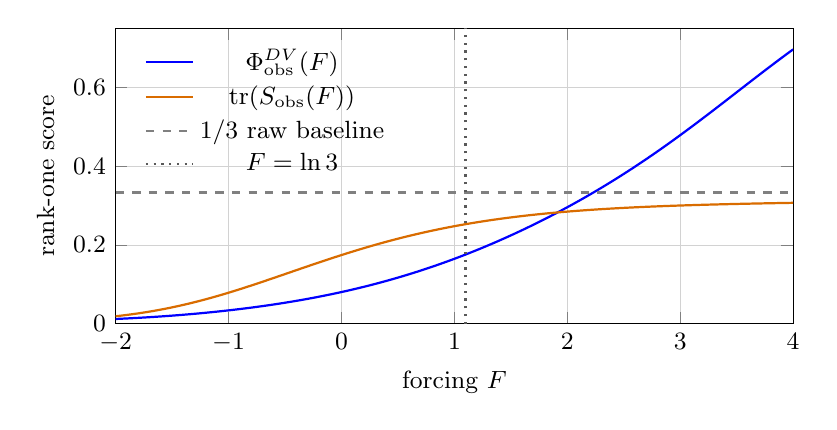
\begin{tikzpicture}
\begin{axis}[
    width=0.84\textwidth,
    height=0.44\textwidth,
    xmin=-2, xmax=4,
    ymin=0, ymax=0.75,
    xlabel={forcing $F$},
    ylabel={rank-one score},
    legend style={draw=none, fill=none, font=\small, at={(0.03,0.97)}, anchor=north west},
    tick label style={font=\small},
    label style={font=\small},
    grid=both,
    grid style={line width=0.1pt, draw=gray!20},
    major grid style={line width=0.2pt, draw=gray!35},
]
\addplot[blue, thick] coordinates { (-2.00,0.012179) (-1.95,0.012831) (-1.90,0.013525) (-1.85,0.014261) (-1.80,0.015040) (-1.75,0.015863) (-1.70,0.016731) (-1.65,0.017643) (-1.60,0.018602) (-1.55,0.019607) (-1.50,0.020660) (-1.45,0.021761) (-1.40,0.022911) (-1.35,0.024112) (-1.30,0.025364) (-1.25,0.026668) (-1.20,0.028026) (-1.15,0.029439) (-1.10,0.030908) (-1.05,0.032434) (-1.00,0.034018) (-0.95,0.035663) (-0.90,0.037368) (-0.85,0.039137) (-0.80,0.040971) (-0.75,0.042870) (-0.70,0.044837) (-0.65,0.046874) (-0.60,0.048982) (-0.55,0.051163) (-0.50,0.053419) (-0.45,0.055751) (-0.40,0.058163) (-0.35,0.060654) (-0.30,0.063229) (-0.25,0.065887) (-0.20,0.068632) (-0.15,0.071466) (-0.10,0.074390) (-0.05,0.077406) (0.00,0.080516) (0.05,0.083722) (0.10,0.087026) (0.15,0.090430) (0.20,0.093935) (0.25,0.097543) (0.30,0.101256) (0.35,0.105074) (0.40,0.109001) (0.45,0.113036) (0.50,0.117181) (0.55,0.121437) (0.60,0.125806) (0.65,0.130287) (0.70,0.134883) (0.75,0.139593) (0.80,0.144419) (0.85,0.149360) (0.90,0.154418) (0.95,0.159592) (1.00,0.164883) (1.05,0.170292) (1.10,0.175818) (1.15,0.181462) (1.20,0.187223) (1.25,0.193103) (1.30,0.199100) (1.35,0.205216) (1.40,0.211451) (1.45,0.217805) (1.50,0.224278) (1.55,0.230871) (1.60,0.237585) (1.65,0.244419) (1.70,0.251376) (1.75,0.258455) (1.80,0.265659) (1.85,0.272987) (1.90,0.280442) (1.95,0.288024) (2.00,0.295735) (2.05,0.303577) (2.10,0.311551) (2.15,0.319659) (2.20,0.327902) (2.25,0.336281) (2.30,0.344799) (2.35,0.353455) (2.40,0.362252) (2.45,0.371190) (2.50,0.380270) (2.55,0.389492) (2.60,0.398855) (2.65,0.408359) (2.70,0.418002) (2.75,0.427784) (2.80,0.437700) (2.85,0.447749) (2.90,0.457925) (2.95,0.468226) (3.00,0.478644) (3.05,0.489174) (3.10,0.499808) (3.15,0.510539) (3.20,0.521357) (3.25,0.532252) (3.30,0.543215) (3.35,0.554233) (3.40,0.565294) (3.45,0.576385) (3.50,0.587494) (3.55,0.598605) (3.60,0.609705) (3.65,0.620778) (3.70,0.631810) (3.75,0.642786) (3.80,0.653691) (3.85,0.664508) (3.90,0.675225) (3.95,0.685826) (4.00,0.696297) };
\addlegendentry{$\Phi_{\mathrm{obs}}^{DV}(F)$}
\addplot[orange!85!black, thick] coordinates { (-2.00,0.019098) (-1.95,0.020725) (-1.90,0.022482) (-1.85,0.024374) (-1.80,0.026405) (-1.75,0.028578) (-1.70,0.030897) (-1.65,0.033364) (-1.60,0.035982) (-1.55,0.038752) (-1.50,0.041675) (-1.45,0.044750) (-1.40,0.047976) (-1.35,0.051352) (-1.30,0.054875) (-1.25,0.058541) (-1.20,0.062347) (-1.15,0.066286) (-1.10,0.070353) (-1.05,0.074541) (-1.00,0.078843) (-0.95,0.083250) (-0.90,0.087755) (-0.85,0.092347) (-0.80,0.097018) (-0.75,0.101758) (-0.70,0.106556) (-0.65,0.111403) (-0.60,0.116287) (-0.55,0.121200) (-0.50,0.126130) (-0.45,0.131068) (-0.40,0.136004) (-0.35,0.140929) (-0.30,0.145833) (-0.25,0.150708) (-0.20,0.155546) (-0.15,0.160338) (-0.10,0.165078) (-0.05,0.169758) (0.00,0.174374) (0.05,0.178917) (0.10,0.183385) (0.15,0.187771) (0.20,0.192072) (0.25,0.196285) (0.30,0.200405) (0.35,0.204430) (0.40,0.208359) (0.45,0.212189) (0.50,0.215918) (0.55,0.219546) (0.60,0.223073) (0.65,0.226497) (0.70,0.229819) (0.75,0.233039) (0.80,0.236157) (0.85,0.239175) (0.90,0.242093) (0.95,0.244913) (1.00,0.247635) (1.05,0.250262) (1.10,0.252794) (1.15,0.255235) (1.20,0.257585) (1.25,0.259847) (1.30,0.262022) (1.35,0.264113) (1.40,0.266123) (1.45,0.268052) (1.50,0.269904) (1.55,0.271681) (1.60,0.273384) (1.65,0.275017) (1.70,0.276582) (1.75,0.278080) (1.80,0.279515) (1.85,0.280887) (1.90,0.282201) (1.95,0.283457) (2.00,0.284659) (2.05,0.285807) (2.10,0.286905) (2.15,0.287954) (2.20,0.288957) (2.25,0.289914) (2.30,0.290829) (2.35,0.291703) (2.40,0.292539) (2.45,0.293336) (2.50,0.294099) (2.55,0.294827) (2.60,0.295524) (2.65,0.296190) (2.70,0.296826) (2.75,0.297435) (2.80,0.298018) (2.85,0.298577) (2.90,0.299111) (2.95,0.299624) (3.00,0.300116) (3.05,0.300587) (3.10,0.301040) (3.15,0.301475) (3.20,0.301894) (3.25,0.302296) (3.30,0.302684) (3.35,0.303058) (3.40,0.303418) (3.45,0.303766) (3.50,0.304102) (3.55,0.304427) (3.60,0.304741) (3.65,0.305045) (3.70,0.305340) (3.75,0.305626) (3.80,0.305903) (3.85,0.306172) (3.90,0.306433) (3.95,0.306687) (4.00,0.306934) };
\addlegendentry{$\operatorname{tr}(S_{\mathrm{obs}}(F))$}
\addplot[gray, dashed, thick] coordinates {(-2,0.333333) (4,0.333333)};
\addlegendentry{$1/3$ raw baseline}
\addplot[gray!70!black, dotted, thick] coordinates {(1.098612,0) (1.098612,0.75)};
\addlegendentry{$F=\ln 3$}
\end{axis}
\end{tikzpicture}
\caption{Observed-link forcing sweep for the edge-induced orthogonal sector $\Pi_{\mathrm{obs}}(F)$ associated with the measured $2\leftrightarrow 3$ link. Blue shows the raw retained fraction $\Phi_{\mathrm{obs}}^{DV}(F)$. Orange shows the shadow trace $\operatorname{tr}(S_{\mathrm{obs}}(F))$. The grey dashed line marks the raw random rank-one baseline $1/3$, and the vertical dotted line marks the benchmark value $F=\ln 3$. The two curves separate visibly, showing that backbone-normalised detectability and raw signal retention are distinct geometric questions even for the same physical observation channel.}
\label{fig:four-state-observed-sector-sweep}
\end{figure}

The worked benchmark shows that the present geometry can compare the actual source observable with the visibility-optimal and detectability-optimal observers, and can track how that gap changes across a physically motivated forcing family.


\subsection{A five-state ribosome proofreading benchmark from the speed-accuracy literature}
\label{sec:banerjee-ribosome-benchmark}

The four-state benchmark shows that the theorem package can compare actual and optimal observers on a standard partial-observation network. We now test the same machinery on a biologically canonical proofreading model. Banerjee, Kolomeisky, and Igoshin analyse aa-tRNA selection by the \emph{E.~coli} ribosome through a five-state kinetic-proofreading network, together with hyperaccurate and error-prone mutants, and argue that the experimentally relevant regime is organised primarily by speed, with energetic proofreading cost as an additional constraint rather than by direct minimisation of error alone \cite{BanerjeeKolomeiskyIgoshin2017}.

To place that system inside the finite-observation framework of the present paper, we use the closed turnover continuous-time Markov model on the state set
\begin{equation}
(E,\,ER,\,ER^{\ast},\,EW,\,EW^{\ast}),
\end{equation}
where \(E\) is the free ribosome, \(ER\) and \(ER^{\ast}\) are the cognate branch before and after hydrolysis, and \(EW\) and \(EW^{\ast}\) are the near-cognate branch before and after hydrolysis. The right-pathway rates and discrimination factors are taken directly from the Banerjee supporting-information tables for the wild type (WT), hyperaccurate mutant (HYP, \(\mathrm{rpsL141}\)), and error-prone mutant (ERR, \(\mathrm{rpsD12}\)) ribosomes \cite{BanerjeeKolomeiskyIgoshin2017}.

As in Banerjee's translation analysis, we impose the nearly irreversible choices \(k_{-2,R}=k_{-3,R}=10^{-3}\,\mathrm{s}^{-1}\) and \(f_{-2}=1\), and derive \(f_{-3}\) from the cycle constraint. The generator used here is not the backward first-passage operator from the source paper. It is the ergodic turnover generator in which both catalytic completion and proofreading reset return the system to the free state \(E\).

Before applying finite observation, we validate the reconstruction against the source biology. The stationary fluxes recover the correct speed and error ordering
\begin{equation}
\text{speed: WT} > \text{HYP} > \text{ERR},
\qquad
\text{error: HYP} < \text{WT} < \text{ERR},
\end{equation}
and the flux-based proofreading cost agrees with the analytic Banerjee formula to relative error below \(2\times 10^{-3}\) for all three variants. The benchmark is a source-locked turnover model that reproduces the intended biological regime before any spectral analysis is performed.

\subsection{Raw spectral concentration and interpretation of effective complexity}

The reduced Fisher tangent space has dimension \(m=4\) for each ribosome variant. Figure~\ref{fig:banerjee-raw-spectrum} and Table~\ref{tab:banerjee-ribosome-summary} show the singular spectrum of the weighted signal operator \(A_{DV}\) and the associated Ky Fan retention hierarchy.

Across all three variants the raw nonequilibrium signal is sharply concentrated. The weighted stable rank lies in the narrow interval
\begin{equation}
1.4130 \leq \operatorname{sr}(A_{DV}) \leq 1.5166,
\end{equation}
while the rank-one retained fractions satisfy
\begin{equation}
0.6594 \leq \Phi^{DV}_{1} \leq 0.7077.
\end{equation}
More importantly, two observer directions already recover almost the entire Donsker-Varadhan correction:
\begin{equation}
\Phi^{DV}_{2}(\mathrm{WT})\approx 0.9867,
\qquad
\Phi^{DV}_{2}(\mathrm{HYP})\approx 0.9913,
\qquad
\Phi^{DV}_{2}(\mathrm{ERR})\approx 0.9504.
\end{equation}
Thus the active signal is effectively rank two in a four-dimensional reduced Fisher space, despite the fact that the underlying proofreading network is multibranch and is usually discussed through several competing biological performance measures. Within the raw finite-observation geometry, the benchmark exhibits a pronounced appearance of spectral simplicity despite topological and functional richness: topological complexity does not imply spectral complexity.

\begin{figure}[t]
\centering
\includegraphics[width=0.98\textwidth]{fig1_raw_spectrum_retention.png}
\caption{Raw weighted-signal spectrum and cumulative Ky Fan retention for the Banerjee ribosome benchmark. For WT, HYP, and ERR, the singular front of \(A_{DV}\) is sharply concentrated. Rank one retains roughly two thirds of the full correction, and rank two retains more than \(95\%\) in every variant.}
\label{fig:banerjee-raw-spectrum}
\end{figure}

\begin{table}[t]
\centering
\caption{Finite-observation summary for the Banerjee ribosome benchmark. The last two columns separate raw concentration from backbone-normalised detectability concentration. Raw rank two suffices for all three variants, whereas the ERR mutant requires full rank to exceed the \(90\%\) detectability threshold.}
\label{tab:banerjee-ribosome-summary}
\begin{tabular}{lcccccc}
\toprule
Variant & \(\operatorname{sr}(A_{DV})\) & \(\Phi^{DV}_{1}\) & \(\Phi^{DV}_{2}\) & \(d_{0.9}^{\mathrm{raw}}\) & \(d_{0.9}^{\mathrm{det}}\) & top \(\theta_k\) \\
\midrule
WT  & 1.4709 & 0.6799 & 0.9867 & 2 & 2 & 0.324613 \\
HYP & 1.4130 & 0.7077 & 0.9913 & 2 & 2 & 0.320700 \\
ERR & 1.5166 & 0.6594 & 0.9504 & 2 & 4 & 0.327211 \\
\bottomrule
\end{tabular}
\end{table}

\subsection{Backbone-normalised detectability and biologically legible observer directions}

The whitened detectability spectrum sharpens the comparison between variants. Figure~\ref{fig:banerjee-detectability} shows that WT and HYP have an almost perfectly rank-two detectability structure: in both cases a nearly degenerate leading pair at
\begin{equation}
\theta_1 \approx \theta_2 \approx 0.32
\end{equation}
dominates, while the residual tail is tiny,
\begin{equation}
\theta_3=\theta_4\approx 0.0062 \quad \text{for WT},
\qquad
\theta_3=\theta_4\approx 0.0026 \quad \text{for HYP}.
\end{equation}
Consequently, two detectability directions already capture more than \(98\%\) of the backbone-normalised signal for WT and HYP. The ERR mutant shows a more mixed geometry. Its leading pair remains dominant,
\begin{equation}
\theta_1 \approx \theta_2 \approx 0.3272,
\end{equation}
but the lower pair remains substantial,
\begin{equation}
\theta_3 \approx \theta_4 \approx 0.1405,
\end{equation}
so rank two captures only about \(70\%\) of detectability and one needs full rank to exceed the \(90\%\) threshold. Raw retention is therefore highly concentrated in all three variants, but detectability distinguishes the speed-optimised WT and HYP variants from the more diffuse ERR mutant.

\begin{figure}[t]
\centering
\includegraphics[width=0.98\textwidth]{fig2_detectability_spectrum.png}
\caption{Backbone-normalised detectability spectrum for the Banerjee ribosome benchmark. WT and HYP are nearly rank two after whitening, while ERR retains a substantial lower pair. This is the clearest place where raw visibility and detectability separate across biologically meaningful variants.}
\label{fig:banerjee-detectability}
\end{figure}

Figure~\ref{fig:banerjee-observer-loadings} shows that the dominant observer directions are also biologically legible. Up to the usual overall sign convention, the top raw observer loads primarily on the cognate branch \(E \leftrightarrow ER \leftrightarrow ER^{\ast}\), while the subdominant direction separates cognate from near-cognate structure. The top detectability observer places its weight mainly on the hydrolysis stage, which is consistent with the role of \(ER \to ER^{\ast}\) as the main distinguishability channel after backbone normalisation and with hydrolysis as the natural discrimination checkpoint of the proofreading cycle. The observer geometry is therefore not only low rank. It is interpretable in terms of the proofreading mechanism itself. As the matched-null comparison later makes clear, however, the resulting low-rank concentration is not by itself specific evidence for proofreading architecture.

\begin{figure}[t]
\centering
\includegraphics[width=0.98\textwidth]{fig4_observer_loadings.png}
\caption{Top raw and top detectability observer loadings for WT, HYP, and ERR. The labels \(E\), \(ER\), \(ER^{\ast}\), \(EW\), and \(EW^{\ast}\) denote the free, cognate pre-hydrolysis, cognate post-hydrolysis, near-cognate pre-hydrolysis, and near-cognate post-hydrolysis states. Overall signs are conventional. The dominant directions remain concentrated on biologically recognisable proofreading coordinates rather than on diffuse mixtures of all states.}
\label{fig:banerjee-observer-loadings}
\end{figure}

\subsection{Robustness under hydrolysis-rate variation}

Banerjee's own speed-accuracy analysis identifies the hydrolysis step as a key kinetic control axis for the WT ribosome \cite{BanerjeeKolomeiskyIgoshin2017}. We therefore perform a one-parameter finite-observation sweep over \(k_{2,R}\) while keeping the remaining WT parameters fixed. Figure~\ref{fig:banerjee-k2r-sweep} shows that the low-rank picture is robust across this family. The rank-one retained fraction stays above \(0.66\), the rank-two retained fraction stays above \(0.969\), the weighted stable rank remains close to \(1.5\), and the top detectability eigenvalue rises smoothly toward a plateau near \(0.33\). Across the hydrolysis-rate sweep, the dominant detectability structure remains low-rank and varies smoothly. There is no sharp spectral transition in the biologically relevant band. The spectral simplicity of the WT proofreading network is therefore a structural feature of the benchmark family, not a knife-edge artefact of one fitted parameter set.

\begin{figure}[t]
\centering
\includegraphics[width=0.84\textwidth]{fig5_parameter_sweep_k2R.png}
\caption{WT hydrolysis-rate sweep for the Banerjee ribosome benchmark. The raw rank-one retained fraction, raw rank-two retained fraction, weighted stable rank, and top detectability eigenvalue remain in a narrow low-rank regime across the relevant range of \(k_{2,R}\). The dashed vertical line marks the WT value from the source model.}
\label{fig:banerjee-k2r-sweep}
\end{figure}

Taken together, the Banerjee benchmark upgrades the theorem package from a compact literature network to a biologically canonical proofreading system with experimentally grounded parameters and variant structure. The conclusion is unusually clean. A network that is functionally rich enough to support speed-accuracy-cost trade-off analysis can still be spectrally simple in the finite-observation geometry. In this benchmark, most of the nonequilibrium correction lives in two observer directions, and the remaining distinction between variants becomes visible only after backbone whitening.

\subsection{A matched random null for the Banerjee benchmark}

The Banerjee ribosome benchmark is useful, but its structural interpretation must be stated carefully. We therefore compare the WT proofreading network against a matched null ensemble of dense random five-state nonequilibrium CTMCs with the same mean exit-rate scale and with total DV energy restricted to a narrow band around the real benchmark. The null ensemble was designed to answer a specific question: is the strong raw rank-two compression in the ribosome case a special fingerprint of proofreading architecture, or is it largely a dimensional effect of working in a four-dimensional reduced Fisher space?

This random-ensemble perspective is also consonant with recent work showing that, in broad classes of random Markov models, many irreversibility-sensitive observables are controlled primarily by heterogeneity rather than by asymmetry alone except near symmetry \cite{MosamDeGiuli2026}.

The answer is the latter. As Figure~\ref{fig:banerjee-negative-control} shows, across the primary raw metrics the real Banerjee WT point sits close to the middle of the matched null distribution rather than in an extreme low-rank tail. In particular,
\begin{equation}
\Phi^{DV}_{1}(\mathrm{WT})\approx 0.6799,
\qquad
\Phi^{DV}_{2}(\mathrm{WT})\approx 0.9867,
\qquad
\operatorname{sr}(A_{DV})\approx 1.4709,
\end{equation}
so the WT point sits close to the middle of the sampled null ensemble on all three raw metrics. Thus the Banerjee network remains an important demonstration that the finite-observation machinery can be applied to a real biochemical system with biologically legible observer directions, but the raw low-rank compression itself cannot be claimed as a special consequence of proofreading architecture.

\begin{figure}[t]
\centering
\includegraphics[width=0.86\textwidth]{neg_fig1_null_distributions.png}
\caption{Matched random null for the Banerjee ribosome benchmark. The WT proofreading network lies near the centre of the null distribution for the main raw concentration measures once the total DV scale is matched. The benchmark therefore remains useful as a biologically interpretable worked example, but its strong raw rank-two concentration is not by itself evidence for a proofreading-specific structural simplification.}
\label{fig:banerjee-negative-control}
\end{figure}


\subsection{A force-driven kinesin benchmark from the molecular-motor literature}
\label{sec:kinesin-benchmark}

To test whether the same spectral compression extends beyond proofreading, we next turn to the chemomechanical kinesin model of Liepelt and Lipowsky \cite{LiepeltLipowsky2007,LiepeltLipowsky2007Supp}. This benchmark is mechanistically distinct from the Banerjee ribosome network. Its primary form is a six-state motor with two competing chemomechanical cycles and one purely dissipative cycle, together with explicit load-force control through a mechanical load-distribution factor and force-sensitive chemical prefactors. The supplement also gives a reduced seven-state small-load extension in which a doubly ADP-bound state opens an additional forward cycle. We use the source-locked six-state model at arbitrary load, and the reduced seven-state model only in the zero-load regime where the source supplement explicitly justifies that truncation and supplies the extra rates.

For the six-state model the transition rates are built in the source convention as
\begin{equation}
\omega_{ij}=\kappa_{ij}\,I_{ij}([ATP],[ADP],[P])\,\Phi_{ij}(F),
\end{equation}
with rate constants from Table~I of \cite{LiepeltLipowsky2007}, force parameters from Table~II and Appendix~A of \cite{LiepeltLipowsky2007Supp}, and the backward-cycle rate \(\kappa_{54}=(\kappa_{52}/\kappa_{25})^2\kappa_{21}\) imposed as in the source derivation. The reduced seven-state model retains only the additional edges \(1\leftrightarrow 7\) and \(5\leftrightarrow 7\), again as prescribed in Appendix~D of \cite{LiepeltLipowsky2007Supp}. 

Before applying finite observation, we validate the reconstruction against the source dynamics: both force-data parametrisations reproduce a stall force near \(7.2\,\mathrm{pN}\), the six-state model reproduces the source asymmetry between \([P]\)- and \([ADP]\)-dependence at zero load, and the reduced seven-state model restores the missing high-ADP slowdown while producing the predicted crossover to the added \(F_{DD}\) cycle at \([ADP]\approx 1083\,\mu\mathrm{M}\).

\subsection{Raw concentration across force and concentration}

The six-state kinesin benchmark is sharply low-rank across the tested regimes. At zero load, all three published source parametrisations are essentially rank one in the raw Donsker--Varadhan correction:
\begin{equation}
\Phi^{DV}_{1}(\mathrm{[15]},F=0)\approx 0.9777,
\qquad
\Phi^{DV}_{1}(\mathrm{[9]},F=0)\approx 0.9988,
\qquad
\Phi^{DV}_{1}(\mathrm{[12]},F=0)\approx 0.9563,
\end{equation}
with weighted stable rank in the narrow interval
\begin{equation}
1.0012 \le \operatorname{sr}(A_{DV}) \le 1.0457.
\end{equation}
Thus a single observer direction already captures more than \(95\%\) of the nonequilibrium correction in every zero-load case.

Figure~\ref{fig:kinesin-raw-force} shows how this picture evolves under load for the two source force-data parametrisations. Broadening does occur near stall, but it is physically transparent rather than pathological. For the [15] fit, rank-one retention drops from \(0.9777\) at zero load to about \(0.5260\) near \(7\,\mathrm{pN}\), while the weighted stable rank rises from \(1.0228\) to \(1.9012\). 

For the [9] fit, the broadening is milder, with \(\Phi_1^{DV}\approx 0.6462\) and \(\operatorname{sr}(A_{DV})\approx 1.5474\) at \(7\,\mathrm{pN}\). In both cases, however, the low-rank tendency persists away from the stall region. This is the behaviour one would expect if the singular front is controlled by the competition between forward and backward chemomechanical cycles: the spectrum is narrow when one cycle dominates and broadens only when the cycle currents come close to balance.

\begin{figure}[t]
\centering
\includegraphics[width=0.98\textwidth]{fig1_6state_raw_spectrum_force.png}
\caption{Six-state kinesin benchmark under force. Left panels: singular values of the weighted signal operator \(A_{DV}\) for the [15] and [9] source fits. Middle panels: cumulative raw Ky Fan retention fractions \(\Phi_1^{DV}\) and \(\Phi_2^{DV}\). Right panels: weighted stable rank. The signal is almost rank one at low load and broadens only near stall, where the forward and backward chemomechanical cycles compete most strongly.}
\label{fig:kinesin-raw-force}
\end{figure}

The zero-load concentration stress test in Figure~\ref{fig:kinesin-concentration} shows a second important feature. The six-state geometry is almost insensitive to \([P]\), for which the source paper already reports good kinetic agreement, while \([ADP]\) produces only a mild spectral shift even in the regime where the six-state velocity law is known to underpredict the slowdown. For the [12] parametrisation at \(F=0\), the raw rank-one retained fraction stays near \(0.956\) throughout the \([P]\)-sweep and rises only slightly, from about \(0.958\) to \(0.967\), over four decades of \([ADP]\). Thus the kinetic failure of the six-state model at high ADP is not a failure of raw spectral concentration.

\begin{figure}[t]
\centering
\includegraphics[width=0.98\textwidth]{fig3_6state_conc_stress_test.png}
\caption{Zero-load concentration stress test for the six-state kinesin model using the [12] source parametrisation. The \([P]\)-sweep leaves the raw singular spectrum and cumulative retention almost unchanged. The \([ADP]\)-sweep produces a mild increase in concentration while the reference velocity falls strongly, matching the source observation that the six-state model captures the phosphate trend but underestimates the ADP slowdown.}
\label{fig:kinesin-concentration}
\end{figure}

\subsection{Backbone-normalised detectability and the reduced seven-state extension}

The whitened detectability spectrum is materially broader than the raw spectrum. Figure~\ref{fig:kinesin-detectability} shows that the top detectability eigenvalue remains of order \(10^{-2}\) to \(10^{-1}\), but the detectability mass is spread over more directions than the raw DV correction. In the representative six-state cases of Table~\ref{tab:kinesin-summary}, one typically needs rank four to exceed the \(90\%\) detectability threshold even when the raw signal is already more than \(95\%\) concentrated in rank one. This reproduces, in a mechanochemically different system, the same separation between raw visibility and backbone-normalised detectability that was already visible in the ribosome benchmark.

\begin{figure}[t]
\centering
\includegraphics[width=0.98\textwidth]{fig2_6state_detectability_force.png}
\caption{Backbone-normalised detectability for the six-state kinesin benchmark under force. Detectability is substantially broader than the raw weighted signal, and the broadening becomes strongest near stall. The theory therefore distinguishes raw nonequilibrium visibility from statistical distinguishability against the detailed-balance backbone even within the same molecular-motor family.}
\label{fig:kinesin-detectability}
\end{figure}

The reduced seven-state model strengthens the cross-model recurrence case further. Its purpose in the source literature is to repair the missing \([ADP]\)-dependence of the six-state motor by adding a doubly ADP-bound state and the corresponding forward cycle \(F_{DD}^{+}=|12571\rangle\). In the finite-observation geometry, however, the added mechanistic structure does not broaden the signal. Figure~\ref{fig:kinesin-7state-adp} shows that the rank-one retained fraction actually increases with \([ADP]\), from about \(0.9560\) at \(1\,\mu\mathrm{M}\) to \(0.9740\) at \(5000\,\mu\mathrm{M}\), while the weighted stable rank falls from \(1.0460\) to \(1.0267\). At the same time, the top detectability eigenvalue decreases from \(6.24\times 10^{-2}\) to \(2.82\times 10^{-2}\), and the minimal detectability rank for \(90\%\) retention improves from four to two. The source paper's extra cycle becomes dynamically important without destroying the low-rank observer geometry.

\begin{figure}[t]
\centering
\includegraphics[width=0.98\textwidth]{fig4_7state_ADP_sweep.png}
\caption{Reduced seven-state kinesin benchmark at zero load under an \([ADP]\) sweep. The added doubly ADP-bound state and cycle \(F_{DD}^{+}=|12571\rangle\) improve the source kinetic fit at high ADP, but they do not broaden the finite-observation geometry. Raw rank-one retention increases, the stable rank falls slightly, and detectability becomes easier to compress at large ADP.}
\label{fig:kinesin-7state-adp}
\end{figure}

\begin{table}[t]
\centering
\caption{Representative finite-observation summary for the kinesin benchmark. Raw rank-one concentration is already extreme at low load and remains strong in the reduced seven-state extension. Detectability is broader than raw visibility in the six-state motor but becomes easier to compress in the high-ADP seven-state regime.}
\label{tab:kinesin-summary}
\begin{tabular}{lccccccc}
\toprule
Case & \(n\) & \(\Phi^{DV}_{1}\) & \(\Phi^{DV}_{2}\) & \(\operatorname{sr}(A_{DV})\) & top \(\theta_{1}\) & \(d^{\mathrm{raw}}_{0.9}\) & \(d^{\mathrm{det}}_{0.9}\) \\
\midrule
6s,[15], \(F=0\) & 6 & 0.9777 & 0.9911 & 1.0228 & 0.0623 & 1 & 4 \\
6s,[15], \(F=7\,\mathrm{pN}\) & 6 & 0.5260 & 0.8695 & 1.9012 & 0.0465 & 3 & 4 \\
6s,[9], \(F=0\) & 6 & 0.9988 & 0.9995 & 1.0012 & 0.0623 & 1 & 4 \\
6s,[12], \(F=0\) & 6 & 0.9563 & 0.9825 & 1.0457 & 0.0624 & 1 & 4 \\
7s,[12], \([ADP]=5000\,\mu\mathrm{M}\) & 7 & 0.9740 & 0.9966 & 1.0267 & 0.0282 & 1 & 2 \\
\bottomrule
\end{tabular}
\end{table}

Figure~\ref{fig:kinesin-observer-loadings} shows that the leading observer directions remain structured rather than diffuse. In the six-state family, the dominant raw and detectability directions concentrate on only a few numbered states at a time, and in the seven-state ADP regime the new state 7 enters coherently rather than spreading weight uniformly across the enlarged network. This again points to a low-dimensional active nonequilibrium core rather than to generic high-dimensional mixing.

\begin{figure}[t]
\centering
\includegraphics[width=0.98\textwidth]{fig5_observer_loadings.png}
\caption{Leading raw and detectability observer loadings for representative six-state and reduced seven-state kinesin operating points in the canonical numbered state basis. Overall signs are conventional. The dominant directions remain concentrated on a small number of states and reorganise coherently as load or ADP changes, rather than diffusing across the full state graph.}
\label{fig:kinesin-observer-loadings}
\end{figure}

Taken together, the kinesin benchmark materially strengthens the case for cross-model recurrence. The Liepelt--Lipowsky motor is not a proofreading network. It has competing chemomechanical cycles, explicit load-force control, and, in the reduced seven-state extension, a third forward cycle that becomes dominant at high ADP. Yet the finite-observation geometry is at least as concentrated as in the Banerjee ribosome benchmark across most of the tested regimes. The one place where concentration weakens, near stall, is physically transparent: it is exactly where the forward and backward motor cycles come closest to balance. This is therefore not a failure of the low-rank theory but one of its clearest mechanistic confirmations.


\subsection{Matched negative controls for the kinesin motor benchmark}

Unlike the Banerjee benchmark, the kinesin benchmark behaves differently. Here the positive result survives matched negative controls. We compare three real operating points against graph-matched nonequilibrium control ensembles: anchor A, the six-state motor at zero load; anchor B, the same six-state model near stall; and anchor C, the reduced seven-state model at zero load and high ADP. Two control classes are used. NC1 keeps the graph but replaces the structured motor rates by random positive rates. NC2 is stricter: it keeps the graph and approximately matches the stationary law while randomising the nonequilibrium edge asymmetry.

At the two main low-rank anchors, the real motor is substantially more concentrated than the controls, as shown in Figure~\ref{fig:kinesin-negative-controls}. For anchor A the real six-state motor has
\begin{equation}
\Phi^{DV}_{1}\approx 0.9777,
\qquad
\operatorname{sr}(A_{DV})\approx 1.0228,
\end{equation}
placing it above all sampled NC1 controls and above most sampled values in the stricter $\pi$-matched NC2 ensemble. For anchor C the reduced seven-state model has
\begin{equation}
\Phi^{DV}_{1}\approx 0.9740,
\qquad
\operatorname{sr}(A_{DV})\approx 1.0267,
\end{equation}
placing it above nearly all sampled NC1 controls and above most sampled NC2 controls. Thus the low-rank concentration is not a generic consequence of graph size or edge count alone, and it is only partly explained by the stationary-law profile.

The one exception is the near-stall anchor B, which is now taken at the same \(F=7\,\mathrm{pN}\) operating point reported in Table~\ref{tab:kinesin-summary}. At this anchor the real motor becomes \emph{less} concentrated than the matched random controls, with
\begin{equation}
\Phi^{DV}_{1}\approx 0.5260,
\qquad
\operatorname{sr}(A_{DV})\approx 1.9012,
\end{equation}
placing the real point below most sampled random controls. The qualitative conclusion is unchanged but now better calibrated: near stall the real motor is less concentrated than typical controls, though not pathologically so. This is the regime in which the forward and backward chemomechanical cycles compete most strongly. The negative control sharpens the mechanistic reading of the benchmark by identifying the stall region as the place where low-rank concentration weakens.

\begin{figure}[t]
\centering
\includegraphics[width=0.88\textwidth]{neg_fig_nc_5_retention_curves.png}
\caption{Kinesin matched negative controls. The red curves are the real motor benchmarks and the blue bands are graph-matched control ensembles. At the zero-load six-state anchor and the high-ADP seven-state anchor, the real motor retains substantially more DV signal in low observer rank than the controls. Near stall, the situation reverses: the real motor broadens more strongly than the controls, consistent with direct competition between forward and backward chemomechanical cycles.}
\label{fig:kinesin-negative-controls}
\end{figure}

Taken together, the negative controls sharpen the interpretation of both biological examples. For the Banerjee ribosome, the benchmark is valuable mainly as an experimentally grounded and biologically interpretable worked example, but not as evidence that proofreading architecture is unusually low-rank. For kinesin, by contrast, the control ensembles show that the observed spectral compression is not generic to comparable nonequilibrium graphs. The molecular-motor result therefore provides the stronger empirical support for a nontrivial cross-model recurrence claim.



\subsection{A ten-state chemotaxis feedback benchmark from the sensory-adaptation literature}
\label{sec:sartori-chemotaxis-benchmark}

The kinesin benchmark shows that strong finite-observation compression can survive outside proofreading and across explicit motor-force control. We now test a larger sensory-feedback system. Sartori, Granger, Lee, and Horowitz study \emph{E.~coli} chemotaxis through a ten-state receptor model with two activity states \(a\in\{0,1\}\) and five methylation levels \(m\in\{0,1,2,3,4\}\), maintained out of equilibrium by SAM-driven methylation \cite{SartoriGrangerLeeHorowitz2014}. At fixed ligand concentration \([L]\), the state space is
\begin{equation}
(a,m)\in\{0,1\}\times\{0,1,2,3,4\},
\end{equation}
ordered in the implementation as
\begin{equation}
(0,0),(1,0),(0,1),(1,1),(0,2),(1,2),(0,3),(1,3),(0,4),(1,4).
\end{equation}
The source kinetics are fixed by the Tar receptor parameters
\begin{equation}
K_I=18.2\,\mu\mathrm{M},\qquad K_A=3000\,\mu\mathrm{M},\qquad
\Delta_m=2,\qquad m_0=1,
\end{equation}
together with the separated timescales
\begin{equation}
\tau_a=10^{-3}\,\mathrm{s},\qquad \tau_m=10\,\mathrm{s},
\end{equation}
and chemical driving
\begin{equation}
\Delta\mu=6\,k_B T.
\end{equation}
We build the fixed-ligand generator directly from the source rate formulas for activity flips and nearest-neighbour methylation moves, and evaluate it at
\begin{equation}
[L]\in\{94,200,500,720,1500,3000,5760\}\,\mu\mathrm{M},
\end{equation}
which spans the adaptive regime \(K_I\ll [L]\ll K_A\), its upper edge, and the strongly saturated outside region \cite{SartoriGrangerLeeHorowitz2014}.

Before any spectral analysis, we impose the same source-locking standard used in the previous biological examples. The implemented generator reproduces the ten-state receptor graph of the source model, including all horizontal activity flips and all vertical nearest-neighbour methylation transitions. Local detailed balance holds on the activity sector by construction, and the SAM-driven methylation asymmetry breaks detailed balance at every tested ligand value. The resulting stationary laws are positive and normalised. They also reproduce a key qualitative feature of the source paper: the methylation marginal remains heavily concentrated at the highest methylation level, with Bhattacharyya overlaps above \(0.999\) across representative ligand pairs. Thus the benchmark is not an abstract ten-state toy. It is a source-locked receptor model in the specific high-methylation operating regime used by Sartori \emph{et al.} to discuss the limited memory capacity of the feedback architecture.

\begin{figure}[t]
\centering
\includegraphics[width=0.98\textwidth]{Sartori_fig1_raw_spectrum.png}
\caption{Raw weighted-signal spectrum and cumulative Ky Fan retention for the Sartori ten-state chemotaxis benchmark. Across all tested ligand concentrations, the weighted signal operator \(A_{DV}\) has a sharply dominant singular front. One observer direction captures about \(85\%\) to \(97\%\) of the raw DV signal, and two directions capture at least about \(99.5\%\).}
\label{fig:sartori-raw-spectrum}
\end{figure}

The raw Donsker--Varadhan correction is sharply concentrated across the entire ligand family, as shown in Figure~\ref{fig:sartori-raw-spectrum}. In the adaptive regime, the one-direction retained fraction is already
\begin{equation}
\Phi_1^{DV}\approx 0.972 \quad \text{at } [L]=94\,\mu\mathrm{M},
\end{equation}
with
\begin{equation}
\Phi_2^{DV}\approx 0.999,\qquad \operatorname{sr}(A_{DV})\approx 1.029.
\end{equation}
Even at the largest tested ligand concentration,
\begin{equation}
[L]=5760\,\mu\mathrm{M},
\end{equation}
well beyond \(K_A\), the signal remains strongly compressed:
\begin{equation}
\Phi_1^{DV}\approx 0.850,\qquad
\Phi_2^{DV}\approx 0.995,\qquad
\operatorname{sr}(A_{DV})\approx 1.176.
\end{equation}
Thus a ten-state sensory-feedback network with a nine-dimensional reduced Fisher space still behaves, in raw finite-observation geometry, almost as a rank-one system. This is materially stronger than the Banerjee proofreading example, where an analogous low-rank conclusion could still be questioned as a small-state-space effect.

\begin{figure}[t]
\centering
\includegraphics[width=0.98\textwidth]{Sartori_fig2_detectability_spectrum.png}
\caption{Backbone-normalised detectability spectrum for the Sartori chemotaxis benchmark. Raw visibility is almost rank one throughout the ligand family, but detectability is broader: the leading whitened eigenmodes retain most, but not all, of the concentration. This is the same structural separation between raw nonequilibrium signal and backbone-normalised distinguishability already seen in the ribosome and kinesin benchmarks.}
\label{fig:sartori-detectability-spectrum}
\end{figure}

As in the previous worked examples, raw visibility and backbone-normalised detectability do not coincide, as shown in Figure~\ref{fig:sartori-detectability-spectrum}. The top detectability eigenvalue rises from about
\begin{equation}
\theta_1\approx 6.68\times 10^{-6}
\end{equation}
at \(94\,\mu\mathrm{M}\) to a peak near
\begin{equation}
\theta_1\approx 3.86\times 10^{-5}
\end{equation}
around \(3000\,\mu\mathrm{M}\), while the detectability stable rank grows from about \(2.14\) to \(3.00\) in the present backbone-normalised scaling. In cumulative terms, one raw direction suffices for \(90\%\) retention over most of the adaptive regime, whereas the backbone-whitened concentration typically requires two to four directions. The chemotaxis benchmark therefore reinforces, in a mechanistically different setting, the main message of Section~\ref{sec:shadow-operator-gaussian-distinguishability}: the visible signal and the statistically distinguishing signal against the detailed-balance backbone are related, but they are not the same geometric object.

\begin{figure}[H]
\centering
\includegraphics[width=0.92\textwidth]{Sartori_fig3_observer_loadings.png}
\caption{Leading raw and detectability observer loadings for the Sartori ten-state chemotaxis benchmark in the ordered basis \((0,0),(1,0),(0,1),(1,1),(0,2),(1,2),(0,3),(1,3),(0,4),(1,4)\). Blue bars denote inactive states and red bars active states. Overall signs are conventional. The dominant raw observer remains a low-methylation activity contrast across the ligand range, while the detectability-optimal observer varies more strongly with ligand concentration.}
\label{fig:sartori-observer-loadings}
\end{figure}

The leading observer directions remain interpretable rather than diffuse. Figure~\ref{fig:sartori-observer-loadings} shows that the dominant raw observer is concentrated almost entirely on the lowest methylation level, as an activity contrast between \((0,0)\) and \((1,0)\), with only a small secondary correction at \(m=1\). The detectability-optimal direction is broader and more ligand-dependent: in some regimes it is dominated by the inactive low-methylation state \((0,0)\), in others by the active low-methylation state \((1,0)\), with smaller balancing weight on \((0,1)\) or \((1,1)\). This is the pattern one expects when the raw nonequilibrium correction is nearly rank one but the detailed-balance backbone is anisotropic.

	\begin{figure}[H]
	\centering
	\includegraphics[width=0.95\textwidth]{Sartori_fig4_ligand_sweep.png}
	\caption{Ligand sweep for the Sartori ten-state chemotaxis benchmark. The green band marks the adaptive regime \(K_I\ll [L]\ll K_A\). Top left: \(\Phi_1^{DV}\) and \(\Phi_2^{DV}\). Top right: weighted stable rank. Bottom left: top detectability eigenvalue. Bottom right: total DV signal energy. The raw concentration is sharpest inside the adaptive regime and degrades only gradually outside it, while the total DV signal grows monotonically and saturates above \(K_A\).}
	\label{fig:sartori-ligand-sweep}
	\end{figure}

The continuous ligand sweep in Figure~\ref{fig:sartori-ligand-sweep} makes the operating-point dependence clear. Inside the adaptive window, the raw signal is most concentrated:
\begin{equation}
\Phi_1^{DV}\approx 0.97,\qquad \operatorname{sr}(A_{DV})\approx 1.03.
\end{equation}
As \([L]\) rises through and beyond \(K_A\), the rank-one retained fraction decays smoothly toward about \(0.79\), while \(\Phi_2^{DV}\) remains close to \(0.99\), the weighted stable rank rises only to about \(1.27\), and the total DV signal energy grows monotonically before saturating. There is no sharp spectral transition at the edge of the adaptive regime. The geometry changes gradually with ligand level rather than catastrophically.

\begin{figure}[H]
\centering
\includegraphics[width=0.92\textwidth]{Sartori_fig5_methylation_validation.png}
\caption{Validation against the source methylation-distribution picture. The stationary methylation marginal is heavily concentrated at \(m=4\) for both in-regime and out-of-regime ligand pairs, with Bhattacharyya overlaps above \(0.999\). This reproduces the source paper's limited-memory observation and shows that the finite-observation signal concentration is extracted on top of, rather than instead of, the high-overlap methylation statistics.}
\label{fig:sartori-methylation-validation}
\end{figure}

The methylation validation in Figure~\ref{fig:sartori-methylation-validation} is important for interpretation. The source model operates in a regime where the stationary methylation marginals remain extremely similar across ligand values, even when the mean activity changes appreciably. The finite-observation result is therefore not that the methylation memory is broad and low-rank. It is subtler. The raw nonequilibrium correction is sharply concentrated even though the methylation marginals themselves are almost indistinguishable. This explains why the dominant observer localises on a low-methylation activity contrast rather than on a broad redistribution over all methylation levels.

Taken together, the Sartori benchmark strengthens the empirical recurrence case in a more demanding state space than Banerjee. The model is mechanistically distinct from both proofreading and chemomechanical transport, and its reduced Fisher space has dimension nine rather than four or five. Yet the raw finite-observation geometry remains strongly compressed throughout the tested ligand family. At the same time, the benchmark preserves the same structural lesson already seen in the earlier biological examples: detectability is broader than raw visibility, and the leading observer directions remain physically interpretable. The correct conclusion is therefore not that every aspect of chemotactic memory is low-dimensional. It is that, in this source-locked ten-state feedback receptor model, the Donsker--Varadhan correction itself has a sharply concentrated spectral front. What remains open for this benchmark is a matched-null control family comparable to the kinesin negative-control analysis; until that is in hand, the chemotaxis example should be read as a source-locked worked example rather than as evidence that sensory-feedback architecture generically enforces low rank.


\section{Related-work connections}
\label{sec:related-work-connections}

\subsection{Estimators, hidden events, and coarse observation}

A large part of the partial-observation literature studies estimator quality, lower bounds, hidden events, unresolved transitions, and coarse-graining schemes for irreversibility detection \cite{BaiesiNishiyamaFalasco2023,BlomSongVougaGodecMakarov2025,FritzErtelSeifert2024,Harunari2024,vanderMeerSaito2025,ErtelSeifert2025,Ehrich2021,DeguntherVanDerMeerSeifert2024,MeybergDeguntherSeifert2024,RoldanParrondo2012}. Those works ask how much irreversibility can be inferred from restricted data.

The present paper addresses a complementary question. Alongside asking which estimator is best, one can ask how much nonequilibrium signal the chosen observable sector can retain in principle. In the regime treated here, that question is governed by a weighted spectral envelope, its hidden share is the spectral tail, and observer quality is controlled by alignment with the singular front of the correction. The Gaussian shadow divergences studied here are local observed-Gaussian comparison laws, conceptually adjacent to trajectory-level irreversibility measures such as Rold\'an--Parrondo, but not the same object.

\subsection{Observer dependence, coarse graining, and design}

Restricted-information and coarse-grained thermodynamic frameworks emphasise that observation is part of the thermodynamic problem itself \cite{RubinoBruknerManzano2025,PernambucoCeleri2026,vanderMeerSaito2025,TezaStellaGrandPre2025,TezaStella2020}. Work on current fluctuations, random counting observables, and optimised coarse-graining schemes makes the same point from a design perspective: some observations are much better than others for irreversibility detection \cite{GingrichRotskoffHorowitz2017,BaoOhgaIto2025,YuLeightonLynn2025}.

The alignment and shadow theorems make that statement concrete in the present setting. A visibility-optimal observer aligns with the singular front of the raw signal. A detectability-optimal observer aligns with the singular front of the backbone-whitened signal. The theory therefore gives a geometric ranking of observers rather than only a qualitative statement that coarse observation can help or hurt.

\subsection{Conceptual and geometric context}

Several neighbouring literatures sharpen the conceptual space. Frenesy and time-symmetric dynamical activity make clear that nonequilibrium structure is richer than entropy-production rates alone \cite{Maes2020}. Conditioned-process theory shows how distinct microscopic dynamics can collapse onto equivalent effective descriptions under large-deviation tilts \cite{ChetriteTouchette2015}.

Spectral work on nonreversible chains shows that singular-value and gap objects can carry operational content rather than serving as linear-algebraic decoration; in the present context such gap control helps set the scale of the detailed-balance backbone against which the weighted signal is read \cite{Chatterjee2025}. The cycle-current perspective of Schnakenberg and Andrieux--Gaspard clarifies the physical source of the skew sector, while reversible-chain information geometry provides a natural detailed-balance backdrop for the Fisher-coordinate formulation used here \cite{Schnakenberg1976,AndrieuxGaspard2007,WolferWatanabe2021}. We also note a nearby geometric literature around Souriau's Lie-group thermodynamics and Barbaresco's Souriau-Fisher information geometry \cite{Souriau1997,Barbaresco2016,Barbaresco2018}.

Taken together, these neighbouring literatures locate the results clearly. The paper is complementary to work on bounds, estimators, and coarse-grained thermodynamics. Its specific contribution is a finite-dimensional visibility law for the Donsker--Varadhan correction in the Markov Gaussian regime, together with its observer geometry, shadow criterion, and ordered spectral readout.

\section{Scope}
\label{sec:scope-falsifiers-outlook}

\subsection{What is proved}

Within this setting, the Donsker--Varadhan correction is identified as a positive weighted correction operator generated by the reduced skew channel and factorising through the weighted signal operator and the detailed-balance backbone. Within its stated Gaussian and orthogonal-observer scope, the theory gives the visibility law, the full envelope hierarchy, retention fractions, hidden tail, stable-rank obstruction, alignment formula, optimal and generic orthogonal observers, the shadow formulas, and the backbone-whitened detectability reformulation. In particular, the envelope hierarchy determines the eigenvalue profile of \(\Delta_{DV}\), equivalently the singular-energy profile \(\tfrac14 s_k(A_{DV})^2\), while the shadow hierarchy supplies the distinct spectrum relevant for Gaussian distinguishability.

The abstract weighted-geometry theorem also holds in finite dimension. It is a transfer theorem: once a positive semidefinite correction admits a weighted Gram factorisation relative to a positive-definite metric, the envelope, alignment, visibility hierarchy, and spectral-readout machinery transfer by Euclideanisation. This includes BKM-symmetrised operator space.

It is equally important to state what is not proved here. Projection suppression and shared observed-Gaussian behaviour are asymptotic Gaussian corollaries, not new bridge theorems. The exact separation proved here is a Hessian-level statement, and beyond quadratic order the paper does not rule out mixed dissipative-skew terms in the full rate function. The linear quantum extension is only at the level of weighted geometry transfer. It is therefore a conditional geometric framework rather than a tested model-specific theory, since no concrete quantum correction operator with the required structure is exhibited here. The full nonlinear quantum fluctuation bridge remains open.

\subsection{Falsification}

At the classical bridge level, the theory would fail if the reduced-coordinate correction were not representable as a weighted Gram signal built from the skew sector and the detailed-balance backbone. Numerically, the bridge claim fails if a direct computation gives \(\|\Delta_{DV}-\tfrac14\widehat J H_0^{-1}\widehat J^T\|\) above tolerance. The bridge identity is therefore a genuine key step.

At the finite-observation level, the envelope law would fail if direct optimisation over orthogonal rank-\(d\) projectors did not agree with the singular-energy formula for \(K_d^{DV}\), or if finite observation in the relevant fluctuation geometry were not correctly modelled by orthogonal compression on the reduced Euclidean Fisher space. In other words, if the physically relevant observable sectors could not be represented in this way, then the visibility law would no longer be the correct model.

At the statistical level, the Gaussian shadow package fails if KL, Hellinger, or total-variation quantities computed directly from the compressed Gaussian covariances do not match the spectral formulas in the shadow operator. At the same time, the equilibrium-shadow theorem is only a Gaussian theorem. It would be falsified as a general statement about observed nonequilibrium if the relevant finite-observation signatures in a given system were dominated by strongly non-Gaussian effects outside the quadratic regime, even when the projected Hessian correction is small.

At the spectroscopy level, the claim fails if the envelope increments do not reproduce the nonzero spectrum of \(\Delta_{DV}\), or if the \(H_0\)-whitened Ky Fan values do not agree with the generalised-eigenvalue detectability spectrum.

Finally, the operator-space extension would fail as a physical theory if no meaningful linear fluctuation correction in BKM geometry could be identified for the relevant quantum nonequilibrium setting. The weighted transfer theorem would remain mathematically true, but it would lose physical force.

\subsection{What the worked examples support, and what they do not}

The worked examples play a calibrating role. They show that the distinction between raw visibility and backbone-normalised detectability remains informative across mechanistically distinct nonequilibrium models. In this empirical arc, the ribosome benchmark provides utility together with restraint, because the matched null shows that low-rank concentration in a small five-state system should not by itself be read as architecture-specific specialness. The kinesin benchmark is the stronger cross-domain recurrence case: it shows robust low-rank concentration at low load together with physically sensible broadening near stall under direct cycle competition. The chemotaxis benchmark is the larger-state-space stress test: it indicates that the same operator theory can remain informative beyond the smallest reduced spaces.

At the same time, the examples do not yet prove a universal low-rank law definitively. They support repeated utility of the two-spectrum framework, and they support cross-domain recurrence of the visibility geometry in the tested regimes, but they do not by themselves settle how much of the observed concentration is controlled by model class, operating regime, state-space dimension, or the number of effective irreversibility-injection channels. That wider question remains open.

Appendix~\ref{app:universality_boundary_note} sharpens this point analytically. A homogeneous driven ring gives a clean counterexample to the naïve idea that few cycles should force low raw stable rank, while a finite-rank skew channel gives an exact bounded-complexity mechanism. Taken together, these results show that the relevant control variable is not bare cycle count by itself but the spectral localisation of the skew sector relative to the detailed-balance backbone.

Read laterally, the examples also sharpen the hidden-engine anatomy proved in the main text. What survives finite observation is organised by the same ladder in every case: skew source, detailed-balance transmission geometry, backbone-weighted visible signal, hidden return or hidden tail under rank constraint, and detectability after whitening.

\subsection{What remains open}

The first open direction is noisy observation-channel design. Section~\ref{sec:shadow-operator-gaussian-distinguishability} gives a Gaussian shadow theorem for fixed linear noisy channels, but the optimisation problem over channels remains open. This is naturally an optimal experimental-design problem in the observed covariance geometry. Unlike deterministic subspace observation, the observation matrix enters nonlinearly in both the covariance defect and the backbone normalisation, so the design problem is no longer a direct Ky Fan optimisation. A related structural question is which backbone heterogeneities or projection mismatches force the detectability spectrum to broaden relative to the raw visibility spectrum.

The second open direction is the full nonlinear quantum bridge. The weighted operator-space extension shows that the visibility geometry is ready once the fluctuation correction is identified, but that identification remains to be derived beyond the linear regime.

The third open direction is extension beyond finite-state Markov models. Recent work on thermodynamically consistent coarse graining across particle and field descriptions suggests that structure can survive substantial change of description \cite{MohiteRieger2026}. At the same time, the need to coarse grain empirical densities and currents in continuous space makes clear that observation scale must remain part of the structure rather than an external nuisance \cite{DieballGodec2022,DieballGodec2025,FalascoEsposito2025}. A natural question is whether a useful finite-observation complexity invariant, perhaps weighted stable rank or a field-theoretic analogue, survives renormalised coarse graining.

The fourth open direction is the non-Markov and driven large-deviation frontier. Periodic level-2.5 theories and recent non-Markov self-interacting large-deviation results suggest that empirical-measure and current structures persist well beyond the time-homogeneous Markov class treated here \cite{BertiniChetriteFaggionatoGabrielli2018,CoghiBudhirajaGarrahan2026}. It is therefore natural to ask whether an analogue of the weighted signal operator and its finite-observation envelope exists for memoryful or periodically driven systems.

The fifth open direction is implementation. The envelope hierarchy suggests a direct route to irreversibility spectroscopy: estimate the singular front of the nonequilibrium signal from controlled families of observables or from designed operator-space compressions. A natural next step is to study how robustly the leading singular front of \(A_{DV}\) can be estimated from finite data under partial observation. A closely related frontier is active or response-based detection, where recent finite-frequency fluctuation-response bounds indicate that nonequilibrium detectability can also be organised in the frequency domain \cite{ZhengLu2026}. In the background sits the broader tension between spectral structure and scalar uncertainty bounds, now familiar from the thermodynamic uncertainty-relation literature \cite{BaratoSeifert2015,HorowitzGingrich2020}.

\subsection{Conclusion and outlook}

The main results of this paper are finite-dimensional and specific to the Donsker--Varadhan correction, but their significance is broader. The central lesson is that finite observation does not merely discard information; it organises nonequilibrium structure into an exact visible geometry. In the present setting that geometry is carried first by the weighted signal operator \(A_{DV}=\widehat J H_0^{-1/2}\), which governs raw visibility, and second by its backbone-whitened detectability counterpart, which governs Gaussian distinguishability relative to the detailed-balance backbone. This yields an exact theory of nonequilibrium visibility, observer design, detectability, and spectral readout under explicit rank constraints.

That exact core is already enough to support a strong conclusion, but the conclusion must be stated at the correct level. We do not merely have a collection of examples with similar numerics. We have identified a common mathematical form. Across the finite-dimensional class treated here, nonequilibrium fluctuation structure is governed by a positive weighted correction operator, its weighted signal factorisation, its Ky Fan envelope hierarchy, and a second backbone-normalised spectrum for detectability. Within the orthogonal-observer model, the envelope hierarchy is the exact rank-constrained visibility law generated by \(A_{DV}\). It determines the singular-energy profile \(\tfrac14 s_k(A_{DV})^2\), and within the finite irreducible Markov Gaussian setting treated here this weighted geometry is the organising structure.

The sharper question is where a low-rank regime sits inside that exact geometry. The worked examples show recurrent concentration, but Appendix~\ref{app:universality_boundary_note} makes clear that low-rank concentration is not a theorem of the whole class. A homogeneous driven ring has raw weighted stable rank
\begin{equation}
\operatorname{sr}(A_{DV})=\frac{n-2}{2\cos^2(\pi/n)}\sim \frac n2,
\end{equation}
so topological simplicity by itself does not force raw spectral simplicity. By contrast, if the reduced skew channel has rank at most \(2r\), then both raw visibility and backbone-whitened detectability have rank at most \(2r\). This isolates one exact bounded-complexity mechanism. The recurrent concentration seen in the biological benchmarks is consistent with a regime in which the skew channel is effectively localised to a small number of irreversibility-injection directions, although the paper does not prove that benchmark by benchmark. The natural conclusion is therefore not that every finite nonequilibrium system is low-rank, but that the low-rank behaviour seen in the worked examples belongs to a candidate regime inside the exact weighted geometry.

We therefore state the conclusion in its disciplined form: this work identifies the exact weighted geometry of finite observation and separates two optimisation problems that are often conflated, raw visibility and backbone-normalised detectability. It also provides evidence for a candidate low-rank universality regime within that geometry.

What recurs across model classes is not merely the fact of compression. It is the same organising architecture: skew source, detailed-balance transmission geometry, weighted visible signal, hidden tail under rank constraint, and backbone-whitened detectability. The worked examples, together with the analytic boundary note, show that the open problem is now sharply posed. The relevant control variable is not bare cycle count alone. It is how broadly the skew sector is transmitted across the backbone modes.

That point matters for the next stage of the programme. The task is no longer to ask vaguely whether low-rank concentration appears again. The task is to determine which structural features keep the transmitted skew sector spectrally localised, which features delocalise it, and how the basin should be organised. Upgraded matched nulls, controlled scaling families, and explicit breakdown classes are the natural next tests.

The frontier is therefore clear. The finite-dimensional Gaussian orthogonal-observer theory developed here now has an exact structural form. The low-rank regime is strongly suggested in a nontrivial empirical arc, but it is not yet the whole class. If the basin analysis now underway confirms that the same low-rank regime persists under broader structural sweeps, then finite observation will not merely be a practical limitation on what can be seen. It will pick out a genuine organising regime of nonequilibrium structure.

\appendix

\section{Reduced-coordinate identities}
\label{app:reduced_coordinate_identities}

This appendix records the reduced-coordinate identities underlying the bridge theorem. The aim is to place the key algebra in one location so that the main text remains readable. It is the same reduced conductance-and-skew decomposition used in Section~\ref{sec:exact-dv-bridge}, written here in the explicit \((x,y)\) variables of the envelope expansion.

\subsection{Reduced tangent coordinates}

Let
\begin{equation}
T_\pi=\{u\in\mathbb R^n:\langle u,e_\pi\rangle=0\},
\qquad
e_\pi=(\sqrt{\pi_1},\dots,\sqrt{\pi_n})^T,
\end{equation}
and let \(C\in\mathbb R^{n\times (n-1)}\) be an orthonormal frame of \(T_\pi\), so that
\begin{equation}
C^TC=I_{n-1},
\qquad
CC^T=P_\pi.
\end{equation}
Every tangent fluctuation is written uniquely as \(u=Cx\) with \(x\in\mathbb R^{n-1}\).

In these coordinates, the Fisher-conjugated generator reduces to
\begin{equation}
\widehat K=C^T D_\pi^{1/2} Q D_\pi^{-1/2} C,
\qquad
\widehat K=\widehat G+\widehat J,
\end{equation}
with
\begin{equation}
\widehat G=\frac{\widehat K+\widehat K^T}{2},
\qquad
\widehat J=\frac{\widehat K-\widehat K^T}{2}.
\end{equation}
The canonical detailed-balance reference Hessian on the same reduced space is
\begin{equation}
H_0=-\frac12\,\widehat G.
\end{equation}

\subsection{Reduced envelope structure}

Write the Donsker--Varadhan variational formula as \cite{DonskerVaradhan1975a,DonskerVaradhan1975b,Touchette2009}
\begin{equation}
I_{DV}(\mu)=\sup_h\Bigl(-\sum_{i,j}\mu_i q_{ij}(e^{h_j-h_i}-1)\Bigr).
\end{equation}
Choose reduced Fisher coordinates \(x\in\mathbb R^{n-1}\) and reduced logarithmic coordinates \(y\in\mathbb R^{n-1}\) by
\begin{equation}
\mu(x)=\pi+D_\pi^{1/2}Cx+O(|x|^2),
\qquad
h(y)=D_\pi^{-1/2}Cy.
\end{equation}
Expanding the variational integrand to second order gives
\begin{equation}
\mathcal L(x,y)=y^T\widehat G y-x^T\widehat K y+O(|(x,y)|^3),
\qquad
\widehat K=\widehat G+\widehat J.
\end{equation}
Because \(y^T\widehat J y=0\), the conductance block depends only on \(\widehat G\). Hence
\begin{equation}
M_Q=M_G=-\widehat G.
\end{equation}
Setting \(S:=-\widehat G\succ 0\), one has
\begin{equation}
\mathcal L(x,y)=-y^TSy+y^T(S+\widehat J)x+O(|(x,y)|^3).
\end{equation}
Completing the square in \(y\) yields
\begin{equation}
I_{DV}(\mu(x))
=
\frac14 x^T(S+\widehat J)^TS^{-1}(S+\widehat J)x+O(|x|^3)
=
\frac14 x^T\bigl(S+\widehat J S^{-1}\widehat J^T\bigr)x+O(|x|^3).
\end{equation}
Therefore
\begin{equation}
H_{DV}=\frac12S+\frac12\widehat J S^{-1}\widehat J^T.
\end{equation}
Since \(H_0=\frac12S\), one gets \(H_0^{-1}=2S^{-1}\), and hence
\begin{equation}
H_{DV}=H_0+\frac14\,\widehat J H_0^{-1}\widehat J^T.
\end{equation}
Equivalently,
\begin{equation}
\Delta_{DV}=H_{DV}-H_0=\frac14\,\widehat J H_0^{-1}\widehat J^T.
\end{equation}

\subsection{Absence of mixed terms}

The quadraticity theorem can be read as a cancellation statement. A generic two-sector reduced envelope would allow mixed terms involving both the dissipative and skew sectors in the Schur complement. The identity \(M_Q=M_G\) removes those terms because the conductance arises from the quadratic form in the auxiliary variable, and a skew matrix has zero quadratic form. The result is that the correction depends quadratically on the skew sector and is weighted only by the inverse detailed-balance backbone. This is the algebraic source of the weighted signal form
\begin{equation}
\Delta_{DV}=\frac14\,A_{DV}A_{DV}^T,
\qquad
A_{DV}=\widehat J H_0^{-1/2}.
\end{equation}

\subsection{Observed block formula}

Let \(\Pi\) be a rank-\(d\) orthogonal projector whose range \(U=\operatorname{Ran}\Pi\) is \(H_0\)-invariant, and choose a basis adapted to the splitting
\begin{equation}
\mathbb R^{n-1}=U\oplus U^\perp,
\qquad U=\operatorname{Ran}\Pi,
\end{equation}
so that \(H_0\) is block diagonal:
\begin{equation}
H_0=
\begin{pmatrix}
H_{0,S} & 0\\
0 & H_{0,F}
\end{pmatrix},
\qquad
\widehat J=
\begin{pmatrix}
J_{SS} & J_{SF}\\
J_{FS} & J_{FF}
\end{pmatrix}.
\end{equation}
Then
\begin{equation}
\Delta_{DV}
=
\frac14\,
\widehat J H_0^{-1}\widehat J^T
=
\frac14
\begin{pmatrix}
J_{SS} & J_{SF}\\
J_{FS} & J_{FF}
\end{pmatrix}
\begin{pmatrix}
H_{0,S}^{-1} & 0\\
0 & H_{0,F}^{-1}
\end{pmatrix}
\begin{pmatrix}
J_{SS}^T & J_{FS}^T\\
J_{SF}^T & J_{FF}^T
\end{pmatrix}.
\end{equation}
Its slow block is therefore
\begin{equation}
(\Delta_{DV})_{SS}
=
\frac14\,J_{SS}H_{0,S}^{-1}J_{SS}^T
+
\frac14\,J_{SF}H_{0,F}^{-1}J_{SF}^T.
\end{equation}
This is the converter formula used in Section~\ref{sec:exact-dv-bridge}.

\section{Linear algebra of weighted signal operators}
\label{app:weighted_linear_algebra}

This appendix collects the linear algebra used repeatedly in Sections~\ref{sec:observable-envelope} to~\ref{sec:abstract-weighted-geometry}.

\subsection{Visibility interval}

Let \(A\) be any finite matrix with singular values
\begin{equation}
s_1(A)\ge s_2(A)\ge \cdots \ge s_m(A)\ge 0.
\end{equation}
For a rank-\(d\) orthogonal projector \(\Pi\), define
\begin{equation}
V_\Pi(A):=\|\Pi A\|_F^2.
\end{equation}
Then Ky Fan gives
\begin{equation}
\sup_{\operatorname{rank}\Pi=d}V_\Pi(A)=\sum_{k=1}^d s_k(A)^2,
\end{equation}
and the minimum is
\begin{equation}
\inf_{\operatorname{rank}\Pi=d}V_\Pi(A)
=
\sum_{k=m-d+1}^{m}s_k(A)^2,
\end{equation}
with the convention that zero singular values fill out the list if \(\operatorname{rank}(A)<m\).

Applied to
\begin{equation}
\Delta_{DV}=\frac14\,A_{DV}A_{DV}^T,
\end{equation}
this gives the full visibility interval for rank-\(d\) observation:
\begin{equation}
\frac14\sum_{k=m-d+1}^{m}s_k(A_{DV})^2
\le
V_\Pi^{DV}
\le
\frac14\sum_{k=1}^{d}s_k(A_{DV})^2.
\end{equation}

\subsection{Optimal hidden tail}

The optimal hidden residual after rank-\(d\) observation is
\begin{equation}
\frac14\sum_{k>d}s_k(A)^2.
\end{equation}
This is the Eckart-Young residual in Frobenius norm, expressed at the signal level. In the present paper it is the irrecoverable hidden nonequilibrium tail under the best rank-\(d\) observer.

\subsection{Stable-rank obstruction}

For any nonzero matrix \(A\),
\begin{equation}
\operatorname{sr}(A)=\frac{\|A\|_F^2}{\|A\|_{op}^2}.
\end{equation}
Then
\begin{equation}
\sum_{k=1}^{d}s_k(A)^2\le d\,s_1(A)^2
=
d\,\frac{\|A\|_F^2}{\operatorname{sr}(A)}.
\end{equation}
Dividing by \(\|A\|_F^2\) gives the basic stable-rank obstruction
\begin{equation}
\frac{\sum_{k=1}^{d}s_k(A)^2}{\sum_k s_k(A)^2}
\le
\frac{d}{\operatorname{sr}(A)}.
\end{equation}

\subsection{Direct-sum envelope law}

If
\begin{equation}
A=A_1\oplus A_2
\end{equation}
is block diagonal with respect to an orthogonal splitting, then the rank-\(d\) envelope satisfies
\begin{equation}
K_d(A_1\oplus A_2)
=
\max_{d_1+d_2=d}
\bigl(K_{d_1}(A_1)+K_{d_2}(A_2)\bigr),
\end{equation}
where \(K_d(A)\) denotes the Ky Fan top-singular-energy envelope \cite{Fan1951}. This expresses optimal budget allocation across independent sectors.

\begin{proof}
The singular values of \(A_1\oplus A_2\) are the multiset union of the singular values of \(A_1\) and \(A_2\). The optimal sum of the top \(d\) squared singular values is obtained by distributing the rank budget between the two blocks in the best possible way.
\end{proof}

\subsection{Comparison of weighted and unweighted envelopes}

Let \(H_0\) be positive definite with eigenvalue window
\begin{equation}
\mu_{\min}I\preceq H_0\preceq \mu_{\max}I.
\end{equation}
Then
\begin{equation}
\mu_{\max}^{-1}I\preceq H_0^{-1}\preceq \mu_{\min}^{-1}I.
\end{equation}
Hence for
\begin{equation}
A_{DV}=\widehat J H_0^{-1/2},
\qquad
\Delta_{DV}=\frac14 A_{DV}A_{DV}^T,
\end{equation}
one has
\begin{equation}
\frac{1}{4\mu_{\max}}\,\widehat J\widehat J^T
\preceq
\Delta_{DV}
\preceq
\frac{1}{4\mu_{\min}}\,\widehat J\widehat J^T.
\end{equation}
Taking optimal compressed traces gives
\begin{equation}
\frac{1}{4\mu_{\max}}\,K_d(\widehat J)
\le
K_d^{DV}
\le
\frac{1}{4\mu_{\min}}\,K_d(\widehat J).
\end{equation}

\section{Random projector calculations}
\label{app:random_projector_calculations}

\subsection{Expectation of a Haar projector}

Let \(\Pi\) be Haar-uniform among rank-\(d\) orthogonal projectors on \(\mathbb R^m\). Then orthogonal invariance implies
\begin{equation}
\mathbb E[\Pi]=cI
\end{equation}
for some scalar \(c\). Taking traces gives
\begin{equation}
cm=\mathbb E[\operatorname{tr}\Pi]=d,
\end{equation}
hence
\begin{equation}
\mathbb E[\Pi]=\frac{d}{m}I.
\end{equation}

\subsection{Expected retained signal}

For any fixed matrix \(A\),
\begin{equation}
\mathbb E[\|\Pi A\|_F^2]
=
\mathbb E[\operatorname{tr}(A^T\Pi A)]
=
\operatorname{tr}(A^T \mathbb E[\Pi] A)
=
\frac{d}{m}\|A\|_F^2.
\end{equation}
Applied to the weighted DV signal,
\begin{equation}
\mathbb E[V_\Pi^{DV}]
=
\frac14\,\frac{d}{m}\|A_{DV}\|_F^2.
\end{equation}

\subsection{Expected directional overlap}

For any fixed unit vector \(u\in\mathbb R^m\),
\begin{equation}
\mathbb E[\|\Pi u\|^2]=u^T\mathbb E[\Pi]u=\frac{d}{m}.
\end{equation}
Thus each singular direction of the signal is seen at the same average rate by a generic rank-\(d\) observer.

\subsection{Remark on concentration}

The present paper only needs the mean baseline. If desired, concentration of \(\|\Pi u\|^2\) and of \(\|\Pi A\|_F^2\) around their means can be obtained from standard concentration on the Grassmannian. We omit those estimates because they are not needed for the main results.

\section{Gaussian comparison formulas}
\label{app:gaussian_comparison_formulas}

This appendix records the centred Gaussian formulas used in Section~\ref{sec:shadow-operator-gaussian-distinguishability}.

\subsection{KL divergence}

For centred Gaussian laws on \(\mathbb R^d\) with covariance matrices \(\Sigma_1,\Sigma_0\),
\begin{equation}
D_{KL}\!\left(\mathcal N(0,\Sigma_1)\,\|\,\mathcal N(0,\Sigma_0)\right)
=
\frac12\left[
\operatorname{tr}(\Sigma_0^{-1}\Sigma_1)-d-\log\det(\Sigma_0^{-1}\Sigma_1)
\right].
\end{equation}

In the shadow setting,
\begin{equation}
\Sigma_{DB,\Pi}=B_\Pi^{-1},
\qquad
\Sigma_{NESS,\Pi}=B_\Pi^{-1/2}(I+S_\Pi)^{-1}B_\Pi^{-1/2}.
\end{equation}
Hence
\begin{equation}
\Sigma_{NESS,\Pi}^{-1}\Sigma_{DB,\Pi}
=
B_\Pi^{1/2}(I+S_\Pi)B_\Pi^{-1/2},
\end{equation}
whose eigenvalues are \(1+\lambda_i\), where \(\lambda_i\) are the eigenvalues of \(S_\Pi\). This yields
\begin{equation}
D_{KL}\!\left(\mathcal N_{DB,\Pi}\,\|\,\mathcal N_{NESS,\Pi}\right)
=
\frac12\sum_i\bigl(\lambda_i-\log(1+\lambda_i)\bigr).
\end{equation}

Likewise,
\begin{equation}
\Sigma_{DB,\Pi}^{-1}\Sigma_{NESS,\Pi}
=
B_\Pi^{1/2}(I+S_\Pi)^{-1}B_\Pi^{-1/2},
\end{equation}
whose eigenvalues are \((1+\lambda_i)^{-1}\), giving
\begin{equation}
D_{KL}\!\left(\mathcal N_{NESS,\Pi}\,\|\,\mathcal N_{DB,\Pi}\right)
=
\frac12\sum_i\left(\log(1+\lambda_i)-\frac{\lambda_i}{1+\lambda_i}\right).
\end{equation}

\subsection{Hellinger distance}

For centred Gaussians,
\begin{equation}
1-H^2
=
\frac{\det(\Sigma_1)^{1/4}\det(\Sigma_0)^{1/4}}
{\det\left(\frac12(\Sigma_1+\Sigma_0)\right)^{1/2}}.
\end{equation}
Substituting the detailed-balance and nonequilibrium observable covariances and factoring out \(B_\Pi^{-1/2}\) gives
\begin{equation}
H^2\!\left(\mathcal N_{DB,\Pi},\mathcal N_{NESS,\Pi}\right)
=
1-
\frac{\det(I+S_\Pi)^{1/4}}{\det(I+\tfrac12 S_\Pi)^{1/2}}.
\end{equation}

\subsection{Pinsker and Bayes error}

Pinsker gives
\begin{equation}
\operatorname{TV}(P,Q)\le \sqrt{\frac12 D_{KL}(P\|Q)}.
\end{equation}
For equal priors, the optimal Bayes classification error satisfies
\begin{equation}
P_e^\ast=\frac{1-\operatorname{TV}(P,Q)}{2}.
\end{equation}
Combining these with the KL bound
\begin{equation}
D_{KL}\!\left(\mathcal N_{DB,\Pi}\,\|\,\mathcal N_{NESS,\Pi}\right)\le \frac14\|S_\Pi\|_F^2
\end{equation}
yields the total-variation and Bayes-error estimates stated in Section~\ref{sec:shadow-operator-gaussian-distinguishability}.

\section{Worked details for the literature examples}
\label{app:worked_details_literature_examples}

This appendix records the precise interpretive use of the external literature discussed in Sections~\ref{sec:worked-examples} and~\ref{sec:related-work-connections}.

\subsection{Four-state two-cycle benchmark}

The worked benchmark of Section~\ref{sec:worked-examples} uses the four-state, five-link, two-cycle network from Appendix~E, Table~IV of van der Meer, Ertel, and Seifert \cite{vanDerMeerErtelSeifert2022}. Two roles are separated carefully.

First, the paper uses the generator as a compact multicyclic test of the bridge, envelope, and shadow theorems.

Second, to connect directly to the source observation pattern, the paper defines the edge-induced rank-one sector
\begin{equation}
b_{23}=D_\pi^{-1/2}(e_2-e_3),
\qquad
\Pi_{\mathrm{obs}}=\frac{C^Tb_{23}(C^Tb_{23})^T}{\|C^Tb_{23}\|^2}.
\end{equation}
This is an orthogonal surrogate for the physical access pattern observe only the \(2\leftrightarrow 3\) link. It is not a claim that the waiting-time estimator of \cite{vanDerMeerErtelSeifert2022} itself is literally an orthogonal projector on reduced Fisher space. The point is more disciplined: once one restricts to the theorem class of the present paper, \(\Pi_{\mathrm{obs}}\) is the canonical one-dimensional sector induced by the observed link within that class.

The numerical comparison in Section~\ref{sec:worked-examples} therefore separates three quantities on the same benchmark family: raw retained nonequilibrium signal, backbone-normalised detectability, and the gap from the observed-link sector to the unconstrained optimal rank-one observers. The short forcing sweep is performed for this same induced sector, not for a re-optimised observer.

\subsection{Estimator papers}

In the finite-resolution and missing-data literature, the central practical question is how well one can estimate entropy production from restricted observations \cite{Seifert2012,BaiesiNishiyamaFalasco2023,FritzErtelSeifert2024}. The present paper does not replace those estimators. It inserts a prior geometric question: how much of the weighted nonequilibrium signal is observable at all in the chosen sector? The retained fraction and the alignment gain are the relevant pre-estimation quantities.

\subsection{Lumping and milestoning}

The milestoning work of Blom et al.\ \cite{BlomSongVougaGodecMakarov2025} shows that reprocessed coarse observation can improve dissipation estimation. The present theory interprets that phenomenon as better alignment with the singular front of the weighted signal, rather than as a paradox in which a coarser observation outperforms a finer one.

\subsection{Unresolved events}

Harunari's unresolved-event framework \cite{Harunari2024} studies hidden irreversibility at the event-statistics level. The present paper addresses the same obstruction at the Gaussian Hessian level. These should be seen as complementary rather than competing approaches.

\subsection{Observation-dependent thermodynamics}

Rubino, Brukner, and Manzano \cite{RubinoBruknerManzano2025} and Pernambuco and Céleri \cite{PernambucoCeleri2026} show that thermodynamic content depends on access and resolution. The present paper adds the spectral law for how much of the weighted fluctuation correction survives finite-rank observation in the corresponding linearised setting.

\subsection{BKM and de Bruijn geometry}

Lacerda, Bettmann, and Goold \cite{LacerdaBettmannGoold2025}, Bettmann and Goold \cite{BettmannGoold2025}, and Wirth \cite{Wirth2025} provide the metric and entropy-decay background showing that BKM geometry and de Bruijn identities are the correct neighbourhood for the operator-space continuation of the theory.

\section{Operator-space technicalities}
\label{app:operator_space_technicalities}

This appendix records the Euclideanisation used in Section~\ref{sec:abstract-weighted-geometry}.

Let \(M\) be a positive-definite metric on a finite-dimensional space \(V\). If \(\Pi\) is \(M\)-orthogonal, then
\begin{equation}
\widetilde\Pi:=M^{1/2}\Pi M^{-1/2}
\end{equation}
is an ordinary Euclidean orthogonal projector.

Indeed,
\begin{equation}
\widetilde\Pi^2
=
M^{1/2}\Pi^2 M^{-1/2}
=
\widetilde\Pi.
\end{equation}
Moreover,
\begin{equation}
\widetilde\Pi^\dagger
=
(M^{-1/2})^\dagger \Pi^\dagger (M^{1/2})^\dagger
=
M^{-1/2}\Pi^\dagger M^{1/2}.
\end{equation}
Since \(\Pi\) is \(M\)-self-adjoint,
\begin{equation}
\Pi^\dagger M=M\Pi,
\qquad
\Pi^\dagger=M\Pi M^{-1},
\end{equation}
so
\begin{equation}
\widetilde\Pi^\dagger
=
M^{-1/2}M\Pi M^{-1}M^{1/2}
=
M^{1/2}\Pi M^{-1/2}
=
\widetilde\Pi.
\end{equation}
Thus \(\widetilde\Pi\) is Euclidean orthogonal.

If \(\Delta=BB^\sharp\), define
\begin{equation}
\widetilde B=M^{1/2}BM^{-1/2}.
\end{equation}
Then the Euclideanised correction is
\begin{equation}
M^{1/2}\Delta M^{-1/2}
=
M^{1/2}BB^\sharp M^{-1/2}
=
M^{1/2}BM^{-1}B^\dagger M^{1/2}
=
\widetilde B\,\widetilde B^\dagger.
\end{equation}
Hence the weighted projector problem becomes an ordinary Euclidean Gram problem after conjugation by \(M^{1/2}\).

\section{Interpretation and boundaries}
\label{app:quotient_shadow_viewpoint}

The finite-observation theory proved in the main text can be placed inside a slightly broader interpretive viewpoint, provided that the proof-status boundary is kept sharp.

The basic distinction is between structural invisibility and practical weakness. Structural invisibility is vertical: degrees of freedom are intrinsically unobservable because they lie in fibres that are annihilated by the observation map or by the first positive descended object. Practical weakness is horizontal: after the invisible directions are quotiented out, the descended positive object may still be spectrally weak or anisotropic on the active quotient. In the present paper, the relevant descended object is the Donsker--Varadhan correction \(\Delta_{DV}\), and the active quotient is the reduced Euclidean Fisher space fixed in Sections~\ref{sec:setting-observable-normal-forms} and~\ref{sec:exact-dv-bridge}.

A small observed correction can arise for conceptually different reasons. It may arise because the observation genuinely kills the relevant directions, because the quotient signal is low-rank but aligned away from the chosen observer, because the quotient signal is broad and weak, or because the observable sector is simply the wrong thin slice through an otherwise informative quotient geometry. These are not the same mechanism.

The work proves one finite-dimensional branch of this broader viewpoint: once the finite-state Markov Gaussian setting is fixed, the nonequilibrium correction descends to a weighted positive object, its finite-rank visible mass is solved by the envelope hierarchy, and its backbone-normalised distinguishability is solved by the shadow spectrum. That is the scope established here.

The finite-observation picture can fail by structural fibre collapse, by quotient-rank or quotient-anisotropy failure, by mismatch between the chosen thin observer and the dominant quotient directions, or by genuinely nonlinear aliasing beyond the quadratic regime. These mechanisms should be kept distinct, rather than collapsed into generic talk of ``information loss.''

\section{Interpretive synthesis for the worked examples}
\label{app:hidden_engine_synthesis}

The theorems of Sections~\ref{sec:exact-dv-bridge} to~\ref{sec:spectroscopy-hidden-structure} admit a compact synthesis that is useful when reading the worked benchmarks.

The algebraic source of the nonequilibrium correction is the reduced skew channel \(\widehat J\). The detailed-balance backbone \(H_0\) does not generate the correction by itself, but it supplies the transmission geometry through which the skew source becomes visible. The natural signal object is therefore the backbone-weighted operator
\begin{equation}
A_{DV}=\widehat J H_0^{-1/2},
\qquad
\Delta_{DV}=\frac14 A_{DV}A_{DV}^T.
\end{equation}
Finite observation compresses this weighted signal, not the full generator.

When an observed sector is \(H_0\)-adapted, the block formula gives a second useful layer of anatomy:
\begin{equation}
(\Delta_{DV})_{SS}
=
\frac14 J_{SS}H_{0,S}^{-1}J_{SS}^T
+
\frac14 J_{SF}H_{0,F}^{-1}J_{SF}^T.
\end{equation}
The first term is the intrinsic observed correction. The second is the hidden mixed-return channel from the complementary sector, throttled by the inverse stiffness of the fast detailed-balance block. Thus hidden nonequilibrium is not a vague reservoir. On adapted sectors it has a return mechanism.

At finite observer rank \(d\), the optimally hidden budget is the singular-energy tail of the weighted signal operator,
\begin{equation}
K_{\mathrm{tot}}^{DV}-K_d^{DV}
=
\frac14\sum_{k>d}s_k(A_{DV})^2,
\end{equation}
so the envelope hierarchy is literally a spectroscopy of what finite observation cannot recover at the chosen rank. After whitening by the backbone, the relevant distinguishability object is the shadow or detectability spectrum. This is a second spectrum. It agrees with raw visibility only in special cases and should not be identified with it.

Taken together, the worked examples can be read through one recurring ladder: skew source, weighted signal, hidden return or hidden tail, and whitened detectability. This paper develops that ladder only for the finite-observation setting treated in the main text. Broader extensions are left outside the present scope.


\section{An analytic note on the scope of the low-rank universality claim}
\label{app:universality_boundary_note}

This appendix records two exact analytic complements to the worked examples. The first gives a clean boundary family showing that low raw stable rank is not forced by topological simplicity alone. The second gives an exact bounded-complexity mechanism. Together they clarify what the universality claim of the main text does and does not assert.

\subsection{Homogeneous driven ring: broad raw visibility and bounded detectability}

Consider the nearest-neighbour \(n\)-state ring with uniform stationary law and homogeneous clockwise versus anticlockwise bias. On the mean-zero reduced Euclidean Fisher space, the detailed-balance backbone and reduced skew channel are, up to positive constants that cancel from stable-rank ratios,
\begin{equation}
H_0 \propto L_n:=2I-S-S^{-1},
\qquad
\widehat J \propto K_n:=S-S^{-1},
\end{equation}
where \(S\) is the cyclic shift. Both operators are circulant, so they diagonalise in the Fourier basis. For the nonzero Fourier mode
\begin{equation}
q_m=\frac{2\pi m}{n},
\qquad
m=1,\dots,n-1,
\end{equation}
one has
\begin{equation}
\lambda_{H_0}(m)\propto 1-\cos q_m,
\qquad
|\lambda_{\widehat J}(m)|\propto |\sin q_m|.
\end{equation}

\begin{proposition}[Homogeneous driven ring: raw stable rank grows linearly]
\label{prop:ring_raw_sr}
For the homogeneous driven ring,
\begin{equation}
A_{DV}=\widehat J H_0^{-1/2}
\end{equation}
has squared singular values proportional to
\begin{equation}
\sigma_m(A_{DV})^2 \propto \frac{\sin^2 q_m}{1-\cos q_m}=1+\cos q_m=2\cos^2\!\Bigl(\frac{\pi m}{n}\Bigr),
\qquad m=1,\dots,n-1.
\end{equation}
Consequently,
\begin{equation}
\operatorname{sr}(A_{DV})
=\frac{n-2}{2\cos^2(\pi/n)}
\sim \frac n2.
\end{equation}
In particular, a one-cycle family can have raw weighted stable rank growing linearly with state-space dimension.
\end{proposition}

\begin{proof}
The Fourier diagonalisation gives the displayed singular-value formula immediately. Since
\begin{equation}
\sum_{m=1}^{n-1}\cos^2\!\Bigl(\frac{\pi m}{n}\Bigr)=\frac{n-2}{2}
\end{equation}
and the maximal value is attained at \(m=1\) and equals \(\cos^2(\pi/n)\), the stated stable-rank identity follows.
\end{proof}

\begin{proposition}[Homogeneous driven ring: detectability complexity stays bounded]
\label{prop:ring_detectability_sr}
For the same family,
\begin{equation}
C_{DV}=H_0^{-1/2}\widehat J H_0^{-1/2}
\end{equation}
has singular values proportional to
\begin{equation}
\sigma_m(C_{DV}) \propto \frac{|\sin q_m|}{1-\cos q_m}=\Bigl|\cot\!\Bigl(\frac{\pi m}{n}\Bigr)\Bigr|,
\qquad m=1,\dots,n-1.
\end{equation}
Hence
\begin{equation}
\operatorname{sr}(C_{DV})
=\frac{(n-1)(n-2)}{3\,\cot^2(\pi/n)}
\longrightarrow \frac{\pi^2}{3}
\qquad (n\to\infty).
\end{equation}
Thus the same homogeneous ring that is broad in raw visibility remains bounded in backbone-whitened detectability complexity.
\end{proposition}

\begin{proof}
The Fourier formula above gives the singular values. Using the classical identity
\begin{equation}
\sum_{m=1}^{n-1}\cot^2\!\Bigl(\frac{\pi m}{n}\Bigr)=\frac{(n-1)(n-2)}{3},
\end{equation}
and the fact that the largest value is \(\cot^2(\pi/n)\), we obtain the displayed formula. The limit follows from \(\cot(\pi/n)\sim n/\pi\).
\end{proof}

Propositions~\ref{prop:ring_raw_sr} and~\ref{prop:ring_detectability_sr} show that the two spectra of the paper can behave very differently even in the simplest analytically transparent family. A homogeneous one-cycle system can be broad in raw visible signal while remaining bounded in detectability complexity. The reason is that inverse-backbone weighting amplifies the lowest-wavenumber backbone modes and suppresses the high-wavenumber tail strongly enough that the detectability stable rank stays bounded even as the raw-visibility stable rank grows linearly. The relevant control variable is therefore not bare cycle count by itself.

\subsection{Finite-rank skew channels as an exact bounded-complexity mechanism}

The next observation isolates a clean mechanism that does force bounded complexity.

\begin{lemma}[Finite-rank skew channels force bounded complexity]
\label{lem:finite_rank_skew_bounded_complexity}
If the reduced skew channel satisfies
\begin{equation}
\rank(\widehat J)\le 2r,
\end{equation}
then
\begin{equation}
\rank(A_{DV})=\rank(C_{DV})\le 2r,
\end{equation}
and therefore
\begin{equation}
\operatorname{sr}(A_{DV})\le 2r,
\qquad
\operatorname{sr}(C_{DV})\le 2r.
\end{equation}
\end{lemma}

\begin{proof}
Since \(H_0\) is positive definite on the reduced space, both \(H_0^{-1/2}\) and left multiplication by \(H_0^{-1/2}\) are invertible. Hence
\begin{equation}
\rank(A_{DV})=\rank(\widehat J H_0^{-1/2})=\rank(\widehat J),
\qquad
\rank(C_{DV})=\rank(H_0^{-1/2}\widehat J H_0^{-1/2})=\rank(\widehat J).
\end{equation}
The stable-rank bounds follow from \(\operatorname{sr}(X)\le \rank(X)\) for every finite matrix \(X\).
\end{proof}

A useful special case is when the skew channel is generated by a fixed number of elementary antisymmetric couplings,
\begin{equation}
\widehat J=\sum_{a=1}^{r}\gamma_a\,(u_av_a^T-v_au_a^T),
\end{equation}
with orthonormal or merely linearly independent pair directions \(u_a,v_a\). Each summand has rank at most \(2\), so the hypothesis of Lemma~\ref{lem:finite_rank_skew_bounded_complexity} holds automatically. This gives an exact mechanism by which localised irreversibility injection keeps both visibility and detectability spectrally compressible, uniformly in ambient state-space dimension.

The conclusion for the universality discussion is precise. The exact weighted geometry of finite observation is common across the full class treated in the main text, but low-rank concentration belongs to a narrower regime inside that geometry. The analytic boundary family above shows that low rank is not forced by topological simplicity alone. The finite-rank skew lemma shows that one sufficient bounded-complexity mechanism is spectral localisation of the skew sector. This is the structural axis that the next empirical appendix programme should probe.

\section*{Acknowledgements}

No external funding was received. All work was produced independently without affiliation.

Author's email is contact@nomogenetics.com.

\begin{thebibliography}{99}

\bibitem{DonskerVaradhan1975a}
M.~D.~Donsker and S.~R.~S.~Varadhan,
\newblock Asymptotic evaluation of certain Markov process expectations for large time. I,
\newblock \emph{Communications on Pure and Applied Mathematics} \textbf{28} (1975), 1--47.

\bibitem{DonskerVaradhan1975b}
M.~D.~Donsker and S.~R.~S.~Varadhan,
\newblock Asymptotic evaluation of certain Markov process expectations for large time. II,
\newblock \emph{Communications on Pure and Applied Mathematics} \textbf{28} (1975), 279--301.

\bibitem{Touchette2009}
H.~Touchette,
\newblock The large deviation approach to statistical mechanics,
\newblock \emph{Physics Reports} \textbf{478} (2009), 1--69.

\bibitem{LebowitzSpohn1999}
J.~L.~Lebowitz and H.~Spohn,
\newblock A Gallavotti--Cohen-type symmetry in the large deviation functional for stochastic dynamics,
\newblock \emph{Journal of Statistical Physics} \textbf{95} (1999), 333--365.

\bibitem{BaiesiNishiyamaFalasco2023}
M.~Baiesi, Y.~Nishiyama, and G.~Falasco,
\newblock Effective estimation of entropy production with lacking data,
\newblock preprint, 2023.

\bibitem{FritzErtelSeifert2024}
L.~Fritz, M.~Ertel, and U.~Seifert,
\newblock Entropy estimation for partially accessible Markov networks based on imperfect observations: role of finite resolution and finite statistics,
\newblock preprint, 2024.

\bibitem{Harunari2024}
P.~E.~Harunari,
\newblock Uncovering nonequilibrium from unresolved events,
\newblock preprint, 2024.

\bibitem{vanderMeerSaito2025}
R.~van der Meer and K.~Saito,
\newblock Thermodynamic bounds and error correction for faulty coarse graining,
\newblock preprint, 2025.

\bibitem{ErtelSeifert2025}
B.~Ertel and U.~Seifert,
\newblock An estimator of entropy production for partially accessible Markov networks based on the observation of blurred transitions,
\newblock \emph{Physical Review E} \textbf{111} (2025), 044106.

\bibitem{Ehrich2021}
J.~Ehrich,
\newblock Tightest bound on hidden entropy production from partially observed dynamics,
\newblock \emph{Journal of Statistical Mechanics: Theory and Experiment} (2021), 083214.

\bibitem{DeguntherVanDerMeerSeifert2024}
J.~Deg\"unther, J.~van der Meer, and U.~Seifert,
\newblock Fluctuating entropy production on the coarse-grained level: inference and localization of irreversibility,
\newblock \emph{Physical Review Research} \textbf{6} (2024), 023175.

\bibitem{Esposito2012}
M.~Esposito,
\newblock Stochastic thermodynamics under coarse graining,
\newblock \emph{Physical Review E} \textbf{85} (2012), 041125.

\bibitem{BlomSongVougaGodecMakarov2025}
K.~Blom, H.~Song, S.~Vouga, R.~Godec, and D.~E.~Makarov,
\newblock Milestoning estimators of dissipation in systems observed at a coarse resolution,
\newblock preprint, 2025.

\bibitem{BaoOhgaIto2025}
R.~Bao, N.~Ohga, and S.~Ito,
\newblock Measuring irreversibility by counting: a random coarse-graining framework,
\newblock preprint, 2025.

\bibitem{GingrichRotskoffHorowitz2017}
T.~R.~Gingrich, G.~M.~Rotskoff, and J.~M.~Horowitz,
\newblock Inferring dissipation from current fluctuations,
\newblock \emph{Journal of Physics A: Mathematical and Theoretical} \textbf{50} (2017), 184004.

\bibitem{YuLeightonLynn2025}
Q.~Yu, M.~P.~Leighton, and C.~W.~Lynn,
\newblock Coarse-graining dynamics to maximize irreversibility,
\newblock preprint, 2025.

\bibitem{TezaStellaGrandPre2025}
G.~Teza, A.~L.~Stella, and T.~GrandPre,
\newblock Coarse-graining via lumping: exact calculations and fundamental limitations,
\newblock preprint, 2025.

\bibitem{TezaStella2020}
G.~Teza and A.~L.~Stella,
\newblock Exact coarse graining preserves entropy production out of equilibrium,
\newblock \emph{Physical Review Letters} \textbf{125} (2020), 110601.

\bibitem{RubinoBruknerManzano2025}
G.~Rubino, {\v C}.~Brukner, and G.~Manzano,
\newblock Coarse-grained quantum thermodynamics: observation-dependent quantities, observation-independent laws,
\newblock preprint, 2025.

\bibitem{PernambucoCeleri2026}
J.~Pernambuco and L.~C.~C\'eleri,
\newblock Geometry of restricted information: the case of quantum thermodynamics,
\newblock preprint, 2026.

\bibitem{LacerdaBettmannGoold2025}
T.~Lacerda, N.~Bettmann, and J.~Goold,
\newblock Information geometry of transitions between quantum nonequilibrium steady states,
\newblock preprint, 2025.

\bibitem{BettmannGoold2025}
N.~Bettmann and J.~Goold,
\newblock Information geometry approach to quantum stochastic thermodynamics,
\newblock preprint, 2025.

\bibitem{Wirth2025}
F.~Wirth,
\newblock Exponential relative entropy decay along quantum Markov semigroups,
\newblock preprint, 2025.

\bibitem{BaratoSeifert2015}
A.~C.~Barato and U.~Seifert,
\newblock Thermodynamic uncertainty relation for biomolecular processes,
\newblock \emph{Phys. Rev. Lett.} \textbf{114} (2015), 158101.

\bibitem{HorowitzGingrich2020}
J.~M.~Horowitz and T.~R.~Gingrich,
\newblock Thermodynamic uncertainty relations constrain non-equilibrium fluctuations,
\newblock \emph{Nat. Phys.} \textbf{16} (2020), 15--20.

\bibitem{Gu2026}
J.~Gu,
\newblock Counterexamples to the conjectured ordering between the waiting-time bound and the thermodynamic uncertainty bound on entropy production,
\newblock arXiv:2601.04039 (2026).

\bibitem{Ito2018}
S.~Ito,
\newblock Stochastic thermodynamic interpretation of information geometry,
\newblock \emph{Phys. Rev. Lett.} \textbf{121} (2018), 030605.

\bibitem{WolferWatanabe2021}
G.~Wolfer and S.~Watanabe,
\newblock Information geometry of reversible Markov chains,
\newblock \emph{Information Geometry} \textbf{4} (2021), 393--433.

\bibitem{MaesNetocnyWynants2008}
C.~Maes, K.~Neto\v{c}n\'y, and B.~Wynants,
\newblock Steady state statistics of driven diffusions,
\newblock \emph{Physica A} \textbf{387} (2008), 2675--2689.

\bibitem{Schnakenberg1976}
J.~Schnakenberg,
\newblock Network theory of microscopic and macroscopic behavior of master equation systems,
\newblock \emph{Rev. Mod. Phys.} \textbf{48} (1976), 571--585.

\bibitem{AndrieuxGaspard2007}
D.~Andrieux and P.~Gaspard,
\newblock Fluctuation theorem for currents and Schnakenberg network theory,
\newblock \emph{J. Stat. Phys.} \textbf{127} (2007), 107--131.

\bibitem{Fan1951}
K.~Fan,
\newblock Maximum properties and inequalities for the eigenvalues of completely continuous operators,
\newblock \emph{Proceedings of the National Academy of Sciences} \textbf{37} (1951), 760--766.

\bibitem{Petz1996}
D.~Petz,
\newblock Monotone metrics on matrix spaces,
\newblock \emph{Linear Algebra and its Applications} \textbf{244} (1996), 81--96.

\bibitem{Bhatia1997}
R.~Bhatia,
\newblock \textit{Matrix Analysis},
\newblock Graduate Texts in Mathematics Vol.~169, Springer, New York, 1997.

\bibitem{RudelsonVershynin2007}
M.~Rudelson and R.~Vershynin,
\newblock Sampling from large matrices: An approach through geometric functional analysis,
\newblock \emph{J. ACM} \textbf{54} (2007), Article 21.

\bibitem{RoldanParrondo2012}
\'E.~Rold\'an and J.~M.~R.~Parrondo,
\newblock Entropy production and Kullback--Leibler divergence between stationary trajectories of discrete systems,
\newblock \emph{Physical Review E} \textbf{85} (2012), 031129.

\bibitem{vanDerMeerErtelSeifert2022}
J.~van der Meer, B.~Ertel, and U.~Seifert,
\newblock Thermodynamic inference in partially accessible Markov networks: A unifying perspective from transition-based waiting time distributions,
\newblock arXiv:2203.12020, 2022.

\bibitem{BanerjeeKolomeiskyIgoshin2017}
K.~Banerjee, A.~B.~Kolomeisky, and O.~A.~Igoshin,
\newblock Elucidating interplay of speed and accuracy in biological error correction,
\newblock \emph{Proceedings of the National Academy of Sciences of the United States of America} \textbf{114} (2017), 5183--5188.

\bibitem{MosamDeGiuli2026}
F.~Mosam and E.~De Giuli,
\newblock Heterogeneity dominates irreversibility in random Markov models,
\newblock arXiv:2602.04905 (2026).

\bibitem{LiepeltLipowsky2007}
S.~Liepelt and R.~Lipowsky,
\newblock Kinesin's network of chemomechanical motor cycles,
\newblock \emph{Physical Review Letters} \textbf{98} (2007), 258102.

\bibitem{LiepeltLipowsky2007Supp}
S.~Liepelt and R.~Lipowsky,
\newblock EPAPS supplementary material for ``Kinesin's network of chemomechanical motor cycles,''
\newblock supplementary document to \emph{Physical Review Letters} \textbf{98} (2007), 258102.

\bibitem{SartoriGrangerLeeHorowitz2014}
P.~Sartori, L.~Granger, C.~F.~Lee, and J.~M.~Horowitz,
\newblock Thermodynamic costs of information processing in sensory adaptation,
\newblock \emph{PLoS Computational Biology} \textbf{10} (2014), e1003974.

\bibitem{MeybergDeguntherSeifert2024}
E.~Meyberg, J.~Deg\"unther, and U.~Seifert,
\newblock Entropy production from waiting-time distributions for overdamped Langevin dynamics,
\newblock \emph{Journal of Physics A: Mathematical and Theoretical} \textbf{57} (2024), 25LT01.

\bibitem{Maes2020}
C.~Maes,
\newblock Frenesy: time-symmetric dynamical activity in nonequilibria,
\newblock \emph{Physics Reports} \textbf{850} (2020), 1--33.

\bibitem{ChetriteTouchette2015}
R.~Chetrite and H.~Touchette,
\newblock Nonequilibrium Markov processes conditioned on large deviations,
\newblock \emph{Annales Henri Poincar\'e} \textbf{16} (2015), 2005--2057.

\bibitem{Chatterjee2025}
S.~Chatterjee,
\newblock Spectral gap of nonreversible Markov chains,
\newblock \emph{The Annals of Applied Probability} \textbf{35} (2025), 2644--2677.

\bibitem{Souriau1997}
J.-M.~Souriau,
\newblock \emph{Structure of Dynamical Systems: A Symplectic View of Physics},
\newblock Birkh\"auser, Boston, 1997.

\bibitem{Barbaresco2016}
F.~Barbaresco,
\newblock Geometric theory of heat from Souriau Lie groups thermodynamics and Koszul Hessian geometry: applications in information geometry for exponential families,
\newblock \emph{Entropy} \textbf{18} (2016), 386.

\bibitem{Barbaresco2018}
F.~Barbaresco,
\newblock Higher order geometric theory of information and heat based on poly-symplectic geometry of Souriau Lie groups thermodynamics and their contextures,
\newblock \emph{Entropy} \textbf{20} (2018), 840.

\bibitem{MohiteRieger2026}
S.~Mohite and H.~Rieger,
\newblock Thermodynamically consistent coarse-graining: from interacting particles to fields via second quantization,
\newblock preprint, 2026.

\bibitem{DieballGodec2022}
C.~Dieball and A.~Godec,
\newblock Mathematical, thermodynamical, and experimental necessity for coarse graining empirical densities and currents in continuous space,
\newblock \emph{Physical Review Letters} \textbf{129} (2022), 140601.

\bibitem{FalascoEsposito2025}
G.~Falasco and M.~Esposito,
\newblock Macroscopic stochastic thermodynamics,
\newblock \emph{Reviews of Modern Physics} \textbf{97} (2025), 015002.

\bibitem{BertiniChetriteFaggionatoGabrielli2018}
L.~Bertini, R.~Chetrite, A.~Faggionato, and D.~Gabrielli,
\newblock Level 2.5 large deviations for continuous-time Markov chains with time periodic rates,
\newblock \emph{Annales Henri Poincar\'e} \textbf{19} (2018), 3197--3238.

\bibitem{CoghiBudhirajaGarrahan2026}
F.~Coghi, A.~Budhiraja, and J.~P.~Garrahan,
\newblock Level 2.5 large deviations and uncertainty relations for non-Markov self-interacting dynamics,
\newblock preprint, 2026.

\bibitem{ZhengLu2026}
J.~Zheng and Z.~Lu,
\newblock Thermodynamic and kinetic bounds for finite-frequency fluctuation-response,
\newblock preprint, 2026.

\bibitem{DieballGodec2025}
C.~Dieball and A.~Godec,
\newblock Perspective: Time irreversibility in systems observed at coarse resolution,
\newblock \emph{The Journal of Chemical Physics} \textbf{162} (2025), 090901.

\bibitem{Seifert2012}
U.~Seifert,
\newblock Stochastic thermodynamics, fluctuation theorems and molecular machines,
\newblock \emph{Reports on Progress in Physics} \textbf{75} (2012), 126001.
\end{thebibliography}

\end{document}
